\documentclass[a4paper, 9pt]{scrartcl}\usepackage[]{graphicx}\usepackage[]{xcolor}
% maxwidth is the original width if it is less than linewidth
% otherwise use linewidth (to make sure the graphics do not exceed the margin)
\makeatletter
\def\maxwidth{ %
  \ifdim\Gin@nat@width>\linewidth
    \linewidth
  \else
    \Gin@nat@width
  \fi
}
\makeatother

\definecolor{fgcolor}{rgb}{0.345, 0.345, 0.345}
\newcommand{\hlnum}[1]{\textcolor[rgb]{0.686,0.059,0.569}{#1}}%
\newcommand{\hlstr}[1]{\textcolor[rgb]{0.192,0.494,0.8}{#1}}%
\newcommand{\hlcom}[1]{\textcolor[rgb]{0.678,0.584,0.686}{\textit{#1}}}%
\newcommand{\hlopt}[1]{\textcolor[rgb]{0,0,0}{#1}}%
\newcommand{\hlstd}[1]{\textcolor[rgb]{0.345,0.345,0.345}{#1}}%
\newcommand{\hlkwa}[1]{\textcolor[rgb]{0.161,0.373,0.58}{\textbf{#1}}}%
\newcommand{\hlkwb}[1]{\textcolor[rgb]{0.69,0.353,0.396}{#1}}%
\newcommand{\hlkwc}[1]{\textcolor[rgb]{0.333,0.667,0.333}{#1}}%
\newcommand{\hlkwd}[1]{\textcolor[rgb]{0.737,0.353,0.396}{\textbf{#1}}}%
\let\hlipl\hlkwb

\usepackage{framed}
\makeatletter
\newenvironment{kframe}{%
 \def\at@end@of@kframe{}%
 \ifinner\ifhmode%
  \def\at@end@of@kframe{\end{minipage}}%
  \begin{minipage}{\columnwidth}%
 \fi\fi%
 \def\FrameCommand##1{\hskip\@totalleftmargin \hskip-\fboxsep
 \colorbox{shadecolor}{##1}\hskip-\fboxsep
     % There is no \\@totalrightmargin, so:
     \hskip-\linewidth \hskip-\@totalleftmargin \hskip\columnwidth}%
 \MakeFramed {\advance\hsize-\width
   \@totalleftmargin\z@ \linewidth\hsize
   \@setminipage}}%
 {\par\unskip\endMakeFramed%
 \at@end@of@kframe}
\makeatother

\definecolor{shadecolor}{rgb}{.97, .97, .97}
\definecolor{messagecolor}{rgb}{0, 0, 0}
\definecolor{warningcolor}{rgb}{1, 0, 1}
\definecolor{errorcolor}{rgb}{1, 0, 0}
\newenvironment{knitrout}{}{} % an empty environment to be redefined in TeX

\usepackage{alltt}
\usepackage[ngerman]{babel}

% -----------------------------------------------------------------------

% -----------------------------------------------------------------------
%% ------------------------------------------------------------
%% by J.Kruppa on Friday, February 11, 2022 (11:31)
%% \def\mainDir{\Sexpr{exam_path}}
\def\source{/Users/jokruppa/source/tex}
\usepackage[margin=2cm, includefoot]{geometry}
\setlength{\parindent}{0cm}
\usepackage{booktabs}
\usepackage{amsmath}
\usepackage{scalerel,amssymb}
\usepackage{setspace}
\def\csquare{{\Large $\boxtimes$}}
\def\msquare{{\Large $\square$}}
\usepackage[normalem]{ulem}
\usepackage{array}
\usepackage{xcolor}
\usepackage{float}
\usepackage{currfile}
\usepackage{tikz}
\usepackage[nomessages]{fp}

%% beamer defs
\def\lecture{Klausurfragen der Bio Data Science}

%% exam defs
\def\examtitle{\lecture}
\def\exammodule{
\vspace{-1.75cm}  
\begin{graybox}{}
\vspace{2Ex}
\textbf{\large Name:} \rule[0ex]{16.75em}{.4pt}
\hfill \textnormal{\textit{Nicht bestanden:}} \msquare \\[2.5Ex]
\textbf{\large Vorname:} \rule[0ex]{15em}{.4pt} \\[2.5Ex]
\textbf{\large Matrikelnummer:} \rule[0ex]{10.8em}{.4pt}
\hfill Endnote: \rule[0ex]{7em}{.4pt} 
\end{graybox}
\vspace{3Ex}
\phantom{text}
}
\def\examsemester{Sommersemester \& Wintersemester}
\def\examdate{\today}
%% ------------------------------------------------------------
\definecolor{darkblue}{rgb}{0,0,.5}
\definecolor{darkpurple}{rgb}{0.4117, 0.2, 0.4117}
\definecolor{uni}{rgb}{0,0.3137,0.6078}
\definecolor{gray}{gray}{0.7}

\usepackage{tcolorbox}
\definecolor{logo1}{RGB}{0, 158, 227}
\definecolor{gray5}{RGB}{247, 247, 247}
\definecolor{gray2}{RGB}{102, 102, 102}

\newtcolorbox{graybox}[1]{
  colback=gray5,%%red!5!white,
  colframe=gray2,%%red!75!black,
  fonttitle=\bfseries\Large,
  %%valign=center,
  fontupper=\large,
  before skip=10pt plus 2pt,
  after skip=20pt plus 4pt,
  title=#1}

\newtcolorbox{takehomebox}[1]{
  colback=gray5,%%red!5!white,
  colframe=logo1,%%red!75!black,
  fonttitle=\bfseries\Large,
  %%valign=center,
  fontupper=\large,
  before skip=10pt plus 2pt,
  after skip=10pt plus 2pt,
  title=#1}

\def\Rlogo{
\includegraphics[width = 0.5cm]{\string~/Documents/GitHub/exam/img/Rlogo}\;}

\usepackage[scaled=.90]{helvet} 
\usepackage{fancyhdr}
\usepackage{lastpage}
\usepackage{hyperref}
\hypersetup{
    colorlinks=true,       % false: boxed links; true: colored links
    linkcolor=black,          % color of internal links 
    urlcolor=magenta           % color of external links
}
\renewcommand{\familydefault}{\sfdefault}

\title{
\large \exammodule \\[5Ex]
\Huge \examtitle \\[2Ex] 
\Large Hochschule Osnabr{\"u}ck
}
\author{Pr{\"u}fer: Prof. Dr. Jochen Kruppa \\
Fakult{\"a}t f{\"u}r Agrarwissenschaften und Landschaftsarchitektur \\ 
j.kruppa@hs-osnabrueck.de}
\date{Version vom \examdate}

%% ------------------------------------------------------------
%% by J.Kruppa on Tuesday, September 23, 2014 (12:50)
%% Header
\renewcommand{\headrulewidth}{0pt}
\renewcommand{\footrulewidth}{0pt}
\pagestyle{fancy}

\fancyhf{}
\fancyhead[L]{}
\fancyhead[R]{}
\fancyfoot[R]{\thepage}
\fancyfoot[L]{\footnotesize \examtitle}

\fancypagestyle{empty}{
 \fancyhf{}
 \fancyhead[L]{}
 \fancyhead[R]{}
 \fancyfoot[R]{\thepage}
 \fancyfoot[L]{\footnotesize \examtitle}
}

\usepackage{arevtext,arevmath}

\newcommand\Tstrut{\rule{0pt}{2.6ex}}         % = `top' strut
\newcommand\Bstrut{\rule[-0.9ex]{0pt}{0pt}}   % = `bottom' strut
\def\strut{\Tstrut\Bstrut}

% -----------------------------------------------------------------------
\IfFileExists{upquote.sty}{\usepackage{upquote}}{}
\begin{document}
\date{Wintersemester 2024/25 
\vfill
\begin{center}

\includegraphics[width = 1.9cm]{avatare/Alex}\hspace{-8mm}

\includegraphics[width = 1.9cm]{avatare/Jessica}\hspace{-8mm}

\includegraphics[width = 1.9cm]{avatare/Jonas}\hspace{-8mm}

\includegraphics[width = 1.9cm]{avatare/Mark}\hspace{-8mm}

\includegraphics[width = 1.9cm]{avatare/Nilufar}\hspace{-8mm}

\includegraphics[width = 1.9cm]{avatare/Paula}\hspace{-8mm}

\includegraphics[width = 1.9cm]{avatare/Steffen}\hspace{-8mm}

\includegraphics[width = 1.9cm]{avatare/Tina}\\
\vspace{1.5Ex}
\small
\textit{"`The test of a student is not how much he knows,\\ but how much he wants to know."'\\ --- Alice W. Rollins}
\end{center}}
% -----------------------------------------------------------------------
\maketitle
\fancypagestyle{empty}{
  \fancyfoot[L]{\tiny $\square\!\blacksquare\!\square\!\square\!\blacksquare\!\square\!\square\!\square\!\square\!\square\!\square\!\blacksquare\!\blacksquare\!\blacksquare\!\blacksquare\!\square\!\square\!\square\!\square\!\square$}
}
\thispagestyle{empty}
\clearpage
% -----------------------------------------------------------------------

\begin{graybox}{Erlaubte Hilfsmittel}
  \vspace{1Ex}
  \begin{itemize}
  \item Normaler Taschenrechner ohne Möglichkeit der Kommunikation mit anderen
    Geräten! Ausdrücklich kein Handy!
  \item Eine DIN A4-Seite als beidseitig, selbstgeschriebene,
    handschriftliche Formelsammlung. Keine digitalen Ausdrucke! 
  \item \textbf{\textcolor{red}{Die Verwendung eines roten Farbstiftes ist nicht gestattet! Korrekturfarbe!}}
  \item \textit{You can answer the questions in English without any consequences.}  
  \end{itemize}
\end{graybox}
\vfill

\begin{graybox}{Endnote}
  \vspace{1Ex}
  \begin{itemize}
  \item[] \rule[0ex]{3em}{.4pt}\, von 20\, Punkten sind aus den Multiple
    Choice Aufgaben erreicht.
  \item[] \rule[0ex]{3em}{.4pt}\, von 67 Punkten sind aus den Rechen- und
    Textaufgaben erreicht. 
  \item[] \rule[0ex]{3em}{.4pt}\, von 87 Punkten in Summe.
  \item[] Es wird folgender Notenschlüssel angewendet.   
  \end{itemize}
  \vspace{1ex}
\begin{center}
  \begin{tabular}[c]{cc}
    \toprule
    \textbf{Punkte}	&	\textbf{Note}	\\
    \midrule
    83.0 - 87.0	&	1,0	\\
    79.0 - 82.5	&	1,3	\\
    74.5 - 78.5	&	1,7	\\
    70.5 - 74.0	&	2,0	\\
    66.0 - 70.0	&	2,3	\\
    61.5 - 65.5	&	2,7	\\
    57.5 - 61.0	&	3,0	\\
    53.0 - 57.0	&	3,3	\\
    49.0 - 52.5	&	3,7	\\
    43.5 - 48.5	&	4,0	\\
    \bottomrule
  \end{tabular}
\end{center}
  \vspace{1ex}
\begin{itemize}
\item[] Es ergibt sich eine Endnote von \rule[0ex]{4em}{.4pt}.
\end{itemize}
  \vspace{1Ex}
\end{graybox}

% -----------------------------------------------------------------------
\newpage
% -----------------------------------------------------------------------

\begin{graybox}{Multiple Choice Aufgaben}
  \begin{itemize}
  \item Pro Multipe Choice Frage ist \emph{genau} eine Antwort richtig.
  \item \textbf{Übertragen Sie Ihre Kreuze in die Tabelle auf
      dieser Seite.}
  \end{itemize}

\begin{center}
  \large
  \begin{tabular}{|l|c|c|c|c|c?c|}
    \hline
    & \textbf{A} & \textbf{B} & \textbf{C} & \textbf{D} & \textbf{E} & $\boldsymbol{\checkmark}$\strut\\
    \hline
    \textbf{Aufgabe 1} &   &   &   &   &   & \strut\\
    \hline
    \textbf{Aufgabe 2} &   &   &   &   &   & \strut\\
    \hline
    \textbf{Aufgabe 3} &   &   &   &   &   & \strut\\
    \hline
    \textbf{Aufgabe 4} &   &   &   &   &   & \strut\\
    \hline
    \textbf{Aufgabe 5} &   &   &   &   &   & \strut\\
    \hline
    \textbf{Aufgabe 6} &   &   &   &   &   & \strut\\
    \hline
    \textbf{Aufgabe 7} &   &   &   &   &   & \strut\\
    \hline
    \textbf{Aufgabe 8} &   &   &   &   &   & \strut\\
    \hline
    \textbf{Aufgabe 9} &   &   &   &   &   & \strut\\
    \hline
    \textbf{Aufgabe 10} &   &   &   &   &   & \strut\\
    \hline
  \end{tabular}
\end{center}

\begin{itemize}
\item Es sind \rule[0ex]{2em}{.4pt}\, von 20 Punkten erreicht worden.
\end{itemize}
\end{graybox}

\vfill

\begin{graybox}{Rechen- und Textaufgaben}
  \begin{center}
    \large
    \begin{tabular}{|l|c|c|c|c|c|c|c|}
      \hline
      \textbf{Aufgabe} & \textbf{11} & \textbf{12} & \textbf{13} & \textbf{14} & \textbf{15} & \textbf{16} & \textbf{17} \strut\\
      \hline
      \textbf{Punkte} & 
      \hspace{1Ex}\Large\textcolor{gray!70}{8}\hspace{1Ex}  & 
      \hspace{1Ex}\Large\textcolor{gray!70}{10}\hspace{1Ex}  & 
      \hspace{1Ex}\Large\textcolor{gray!70}{8}\hspace{1Ex}  & 
      \hspace{1Ex}\Large\textcolor{gray!70}{12}\hspace{1Ex}  & 
      \hspace{1Ex}\Large\textcolor{gray!70}{12}\hspace{1Ex}  & 
      \hspace{1Ex}\Large\textcolor{gray!70}{9}\hspace{1Ex}  & 
      \hspace{1Ex}\Large\textcolor{gray!70}{8}\hspace{1Ex} \strut\\
      \hline
  \end{tabular}
\end{center}
\begin{itemize}
\item Es sind \rule[0ex]{2em}{.4pt}\, von 67 Punkten erreicht worden.
\end{itemize}
\end{graybox}

% -----------------------------------------------------------------------
\clearpage
% -----------------------------------------------------------------------
\begin{graybox}{Multiple Choice Aufgaben}
Die Multiple Choice Aufgaben \textcolor{red}{unterliegen dem Zufall}. Die Reihenfolge der Antworten ist zufällig. Die Fragen und Antworten sind semantisch zufällig und haben somit \textcolor{red}{verschiedene Textvarianten}. Insbesondere die reinen Textaufgaben haben verschiedene Versionen. Der Text mag sich unterscheiden, die Inhalte sind aber gleich.
\end{graybox}
\section*{ANOVA}

\section{Aufgabe \hfill (2 Punkte)}





Aus einem Feldversuch ergibt sich die Notwendigkeit der Berechnung einer einfaktoriellen ANOVA. Es ergibt sich ein $\eta^2 = 0.12$. Welche Aussage ist richtig?



\begin{enumerate}
\item [\textbf{A} \msquare] Das $\eta^2$ ist ein Wert f{"u}r die G{"u}te der ANOVA. Je kleiner desto besser. Ein $\eta^2$ von 0 bedeutet ein perfektes Modell mit keiner Abweichung. Die Varianz ist null.
\item [\textbf{B} \msquare] Das $\eta^2$ wird genutzt um zu erfahren welchen Anteil der Varianz die Behandlungsbedingungen erklären.
\item [\textbf{C} \msquare] Die Berechnung von $\eta^2$ ist ein Wert f{"u}r die Interaktion.
\item [\textbf{D} \msquare] Das $\eta^2$ beschreibt den Anteil der Varianz, der von den Behandlungsbedingungen nicht erkl{"a}rt wird. Somit der Rest an nicht erkl{"a}rbarer Varianz.
\item [\textbf{E} \msquare] Das $\eta^2$ ist die Korrelation der ANOVA. Mit der Ausnahme, dass 0 der beste Wert ist.
\end{enumerate} 

\section{Aufgabe \hfill (2 Punkte)}



Sie führen ein Feldexperiment durch um das Gewicht von Erdbeeren zu
steigern. Die Pflanzen wachsen unter einer Kontrolle und zwei verschiedenen
Behandlungsbedingungen. Nach der Berechnung einer einfaktoriellen ANOVA
ergibt sich ein $\eta^2 = 0.27$. Welche Aussage ist richtig?



\begin{enumerate}
\item [\textbf{A} \msquare] Das $\eta^2$ beschreibt den Anteil der Varianz, der durch den Forschenden entsteht. Es gilt die Regel, dass ca. 70\% der Varianz eines Versuches durch die Versuchsdurchführung entstehen sollen.
\item [\textbf{B} \msquare] Das $\eta^2$ beschreibt den Anteil der Varianz, der von den Umweltbedingungen erklärt wird. Daher werden 27\% der Varianz durch die Umweltbedingungen erklärt. Der Anteil der Varianz durch die Behandlungsgruppen ist dann 73\%.
\item [\textbf{C} \msquare] Es werden 73\% der Varianz durch die Behandlung erklärt. Das $\eta^2$ beschreibt den Anteil der Varianz, der von den unterschiedlichen Behandlungsbedingungen nicht erklärt wird.
\item [\textbf{D} \msquare] Mit dem $\eta^2$ lässt sich auf die Qualität der Randomisierung und damit der Strukturgleichheit zwischen der Grundgesamtheit und der Stichprobe schließen. Es gilt dabei die Regel, dass ein $\eta^2$-Wert von 1 zu bevorzugen ist.
\item [\textbf{E} \msquare] Es werden 27\% der Varianz durch die Behandlung erklärt. Das $\eta^2$ beschreibt den Anteil der Varianz, der von den unterschiedlichen Behandlungsbedingungen erklärt wird.
\end{enumerate} 

\section{Aufgabe \hfill (2 Punkte)}



Sie rechnen eine einfaktorielle ANOVA und erhalten eine Teststatistik. Nun müssen Sie diese Teststatistik interpretieren. Welche Aussage ist richtig?



\begin{enumerate}
\item [\textbf{A} \msquare] Wenn die F-Statistik höher ist als der kritische Wert kann die Nullhypothese nicht abgelehnt werden. Die F-Statistik ist die Differenz der MS der Behandlung durch die MS des Fehlers.
\item [\textbf{B} \msquare] Wenn die F-Statistik kleiner als der kritische Wert ist kann die Nullhypothese nicht abgelehnt werden. Die F-Statistik ist der Quotient der MS der Behandlung durch die MS des Fehlers.
\item [\textbf{C} \msquare] Die ANOVA berechnet die T-Statistik indem den Mittelwertsunterschied der Gruppen simultan durch die Standardabweichung der Gruppen teilt. Wenn die T-Statistik h{"o}her als 1.96 ist, kann die Nullhypothese abgelehnt werden.
\item [\textbf{D} \msquare] Die ANOVA berechnet die T-Statistik aus der Multiplikation der MS Behandlung mit der MS der Fehler. Wenn die F-Statistik genau 0 ist, kann die Nullhypothese nicht abgelehnt werden.
\item [\textbf{E} \msquare] Die ANOVA berechnet die F-Statistik indem die MS des Fehlers durch die MS der Behandlung geteilt werden. Wenn die F-Statistik sich der 1 ann{"a}hert kann die Nullhypothese nicht abgelehnt werden.
\end{enumerate} 

\section{Aufgabe \hfill (2 Punkte)}




Die ANOVA ist ein statistisches Verfahren welches häufig in den Auswertungen von Experimenten in den Agrarwissenschaften angewendet
wird. Dabei wird die ANOVA als ein erstes statistischen Werkzeug für die
Übersicht über die Daten benutzt. Eine ANOVA testet dabei...



\begin{enumerate}
\item [\textbf{A} \msquare] ... den Unterschied zwischen der Varianz ausgelöst durch alle Behandlungsgruppen und der Varianz aus globalen Behandlungsguppen der Kontrollen. Wenn die ANOVA nicht signifikant ist, muss ein Posthoc-Test ausgeschlossen werden.
\item [\textbf{B} \msquare] ... den Unterschied zwischen der Varianz in den verschiedenen Behandlungsguppen und der Varianz in einer der Behandlungsgruppen. Wenn die ANOVA signifikant ist, muss über einen Posthoc-Test nachgedacht werden um den signifikanten Unterschied in einer der Gruppen exakt zu bestimmen.
\item [\textbf{C} \msquare] ... den Unterschied zwischen der Varianz aus verschiedenen Behandlungsguppen und der Varianz über alle Behandlungsgruppen. Wenn die ANOVA signifikant ist, muss über einen Posthoc-Test nachgedacht werden um den signifikanten Unterschied in den Gruppen exakt zu bestimmen.
\item [\textbf{D} \msquare] ... den Unterschied zwischen der Varianz über alle Behandlungsgruppen oder der Varianz aus verschiedenen Behandlungsguppen. Wenn die ANOVA signifikant ist, muss sich zwischen einem der beiden Varianzquellen entschieden werden.
\item [\textbf{E} \msquare] ... den Unterschied zwischen der Mittelwerte und der Varianz aus verschiedenen Behandlungsguppen. Wenn die ANOVA signifikant ist, ist bekannt welcher Vergleich konkret unterschiedlich ist.
\end{enumerate} 

\section{Aufgabe \hfill (2 Punkte)}



Ein Versuch wurde an 74 Tieren durchgeführt, wobei jedes Tier eine von drei Vitamin-C-Dosen (0.5, 1 und 1.5 mg/Tag) über eine von zwei Verabreichungsmethoden erhielt. Die folgende Abbildung enthält die Daten aus diesem Versuch zur Bewertung der Wirkung von Vitamin C auf das Zahnwachstum bei Schweine.  Welche Aussage ist richtig, wenn Sie eine zweifaktorielle ANOVA rechnen?



{\centering 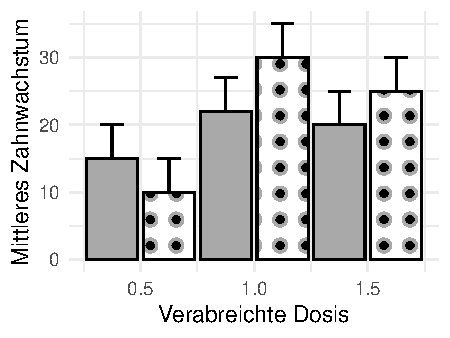
\includegraphics[width=\maxwidth]{img/mc-anova-02-a-1} 

}







\begin{enumerate}
\item [\textbf{A} \msquare] Eine negative Interaktion liegt vor $(\rho \geq 0.5)$.
\item [\textbf{B} \msquare] Eine mittlere bis starke Interaktion liegt vor $(p \leq 0.05)$
\item [\textbf{C} \msquare] Eine positive Interaktion liegt vor $(\rho \leq -0.5)$ 
\item [\textbf{D} \msquare] Eine Korrelation liegt vor $(p \leq 0.05)$.
\item [\textbf{E} \msquare] Keine Interaktion liegt vor $(p \leq 0.05)$.
\end{enumerate} 
\section*{Deskriptive Statistik \& Explorative Datenanalyse}

\section{Aufgabe \hfill (2 Punkte)}




Gegeben ist $y$ mit 12, 8, 12, 11 und 14. Berechnen Sie den Mittelwert und Standardabweichung.



\begin{enumerate}
\item [\textbf{A} \msquare] Es ergibt sich 10.4 +/- 2.4
\item [\textbf{B} \msquare] Es berechnet sich 11.4 +/- 4.8
\item [\textbf{C} \msquare] Es ergibt sich 12.4 +/- 1.095
\item [\textbf{D} \msquare] Sie erhalten 11.4 +/- 2.19
\item [\textbf{E} \msquare] Es berechnet sich 12.4 +/- 4.8
\end{enumerate} 

\section{Aufgabe \hfill (2 Punkte)}




Berechnen Sie den Median, das $1^{st}$ Quartile sowie das $3^{rd}$ Quartile von $y$ mit 22, 15, 6, 12, 32, 21 und 42.




\begin{enumerate}
\item [\textbf{A} \msquare] Es ergibt sich 21 +/- 12
\item [\textbf{B} \msquare] Es ergibt sich 21 +/- 12
\item [\textbf{C} \msquare] Es berechnet sich 21 [13; 33]
\item [\textbf{D} \msquare] Es ergibt sich 21 [12; 32]
\item [\textbf{E} \msquare] Sie erhalten 21 +/- 32
\end{enumerate} 

\section{Aufgabe \hfill (2 Punkte)}



Die empfohlene Mindestanzahl an Beobachtungen für die Visualisierung mit einem Histogramm sind...



\begin{enumerate}
\item [\textbf{A} \msquare] Wir sollten zwei bis fünf Beobachtungen mindestens pro Gruppe vorliegen haben.
\item [\textbf{B} \msquare] Wir brauchen fünf oder mehr Beobachtungen.
\item [\textbf{C} \msquare] 10 Beobachtungen.
\item [\textbf{D} \msquare] Die untere Grenze liegt bei einer Beobachtung.
\item [\textbf{E} \msquare] 1 Beobachtung.
\end{enumerate}

\section{Aufgabe \hfill (2 Punkte)}



Die Standardabweichung ist eine bedeutende deskriptive Statistik für die Analyse von Daten. Wie müssen Sie vorgehen um die Standardabweichung zu berechnen?



\begin{enumerate}
\item [\textbf{A} \msquare] Den Mittelwert berechen, dann die absoluten Abstände zum Mittelwert aufsummieren
\item [\textbf{B} \msquare] Den Median berechen, dann die quadratischen Abstände zum Median aufsummieren, dann die Wurzel ziehen.
\item [\textbf{C} \msquare] Den Mittelwert berechnen und die Abstände quadrieren. Die Summe mit der Fallzahl multiplizieren.
\item [\textbf{D} \msquare] Als erstes berechnen wir den Mittelwert. Dann bilden wir die Summe der quadratischen Abstände zu dem Mittelwert. Abschließend teilen wir durch die Fallzahl.
\item [\textbf{E} \msquare] Wir berechnen erst den Mittelwert und dann die quadratischen Abstände zu dem Mittelwert. Diese quadratischen Abstände summieren wir auf und teilen am Ende durch die Fallzahl. Als letzten Schritt ziehen wir die quadratische Wurzel.
\end{enumerate} 

\section{Aufgabe \hfill (2 Punkte)}



In Ihrer Abschlußarbeit wolllen Sie Ihre Daten für den Ertrag in einem Barplot darstellen. Sie nutzen den Barplot auch, da der Barplot zu den meist genutzten Visualiserungen von Daten gehört. Welche statistischen Maßzahlen stellt der Barplot dar?

 



\begin{enumerate}
\item [\textbf{A} \msquare] Der Barplot stellt die Mittelwerte und die Varianz dar.
\item [\textbf{B} \msquare] Durch die Abbildung des Barplot erhalten wir die Informationen über die Mittelwerte und die Varianz.
\item [\textbf{C} \msquare] Den Mittelwert und die Varianz.
\item [\textbf{D} \msquare] Durch die Abbildung des Barplot erhalten wir die Informationen über die Mittelwerte und die Standardabweichung.
\item [\textbf{E} \msquare] Den Median und die Quartile.
\end{enumerate}

\section{Aufgabe \hfill (2 Punkte)}



In Ihrer Abschlussarbeit zuErdbeeren finden Sie aufeinmal seltsame Daten. Jedenfalls kommt Ihnen das so vor. Daher berechnen Sie den Mittelwert und den Median. Der Mittelwert $\bar{y}$ und der Median $\tilde{y}$ unterscheiden sich. Welche Aussage ist richtig?



\begin{enumerate}
\item [\textbf{A} \msquare] Der Mittelwert und der Median sollten gleich sein, wenn Outlier in den Daten vorliegen. 
\item [\textbf{B} \msquare] Da sich der Mittelwert und der Median nicht unterscheiden, liegen vermutlich keine Outlier in den Daten vor. Wir verweden den Datensatz so wie er ist.
\item [\textbf{C} \msquare] Wenn sich der Mittelwert und der Median nicht unterscheiden, liegen vermutlich Outlier in den Daten vor.
\item [\textbf{D} \msquare] Der Mittelwert und der Median sollten gleich sein, wenn keine Outlier in den Daten vorliegen. 
\item [\textbf{E} \msquare] Wenn sich der Mittelwert und der Median unterscheiden, liegen vermutlich keine Outlier in den Daten vor.
\end{enumerate}

\section{Aufgabe \hfill (2 Punkte)}



Ihre Betreuung der Abschlussarbeit fragt überraschend in der letzten Besprechung, ob Ihre Messwerte einer Varianzhomogenität genügen. Sonst könnten Sie ja gar nicht einen t-Test rechnen. Da Ihnen die Zeit wegrennt, entscheiden Sie sich für eine schnelle Visualisierung im Anhang. Welche Visualisierung nutzen Sie und welche Regel kommt zur Abschätzung einer Varianzhomogenität zur Anwendung?



\begin{enumerate}
\item [\textbf{A} \msquare] Einen Barplot. Die Mittelwerte müssen alle auf einer Höhe liegen. Die Fehlerbalken haben hier keine Informationen.
\item [\textbf{B} \msquare] Einen Violinplot. Der Bauch der Violine muss hierbei einen höhren Wert annehmen als der Steg der Violine. Dann kann die Annahme einer Varianzhomogenität angenommen werden.
\item [\textbf{C} \msquare] In einer explorativen Datanalyse nutzen wir den Boxplot. Dabei sollte der Median als dicke Linie in der Mitte der Box liegen. Dann können wir von einer Varianzhomogenität ausgehen.
\item [\textbf{D} \msquare] Wir erstellen uns für jede Behandlung einen Dotplot und schauen, ob die Dots und damit die Varianz für jede Behandlung gleich groß sind.
\item [\textbf{E} \msquare] Einen Boxplot. Das IQR muss über alle Behandlungen zusammen mit den Whiskers ungefähr gleich aussehen.
\end{enumerate}

\section{Aufgabe \hfill (2 Punkte)}




In der Statistik müssen wir häufig überprüfen, ob unser Outcome einer bestimmten Verteilung folgt. Meistens überprüfen wir, ob eine
Normalverteilung vorliegt. Folgende drei Abbildungen eigenen sich im Besonderen für die Überprüfung einer Verteilungsannahme an eine Variable.





\begin{enumerate}
\item [\textbf{A} \msquare] Scatterplot, Densityplot, Barplot
\item [\textbf{B} \msquare] Boxplot, Violinplot, Mosaicplot
\item [\textbf{C} \msquare] Barplot, Mosaicplot, Violinplot
\item [\textbf{D} \msquare] Scatterplot, Mosaicplot, Boxplot
\item [\textbf{E} \msquare] Boxplot, Densityplot, Violinplot
\end{enumerate} 

\section{Aufgabe \hfill (2 Punkte)}



In dem folgenden Histogramm von $n = 205$ Pflanzen ist welche Verteilung abgebildet?



{\centering 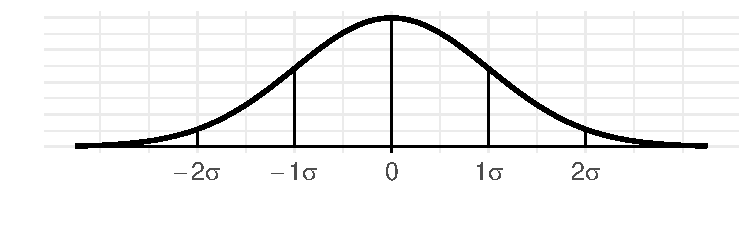
\includegraphics[width=\maxwidth]{img/mc-distribution-02-a-1} 

}







\begin{enumerate}
\item [\textbf{A} \msquare] Dem Histogramm entnehmen wir eine Possion-Verteilung.
\item [\textbf{B} \msquare] In dem Histogramm ist eine Ordinalverteilung dargestellt.
\item [\textbf{C} \msquare] Wir haben eine Normalverteilung vorliegen.
\item [\textbf{D} \msquare] Wir haben eine Gammaverteilung vorliegen.
\item [\textbf{E} \msquare] Eine Standardnormalverteilung.
\end{enumerate} 
\section*{Lineare Regression \& Korrelation}

\section{Aufgabe \hfill (2 Punkte)}



Sie haben das Modell $Y \sim X$ vorliegen und wollen nun ein kausales Modell rechnen. Welche Aussage ist richtig?



\begin{enumerate}
\item [\textbf{A} \msquare] Wir modellieren den Zusammenhang zwischen $X$ und $Y$ wenn ein kausales Modell rerechnet wird. Dabei kann nicht der gesamte Datensatz genutzt werden. Es wird ein Trainingsdatensatz zum Trainieren des Modells benötigt.
\item [\textbf{B} \msquare] Wir modellieren den Zusammenhang zwischen $X$ und $Y$ wenn ein kausales Modell rerechnet wird. Dabei kann der gesamte Datensatz genutzt werden. Eine Aufteilung wie in einem prädiktiven Modell ist nicht notwendig.
\item [\textbf{C} \msquare] Ein kausales Modell wird auf einem Trainingsdatensatz trainiert und anschliessend über eine explorative Datenanalyse validiert. Signifikanzen über $\beta_i$ können hier nicht festgestellt werden.
\item [\textbf{D} \msquare] Ein kausales Modell basiert auf einem Traingsdatensatz und einem Testdatensatz. Auf dem Trainingsdatensatz wird das Modell trainiert und auf dem Testdatensatz validiert.
\item [\textbf{E} \msquare] Ein kausales Modell benötigt mindestens eine Fallzahl von über 100 Beobachtungen und darf keine fehlenden Werte beinhalten. Die Varianzkomponenten müssen homogen sein.
\end{enumerate}

\section{Aufgabe \hfill (2 Punkte)}



Nach der Modellierung einer Regression stellt sich die Frage, ob die Residuen approximativ einer Normalverteilung folgen. Sie können einen QQ-Plot für die visuelle Überprüfung der Annahme an die Residuen nutzen. Welche Aussage ist richtig?



{\centering 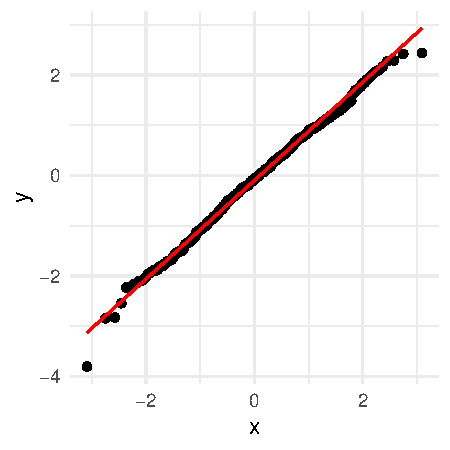
\includegraphics[width=\maxwidth]{img/mc-regression-05-a-1} 

}







\begin{enumerate}
\item [\textbf{A} \msquare] Wir betrachten die Punkte. Wenn die Punkte einigermaßen gleichmäßig verteilt liegen, dann gehen wir von normalen Residuen aus.
\item [\textbf{B} \msquare] Die Annahme der normalverteilten Residuen ist erfüllt. Die Punkte liegen zum überwiegenden Teil nicht auf der Geraden.
\item [\textbf{C} \msquare] Wir betrachten die Gerade, die durch die einzelnen Punkte laufen sollte. Wenn die 95\% der Punkte von der Geraden getroffen werden, dann gehen wir von normalverteilten Residuen aus.
\item [\textbf{D} \msquare] Wir betrachten die Gerade und dabei insbesondere die beiden Enden der Gerade in dem IQR, also dem ersten und dritten Quartile. Hier sollten die Punkte auf der Geraden liegen, dann ist die Annahme an die Normalverteilung der Residuen erfüllt.
\item [\textbf{E} \msquare] Die Annahme der normalverteilten Residuen ist erfüllt. Die Punkte liegen zum überwiegenden Teil auf der Geraden.
\end{enumerate}

\section{Aufgabe \hfill (2 Punkte)}



Nach einer Regressions sollten die Residuen (\texttt{.resid}) gleichmäßig um die Gerade verortet sein. Was bei einer simplen Regression noch relativ einfach visuell in einem Scatterplot zu überprüfen ist. Für komplexere Modell liefert der Residual Plot die notwendigen Informationen. Welche Aussage ist richtig?



{\centering 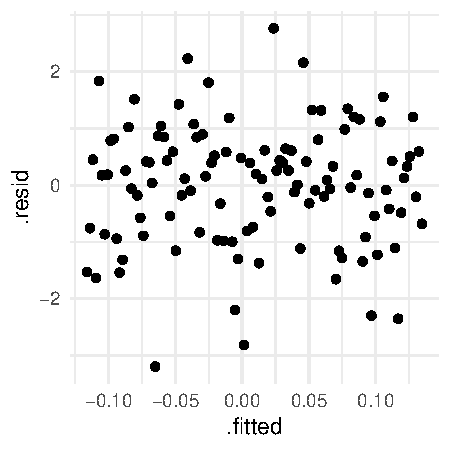
\includegraphics[width=\maxwidth]{img/mc-regression-06-a-1} 

}







\begin{enumerate}
\item [\textbf{A} \msquare] Die Annahme der normalverteilten Residuen ist nicht erfüllt. Vereinzelte Punkte liegen oberhalb bzw. unterhalb der Geraden um die 0 Linie weiter entfernt. Ein klares Muster ist zu erkennen.
\item [\textbf{B} \msquare] Wenn wir die Nulllinie betrachten so liegen die Punkte nicht gleichmäßig über und unter der Nulllinie. Unser Modell erfüllt nicht die Annahme von normalverteilten Residuen mit einem Mittelwert von 0 und einer Streuung von $s^2$.
\item [\textbf{C} \msquare] Die Annahme der normalverteilten Residuen ist erfüllt. Es ist ein Muster zu erkennen und wir können damit auf die Signifkanz von $x_1, ..., x_p$ schließen.
\item [\textbf{D} \msquare] Die Punkte müssen gleichmäßig in dem negativen Bereich liegen. Dies ist hier klar nicht der Fall. Einzelne Ausreißer können beobachtet werden. Die Analyse ist gescheitert.
\item [\textbf{E} \msquare] Die Annahme der normalverteilten Residuen ist erfüllt. Kein Muster ist zu erkennen und keine Outlier zu beobachten.
\end{enumerate}

\section{Aufgabe \hfill (2 Punkte)}




Sie berechnen in Ihgrer Abschlussarbeit den Korrelationskoeffizienten $\rho$. Welche Aussage über den Korrelationskoeffizienten $\rho$ ist richtig?




\begin{enumerate}
\item [\textbf{A} \msquare] Der Korrelationskoeffizienten $\rho$ liegt zwischen -1 und 1. Darüber hinaus ist der Korrelationskoeffizienten $\rho$ als standardisierte Steigung zu verstehen, wenn eine Standardisierung durchgeführt wurde. Diese Adjustierung nach Fischer muss am Anschluß der Berechnung der Korrelation durchgeführt werden.
\item [\textbf{B} \msquare] Korrelationskoeffizienten $\rho$ liegt zwischen 0 und 1. Darüber hinaus ist der Korrelationskoeffizienten $\rho$ einheitslos und kann als Standardisierung verstanden werden.
\item [\textbf{C} \msquare] Der Korrelationskoeffizienten $\rho$ ist eine veraltete Darstellungsform von Effekten in der linearen Regression und wird wie das $\eta^2$ aus der ANOVA interpretiert. Der Korrelationskoeffizienten $\rho$ beschreibt den Anteil an erklärter Varianz durch die Regression.
\item [\textbf{D} \msquare] Der Korrelationskoeffizienten $\rho$ zeigt keinen Zusammenhang zwischen zwei Variablen $x$ und $y$ bei einem Wert von 0. Einen maximalen negativen Zusammenhang bei -1 und somit auch einen maximalen positiven Zusammenhang bei 1. Korrelationskoeffizienten $\rho$ ist einheitslos.
\item [\textbf{E} \msquare] Der Korrelationskoeffizienten $\rho$ zeigt keinen Zusammenhang zwischen zwei Variablen $x$ und $y$ bei einem Wert von 0. Einen negativen Zusammenhang Richtung -1 und somit auch einen positiven Zusammenhang Richtung 1. Je größer die Zahl allgemein, desto stärker der Effekt.
\end{enumerate}

\section{Aufgabe \hfill (2 Punkte)}



In einer lineren Regression kann es vorkommen, dass der Effekt repräsentiert durch den $\beta$ Koeffizienten nicht so richtig von der Größenordnung zu dem p-Wert passen will. So liefert eine Untersuchung des Einflusses von der $Fe_3O_4$-Konzentration in [$\mu g$] im Wasser auf das Trockengewicht in [$kg$] an Wasserlinsen folgende Effekte und p-Werte: $2e-04$ als p-Wert und einen $\beta_{Fe_3O_4}$ Koeffizienten von $7.4\times 10^{-6}$. Welche Aussage ist richtig?




\begin{enumerate}
\item [\textbf{A} \msquare] Die Einheit der $Fe_3O_4$-Konzentration ist zu klein gewählt. Die Erhöhung der $Fe_3O_4$-Konzentration um 1 Einheit führt nur zu einem sehr winzigen Anstieg von $\beta_{Fe_3O_4}$ im Gewicht der Wasserlinsen. Die Einheit [$\mu g$] muss besser gewählt werden.
\item [\textbf{B} \msquare] Die Fallzahl ist zu hoch angesetzt. Je höher die Fallzahl ist, desto kleiner ist die Teststatistik und damit ist dann auch der $p$-Wert sehr klein. Es sollte über eine Reduzierung der Fallzahl nachgedacht werden. Dann sollte der Effekt zum p-Wert passen.
\item [\textbf{C} \msquare] Die Einheit der $Fe_3O_4$-Konzentration ist zu klein gewählt. Dadurch sehen wir den sehr kleinen $p$-Wert. Der $p$-Wert und die Einheit von der $Fe_3O_4$-Konzentration hängen antiproportional zusammen.
\item [\textbf{D} \msquare] Wenn der Effekt $\beta_{Fe_3O_4}$ winzig ist, dann kann es an einer falsch gewählten Einheit liegen. Der Anstieg von einer Einheit in $X$ führt ja zu einer Änderung von $\beta_{Fe_3O_4}$ in $x$. Wir müssen daher die Einheit von $y$ entsprechend anpassen.
\item [\textbf{E} \msquare] Die Fallzahl ist zu klein angesetzt. Je kleiner die Fallzahl ist, desto höher ist die Teststatsitik und damit auch der $p$-Wert kleiner. Wir brauchen also mehr Fallzahl um den geringen Effekt noch signifikant zu krigen.
\end{enumerate}

\section{Aufgabe \hfill (2 Punkte)}



Neben der klassischen Regression kann die Funktion \texttt{lm()} in \Rlogo auch für welche andere Art von Anwendung genutzt werden?





\begin{enumerate}
\item [\textbf{A} \msquare] Die Funktion \texttt{lm()} berechnet die Varianzstruktur für eine ANOVA. Dannach kann dann über eine explorative Datenalayse nochmal eine Signifikanz berechnet werden. Sollte vor der Verwendung der Funktion \texttt{lm()} schon eine EDA gerechnet worden sein, so ist die Analyse wertlos.
\item [\textbf{B} \msquare] Ist die Einflussvariable $X$ ein Faktor so werden die Gruppenmittelwerte geschätzt und eine anschließende ANOVA sowie multipler Gruppenvergleich mit \{emmeans\} ist möglich. Dennoch muss zuerst ein lineares Modell mit der Funktion \texttt{lm()} in \Rlogo gerechnet werden.
\item [\textbf{C} \msquare] Ist die Einflussvariable $X$ numerisch so werden die Gruppenmittelwerte geschätzt und eine anschließende ANOVA sowie multipler Gruppenvergleich mit \{emmeans\} ist möglich.
\item [\textbf{D} \msquare] Die Funktion \texttt{lm()} in \Rlogo wird klassischerweise für die nicht-lineare Regression genutzt. Ist die Einflussvariable $X$ numerisch so werden die Gruppenmittelwerte geschätzt.
\item [\textbf{E} \msquare] Ist die Einflussvariable $X$ ein Faktor so werden die Gruppenmittelwerte geschätzt und eine anschließende ANOVA sowie multipler Gruppenvergleich mit \{emmeans\} ist möglich. Die Funktion \texttt{lm()} kann dabei eigentlich weggelassen werden, wird aber traditionell gerechnet.
\end{enumerate}

\section{Aufgabe \hfill (2 Punkte)}



Welche Aussage über das \textit{generalisierte lineare Modell (GLM)} ist richtig?




\begin{enumerate}
\item [\textbf{A} \msquare] Das \textit{generalisierte lineare Modell (GLM)} erlaubt auch weitere Verteilungsgruppen für das $X$ bzw. die Einflussvariablen in einer linearen Regression zu wählen.
\item [\textbf{B} \msquare] Das GLM ist eine allgemeine Erweiterung der linearen Regression auf die Normalverteilung.
\item [\textbf{C} \msquare] Dank dem \textit{generalisierten linearen Modell (GLM)} können auch andere Verteilungsfamilien als die Normalverteilung mit einer linearen Regression modelliert werden.
\item [\textbf{D} \msquare] Dank dem \textit{generalisierten linearen Modell (GLM)} können auch andere Verteilungsfamilien -- außer die Normalverteilung -- mit einer linearen Regression modelliert werden. Dafür werden alle Verteilungen in eine Normalverteilung überführt und anschließend standardisiert.
\item [\textbf{E} \msquare] Das GLM ist ein faktisch maschineller Lernalgorithmus, der selstständig die Verteilungsfamilie für Y wählt.
\end{enumerate}
\section*{Vermischte Themen}  

\section{Aufgabe \hfill (2 Punkte)}

Die Randomisierung von Beobachtungen zu den Versuchseinheiten
ist bedeutend in der Versuchsplanung. Welche der folgenden Aussagen ist richtig?



\begin{enumerate}
\item [\textbf{A} \msquare] Durch eine Randomisierung können wir nicht von Strukturgleichheit zwischen der Stichprobe und der Grundgesamtheit ausgehen.
\item [\textbf{B} \msquare] Randomisierung bringt starke Unstrukturiertheit in das Experiment und erlaubt erst von der Stichprobe auf die Grundgesamtheit zurückzuschliessen.
\item [\textbf{C} \msquare] Strukturgleichheit ist durch Randomisierung gegeben. Somit kann von der Stichprobe auf die Grundgesamtheit geschlossen werden
\item [\textbf{D} \msquare] Randomisierung ist die direkte Folge von Strukturgleichheit. Die Strukturgleichheit erlaubt es erst von der Stichprobe auf die Grundgesamtheit zurückzuschliessen.
\item [\textbf{E} \msquare] Strukturgleichheit ist durch Randomisierung gegeben. Leider hilft die Randomisierung noch nicht um von der Stichprobe auf die Grundgesamtheit zu schließen. Deshalb wurde das Falsifikationsprinzip entwickelt.
\end{enumerate}

\section{Aufgabe \hfill (2 Punkte)}



Viele wissenschaftliche Orginalquellen sind in Englisch verfasst. Jetzt finden Sie heraus, dass auch \Rlogo nur in englischer Sprache funktioniert. Warum ist das so?



\begin{enumerate}
\item [\textbf{A} \msquare] \Rlogo Pakete sind nur in englischer Sprache verfasst. Es macht keinen Sinn \Rlogo daher in Deutsch zu bedienen.
\item [\textbf{B} \msquare] Alle Funktionen und auch Anwendungen sind in \Rlogo in englischer Sprache. Die Nutzung von deutschen Wörtern ist nicht schick und das ist zu vermeiden.
\item [\textbf{C} \msquare] Die Spracherkennung von \Rlogo ist nicht in der Lage Deutsch zu verstehen.
\item [\textbf{D} \msquare] Programmiersprachen können nur englische Begriffe verarbeiten. Zusätzliche Pakete können zwar geladen werden, aber meist funktionieren diese Pakete nicht richtig. Deutsch ist International nicht bedeutend genug.
\item [\textbf{E} \msquare] Die \Rlogo Pakete sind nur in englischer Sprache verfasst. Das ist aber nicht der Hauptgrund, denn \Rlogo hat wie alle Programmiersprachen Probelem mit Umlauten und Sonderzeichen.
\end{enumerate}

\section{Aufgabe \hfill (2 Punkte)}



Bei der explorativen Datenanalyse (EDA) in \Rlogo gibt es eine richtige Abfolge von Prozessschritten, auch 	extit{Circle of life} genannt. Wie lautet die richtige Reihenfolge für die Erstellung einer EDA?



\begin{enumerate}
\item [\textbf{A} \msquare] Wir lesen die Daten ein und mutieren die Daten. Dabei ist wichtig, dass wir nicht das Paket \texttt{tidyverse} nutzen, da dieses Paket veraltet ist. über die Funktion \texttt{library(tidyverse)} entfernen wir das Paket von der Analyse.
\item [\textbf{B} \msquare] Wir lesen die Daten über eine generische Funktion \texttt{read()} ein und müssen dann die Funktion \texttt{ggplot()} nur noch installieren. Dann haben wir die Abbildungen als \texttt{*.png} vorliegen.
\item [\textbf{C} \msquare] Wir lesen als erstes die Daten über \texttt{read\_excel()} ein, transformieren die Spalten über \texttt{mutate()} in die richtige Form und können dann  über \text{ggplot()} uns die Abbildungen erstellen lassen. Wichtig ist, dass wir keine Faktoren sondern nur numerische Variablen vorliegen haben.
\item [\textbf{D} \msquare] Für eine explorativen Datenanalyse (EDA) in \Rlogo müssen wir als erstes die Daten über \texttt{read\_excel()} einlesen. Danach müssen wir schauen, dass wir die Zeilen richtig über \texttt{mutate()} transformiert haben. Insbesondere müssen Variablen mit kontinuierlichen Werten in einen Faktor umgewandelt werden. Am Ende nutzen wir die Funktion \text{ggplot()} für die eigentlich EDA.
\item [\textbf{E} \msquare] Für eine explorativen Datenanalyse (EDA) in \Rlogo müssen wir als erstes die Daten über \texttt{read\_excel()} einlesen. Danach müssen wir schauen, dass wir die Spalten richtig über \texttt{mutate()} transformiert haben. Insbesondere müssen Variablen mit Kategorien in einen Faktor umgewandelt werden. Am Ende nutzen wir die Funktion \text{ggplot()} für die eigentlich EDA.
\end{enumerate}

\section{Aufgabe \hfill (2 Punkte)}



Es sei $s^2_1 = s^2_2$ in dem Modell $Y \sim X$. Welche Aussage ist richtig?



\begin{enumerate}
\item [\textbf{A} \msquare] Es handelt sich um ein unbalanciertes Design.
\item [\textbf{B} \msquare] Es liegt Varianzhetrogenität vor.
\item [\textbf{C} \msquare] Es handelt sich um ein balanciertes Design.
\item [\textbf{D} \msquare] Es handelt sich um unabhängige Beobachtungen.
\item [\textbf{E} \msquare] Es liegt Varianzhomogenität vor.
\end{enumerate}

\section{Aufgabe \hfill (2 Punkte)}



In einem Zuchtexperiment messen wir die Ferkel verschiedener Sauen. Die Ferkel einer Muttersau sind daher im statistischen Sinne...



\begin{enumerate}
\item [\textbf{A} \msquare] Untereinander unabhängig. Die Ferkel sind eigenständig und benötigen keine zusätzliche Behandlung.
\item [\textbf{B} \msquare] Untereinander stark korreliert. Die Ferkel sind von einer Mutter und sommit miteinander korreliert. Dies wird in der Statistik jedoch meist nicht modelliert.
\item [\textbf{C} \msquare] Die Ferkel stammen von der gleichen Sau und sind somit untereinander abhängig.
\item [\textbf{D} \msquare] Untereinander unabhängig. Sollten die Mütter verwandt sein, so ist die Varianzstruktur ähnlich und muss modelliert werden.
\item [\textbf{E} \msquare] Die Ferkel stammen von der gleichen Sau und sind somit untereinander unabhängig.
\end{enumerate}

\section{Aufgabe \hfill (2 Punkte)}



Neben der Mittelwertsdifferenz als Effektschätzer bei normalverteilten Endpunkten wird auch häufig der Effektschätzer Risk ratio bei binären Endpunkten verwendet. Welche Aussage über den Effektschätzer Risk ratio ist im folgenden Beispiel zur Behandlung von Klaueninfektionen bei Schweinen richtig? Dabei sind 6 Tiere krank und 8 Tiere sind gesund.



\begin{enumerate}
\item [\textbf{A} \msquare] Das Verhältnis der Chancen Risk ratio ergibt ein Chancenverhältnis von 0.43. Wir sind an der Chance krank zu sein interessiert.
\item [\textbf{B} \msquare] Da es sich um ein Chancenverhältnis handelt ergibt sich ein Risk ratio von 2.33.
\item [\textbf{C} \msquare] Das Verhältnis der Anteile Risk ratio ergibt ein Anteilsverhältnis von 0.43. Wir sind am Anteil der Kranken interessiert.
\item [\textbf{D} \msquare] Da es sich um ein Chancenverhältnis handelt ergibt sich ein Risk ratio von 0.75.
\item [\textbf{E} \msquare] Es ergibt sich ein Risk ratio von 0.43, da es sich um eine Chancenverhältnis handelt.
\end{enumerate}

\section{Aufgabe \hfill (2 Punkte)}



Sie werten in Ihrer Abschlussarbeit einen sehr großen Datensatz aus einer öffentlichen Datenbank aus. Nun stellen Sie fest, dass Sie ein Problem mit der Bewertung Ihrer Ergbnisse anhand der Signifikanz bekommen. Wie Sie herausfinden, scheint dies ein häufiges Problem in der Bio Data Science zu sein. Welche Aussage ist richtig?




\begin{enumerate}
\item [\textbf{A} \msquare] Aktuell werden immer größere Datensätze erhoben. Eine erhöhte Fallzahl führt automatisch auch zu mehr signifikanten Ergebnissen, selbst wenn die eigentlichen Effekte nicht relevant sind.
\item [\textbf{B} \msquare] Mehr Fallzahl in Datensätzen bedeutet mehr signifikante Ergebnisse, da in mehr Daten auch mehr Informationen beinhaltet sind. Deshalb lohnen sich riesige Datensätze, die durch die vielen signifikanten Ergebnisse auch eine Menge an relevanten Erkenntnissen liefern.
\item [\textbf{C} \msquare] Relevanz und Signifikanz haben nichts miteinander zu tun. Daher gibt es auch keinen Zusammenhang zwischen hoher Fahlzahl (n > 10000) und einem signifikanten Test. Ein Effekt ist immer relevant und somit signifikant.
\item [\textbf{D} \msquare] Big Data ist ein Problem der parametrischen Statistik. Parameter lassen sich nur auf kleinen Datensätzen berechnen, da es sich sonst nicht mehr um eine Stichprobe im engen Sinne der Statistik handelt.
\item [\textbf{E} \msquare] Aktuell werden immer größere Datensätze erhoben. Dadurch wird auch die Varianz immer höher was automatisch zu mehr signifikanten Ergebnissen führt.
\end{enumerate}
\section*{Multiple Gruppenvergleiche}    

\section{Aufgabe \hfill (2 Punkte)}



Sie haben folgende unadjustierten p-Werte gegeben: 0.001, 0.03, 0.34, 0.02 und 0.42. Sie adjustieren die p-Werte nach
Bonferroni. Welche Aussage ist richtig?



\begin{enumerate}
\item [\textbf{A} \msquare] Nach der Bonferroni-Adjustierung ergeben sich die adjustierten p-Werte von 0.005, 0.15, 1, 0.1 und 1. Die adjustierten p-Werte werden zu einem $\alpha$-Niveau von 1\% verglichen.
\item [\textbf{B} \msquare] Nach der Bonferroni-Adjustierung ergeben sich die adjustierten p-Werte von 0.005, 0.15, 1.7, 0.1 und 2.1. Die adjustierten p-Werte werden zu einem $\alpha$-Niveau von 5\% verglichen.
\item [\textbf{C} \msquare] Nach der Bonferroni-Adjustierung ergeben sich die adjustierten p-Werte von 2e-04, 0.006, 0.068, 0.004 und 0.084. Die adjustierten p-Werte werden zu einem $\alpha$-Niveau von 5\% verglichen.
\item [\textbf{D} \msquare] Nach der Bonferroni-Adjustierung ergeben sich die adjustierten p-Werte von 2e-04, 0.006, 0.068, 0.004 und 0.084. Die adjustierten p-Werte werden zu einem $\alpha$-Niveau von 1\% verglichen.
\item [\textbf{E} \msquare] Nach der Bonferroni-Adjustierung ergeben sich die adjustierten p-Werte von 0.005, 0.15, 1, 0.1 und 1. Die adjustierten p-Werte werden zu einem $\alpha$-Niveau von 5\% verglichen.
\end{enumerate}

\section{Aufgabe \hfill (2 Punkte)}



Die Abkürzung \textit{CLD} steht für welches statistische Verfahren? Welche folgende Beschreibung der Interpretation ist korrekt?



\begin{enumerate}
\item [\textbf{A} \msquare] Compact letter display. Teilweise ist die Interpretation des CLD schwierig, da wir ja nach Unterschieden suchen aber nur Gleichheit in den Buchstaben sehen. Die Gleichheit der Behandlungen wird durch gleiche Buchstaben dargestellt.
\item [\textbf{B} \msquare] Compound letter display. Gleichheit in dem Outcomes wird durch den gleichen Buchstaben oder Symbol dargestellt. Teilweise ist die Interpretation des Verbunds (eng. compound) herausfordernd, da wir ja nach dem Unterschied suchen.
\item [\textbf{C} \msquare] Compact letter detection. Gleichheit in den Behandlungen wird durch den gleichen Buchstaben oder Symbol dargestellt.
\item [\textbf{D} \msquare] Compact line display. Gleichheit in den Behandlungen wird durch den gleichen Buchstaben oder Symbol dargestellt. Früher wurden keine Buchstaben sondern eine durchgezogene Linie verwendet. Bei mehr als drei Gruppen funktioniert die Linie aber graphisch nicht mehr.
\item [\textbf{E} \msquare] Compact letter display. Gleiche Buchstaben bedeuten, dass sich die Behandlungen unterscheiden. Daher ist das CLD sehr unintuitiv. Es wäre besser, wenn gleiche Buchstaben Gleichheit anzeigen würden. Dies ist aber leider in der statistischen Testtheorie nicht möglich.
\end{enumerate}

\section{Aufgabe \hfill (2 Punkte)}




In Ihrer Bachelorarbeit müssen Sie einen Feldversuch auswerten. Nachdem Sie die zweifaktorielle ANOVA gerechnet haben und keine signifikante Interaktion vorliegt, wollen Sie jetzt einen Posthoc-Test rechnen. Welches R Paket nutzen Sie dafür am besten?



\begin{enumerate}
\item [\textbf{A} \msquare] Das R Paket \{emmeans\} erlaubt die Durchführung eines multiplen Gruppenvergleichs. Aus einem \{emmeans\} Objekt lässt sich recht einfach das CLD erstellen und so über Barplots eine schnelle Interpration der statistischen Auswertung durchführen.
\item [\textbf{B} \msquare] Das R Paket \{lm\}. Das Paket \{lm\} erstellt selbstständig Konfidenzintervalle und entsprechende p-Werte. Da wir in dem Paket nicht adjustieren müssen, ist es bei Anwendern sehr beliebt.
\item [\textbf{C} \msquare] Das R Paket \{hmisc\} erlaubt die Durchführung eines multiplen Gruppenvergleichs aus verschiedenen Modellen heraus. Aus einem hmisc Objekt lässt sich recht einfach das CLD erstellen und so über Barplots eine schnelle Interpration der statistischen Auswertung durchführen.
\item [\textbf{D} \msquare] Das R Paket \{ggplot\}. Wir erhalten hier sofort eine Visualisierung der Daten. Anhand der Visualisierung lässt sich eine explorative Datenanalyse durchführen, die gleichwertig zu einem Posthoc-Test ist.
\item [\textbf{E} \msquare] Das R Paket \{emmeans\} erlaubt die Durchführung eines multiplen Gruppenvergleichs. Aus einem emmeans Objekt lässt sich leider kein CLD erstellen. Dennoch ist das Paket einfach zu bedienen und wird deshalb genutzt. Die Interpretation der statistischen Auswertung wird über einen Barplot abgebildet.
\end{enumerate}

\section{Aufgabe \hfill (2 Punkte)}



Bei einem Posthoc-Test kann es zu einer überraschenden Besonderheit beim statistischen Testen kommen. Wie lautet der Fachbegriff und wie kann mit der überraschenden Besonderheit umgegangen werden?



\begin{enumerate}
\item [\textbf{A} \msquare] Das globale Signifikanzniveau liegt nicht mehr bei $5\%$ sondern sehr viel höher. Es kommt zu einer $\alpha$-Inflation. Dagegen kann mit der Adjustierung der p-Werte nach Bonferroni vorgegangen werden.
\item [\textbf{B} \msquare] Das globale Signifikanzniveau explodiert und erreicht Werte größer als Eins. Es kommt zu einer $\alpha$-Inflation. Dagegen kann mit der Adjustierung der $\alpha$-Werte nach Bonferroni vorgegangen werden.
\item [\textbf{C} \msquare] Die Adjustierung der p-Werte nach Bonferroni erlaubt es gegen die $\beta$-Inflation vorzugehen, die häufig beim multiplen Testen auftritt. Das globale Powerniveau liegt nicht mehr bei $80\%$ sondern sehr viel niedriger.
\item [\textbf{D} \msquare] Beim multiplen Testen kann es zu Varianzheterogenität kommen. Das globale Signifikanzniveau liegt nicht mehr bei $5\%$. Daher müssen die p-Werte entsprechend adjustiert werden. Das Verfahren nach Welch, bekannt aus dem t-Test, ist hier häufig anzuwenden.
\item [\textbf{E} \msquare] Das globale Signifikanzniveau liegt nicht mehr bei $5\%$ sondern sehr viel niedriger, bei ca. $1\%$. Es kommt zu einer $\alpha$-Hyperinflation. Dagegen kann mit der Adjustierung der p-Werte nach Bonferroni vorgegangen werden.
\end{enumerate}

\section{Aufgabe \hfill (2 Punkte)}




In Ihrer Bachelorarbeit werten Sie einen einfaktoriellen Versuch aus. Dafür rechnen Sie in \Rlogo zunächst eine ANOVA und schließen dann dann einen multiplen vergleich mit t-Tests an. Welche Aussage über die Effekte in Ihrem versuch ist richtig?



\begin{enumerate}
\item [\textbf{A} \msquare] Wenn ein multipler Test gerechnet wird, dann muss der Effekt $\Delta$ nicht adjustiert werden im Gegensatz zu den p-Werten.
\item [\textbf{B} \msquare] Beim multiplen Testen kann es zu einer Effektüberschätzung ($\Delta$-Inflation) kommen. Daher müssen die Effekte angepasst werden. Dies geschieht nicht händisch sondern intern in den angewendeten Algorithmen.
\item [\textbf{C} \msquare] Beim multiplen Testen werden die Effekte der paarweisen Vergleiche ignoriert. Der Nachteil des multiplen Testens ist ja auch, dass wir am Ende keine Effekte mehr vorliegen haben. Eine ANOVA liefert hier bessere Informationen.
\item [\textbf{D} \msquare] Wenn ein multipler Test gerechnet wird, dann muss der Effekt $\Delta$ nicht adjustiert werden. Bei einem Effekt im multiplen Testen handelt es sich um eine Wahrscheinlichkeit für das Auftreten der Nullhypothese.
\item [\textbf{E} \msquare] Beim multiplen Testen kann es zu einer $\Delta$-Inflation kommen. Das globale Effektniveau liegt nicht mehr bei $20\%$. Daher müssen die Effekte entsprechend adjustiert werden. Hierfür gibt es verschiedene Verfahren, wobei das Verfahren zur Adjustierung der Effekte nach Bonferroni das bekanneste Verfahren ist.
\end{enumerate}
\section*{Statistische Testtheorie}  

\section{Aufgabe \hfill (2 Punkte)}




Geben ist $Pr(D|H_0)$ als mathematischer Ausdruck, welche Aussage ist richtig?



\begin{enumerate}
\item [\textbf{A} \msquare] $Pr(D|H_0)$ beschreibt die Wahrscheinlichkeit die Teststatistik $T_D$ aus den Daten $D$ zu beobachten, wenn die Nullhypothese wahr ist.
\item [\textbf{B} \msquare] $Pr(D|H_0)$ ist die Wahrscheinlichkeit der Alternativehypothese und somit $1 - Pr(H_A)$
\item [\textbf{C} \msquare] Die Inverse der Wahrscheinlichkeit unter der die Nullhypothese nicht mehr die Alternativehypothese überdeckt.
\item [\textbf{D} \msquare] Die Wahrscheinlichkeit für die Nullhypothese, wenn die Daten wahr sind.
\item [\textbf{E} \msquare] $Pr(D|H_0)$ ist die Wahrscheinlichkeit nicht die Daten $D$ zu beobachten sondern die Nullhypothese, wenn diese wahr ist.
\end{enumerate}

\section{Aufgabe \hfill (2 Punkte)}



Die Testtheorie hat einen philosophischen Unterbau. Eins der Prinzipien ist das Falsifikationsprinzip. Das Falsifikationsprinzip besagt,



\begin{enumerate}
\item [\textbf{A} \msquare] ... dass Annahmen an statistische Modelle meist falsch sind.
\item [\textbf{B} \msquare] ... dass Fehlerterme in statistischen Modellen nicht verifiziert werden können.
\item [\textbf{C} \msquare] ... dass in der Wissenschaft immer etwas falsch sein muss. Sonst gebe es keinen Fortschritt.
\item [\textbf{D} \msquare] ... dass ein minderwertes Modell durch ein weniger minderwertiges Modell ersetzt wird. Es gilt das Falsifikationsprinzip nach Karl Popper.
\item [\textbf{E} \msquare] ... dass ein minderwertes Modell durch ein minderwertiges Modell ersetzt wird. Es gilt das Verifikationsprinzip nach Karl Popper.
\end{enumerate}

\section{Aufgabe \hfill (2 Punkte)}



In fast allen wissenschaftlichen Disziplinen liegt der Grenzwert für das Signifikanzniveau $\alpha$ bei 5\%. Wieso wurde dieser Konsens über die Signifikanzschwelle in dieser Form getroffen?



\begin{enumerate}
\item [\textbf{A} \msquare] Im Rahmen eines langen Disputs zwischen Neyman und Fischer wurde $\alpha = 5\%$ festgelegt. Leider werden die Randbedingungen und Voraussetzungen an statistsiche Modelle heute immer wieder ignoriert.
\item [\textbf{B} \msquare] Der Begründer der modernen Statistik, R. Fischer, hat die Grenze simuliert und berechnet. Dadurch ergibt sich dieser optimale Cut-Off.
\item [\textbf{C} \msquare] Da Wissenschaftler eine Schwelle für die statistische Testentscheidung benötigen wurde $\alpha$ in einer großen Konferenz 1945 gewählt. Damit ist $\alpha = 5\%$ eine Kulturkonstante mit einem Rank einer Naturkonstante.
\item [\textbf{D} \msquare] Als Kulturkonstante hat $\alpha = 5\%$ den Rang einer Naturkonstante und wurde nach langer Diskussion in der UN im Jahre 1983 festgesetzt. Damals auch schon mit der Zustimmung der UdSSR.
\item [\textbf{E} \msquare] Die Festlegung von $\alpha = 5\%$ ist eine Kulturkonstante. Wissenschaftler benötigt eine Schwelle für eine statistische Testentscheidung, der Wert von $\alpha$ wurde aber historisch mehr zufällig gewählt.
\end{enumerate}

\section{Aufgabe \hfill (2 Punkte)}

Betrachten wir die Teststatistik aus einem abstrakteren Blickwinkel. Beim
statistischen Testen wird das \textit{"`signal"'} mit dem
\textit{"`noise"'} aus den Daten $D$ zu einer Teststatistik $T_D$ verrechnet. Welche der Formel
berechnet korrekt die Teststatistik $T_D$?



\begin{enumerate}
\item [\textbf{A} \msquare] Es gilt $T_D = signal \cdot noise$
\item [\textbf{B} \msquare] Es gilt $T_D = \cfrac{noise}{signal}$
\item [\textbf{C} \msquare] Es gilt $T_D = \cfrac{signal}{noise^2}$
\item [\textbf{D} \msquare] Es gilt $T_D = (signal \cdot noise)^2$
\item [\textbf{E} \msquare] Es gilt $T_D = \cfrac{signal}{noise}$
\end{enumerate}

%% ------------------------------------------------------------

\section{Aufgabe \hfill (2 Punkte)}



In der Theorie zur statistischen Testentscheidung kann folgende Aussage
in welche richtige Analogie gesetzt werden?

\begin{center}
\textit{$H_0$ ablehnen obwohl die $H_0$ gilt}
\end{center}



\begin{enumerate}
\item [\textbf{A} \msquare] In die Analogie eines Rauchmelders: \textit{Alarm with fire}.
\item [\textbf{B} \msquare] In die Analogie eines brennenden Hauses ohne Rauchmelder: \textit{House without noise}.
\item [\textbf{C} \msquare] \textit{Alarm without fire}, dem $\alpha$-Fehler in der Analogie eines Rauchmelders.
\item [\textbf{D} \msquare] \textit{Alarm with fire}, dem $\alpha$-Fehler in der Analogie von Feuer.
\item [\textbf{E} \msquare] \textit{Fire without alarm}, dem $\beta$-Fehler als Analogie eines Rauchmelders.
\end{enumerate}

\section{Aufgabe \hfill (2 Punkte)}



Welche statistische Maßzahl erlaubt es Relevanz mit Signifikanz zu verbinden? Welche Aussage ist richtig?



\begin{enumerate}
\item [\textbf{A} \msquare] Das $\Delta$. Durch die Effektstärke haben wir einen Wert für die Relevanz, die vom Anwender bewertet werden muss. Da $\Delta$ antiproportional zum p-Wert ist, bedeutet auch ein hohes $\Delta$ ein sehr kleinen p-Wert.
\item [\textbf{B} \msquare] Über das Konfidenzintervall. Das Konfidenzinterval beitet eine Entscheidung über die Signifikanz und zusätzlich kann über die Visualizierung des Konfidenzintervals eine Relevanzschwelle definiert werden.
\item [\textbf{C} \msquare] Der p-Wert. Durch den Vergleich mit $\alpha$ lässt sich über die Signifikanz entscheiden und der $\beta$-Fehler erlaubt über die Power eine Einschätzung der Relevanz.
\item [\textbf{D} \msquare] Das OR. Als Chancenverhältnis gibt es das Verhältnis von Relevanz und Signifikanz wieder.
\item [\textbf{E} \msquare] Einem Konfidenzintervall. Das Konfidenzinterval bringt durch eine Visualisierung und drei Intervallgrenzen die Möglichkeit mit, eine Relevanzschwelle neben der Signifikanzschwelle und der $\alpha$-Schwelle zu definieren.
\end{enumerate}

\section{Aufgabe \hfill (2 Punkte)}



Welche Aussage über den $p$-Wert und dem Signifikanzniveau $\alpha$ gleich 5\% ist richtig?



\begin{enumerate}
\item [\textbf{A} \msquare] Wir machen ein Aussage über die Flächen und zwischen den Kurve der Teststatistiken der Hypothesen $H_0$ und $H_A$, wenn die $H_0$ gilt. Dabei werden Wahrscheinlichkeiten vergleichen, die durch die Flächen unter der Kurve repräsentiert werden.
\item [\textbf{B} \msquare] Wir machen ein Aussage über die Flächen und der Kurve der Teststatistik, wenn die $H_0$ gilt. Dabei werden Wahrscheinlichkeiten vergleichen, die durch die Flächen unter der Kurve repräsentiert werden.
\item [\textbf{C} \msquare] Wir vergleichen mit dem $p$-Wert und dem Signifikanzniveau $\alpha$ Wahrscheinlichkeiten und damit die absoluten Werte auf einem Zahlenstrahl, wenn die $H_0$ gilt.
\item [\textbf{D} \msquare] Wir vergleichen mit dem $p$-Wert und dem Signifikanzniveau $\alpha$ absolute Werte auf einem Zahlenstrahl und damit den Unterschied der Teststatistiken, wenn die $H_0$ gilt.
\item [\textbf{E} \msquare] Wir machen eine Aussage über die indivduelle Wahrscheinlichkeit des Eintretens der Nullhypothese $H_0$. Der $p$-Wert wird mit dem Signifikanzniveau verglichen und bewertet.
\end{enumerate}

\section{Aufgabe \hfill (2 Punkte)}



Um die Testtheorie besser zu verstehen, mag es manchmal sinnvoll sein ein Beispiel aus dem Alltag zu wählen. Die Ergebnisse der Analyse durch einen statistischen Test können auch in grobe Analogie zur Wettervorhersage gebracht werden. Welche Aussage trifft am ehesten zu?



\begin{enumerate}
\item [\textbf{A} \msquare] In der Analogie der Regenwahrscheinlichkeit: ein statistischer Test gibt die Wahrscheinlichkeit für das Auftreten eines Ereignisses wieder. Die Stärke des Effektes wird nicht wiedergeben.
\item [\textbf{B} \msquare] In der Analogie der Sonnenscheindauer: Wie lange kann mit einem entsprechenden Effekt gerechnet werden? Die Wahrscheinlichkeit für den Effekt gibt der statistische Test wieder.
\item [\textbf{C} \msquare] In der Analogie des Niederschlags oder Regenmenge: ein statistischer Test gibt die Stärke eines Effektes wieder. Zum Beispiel, wie hoch ist der Mittelwertsunterschied.
\item [\textbf{D} \msquare] In der Analogie der Durchschnittstemperatur: Wie oft tritt ein Effekt durchschnittlich ein? Wir erhalten eine Wahrscheinlichkeit für die Effekte. Zum Beispiel, wie hoch ist die Wahrscheinlichkeit für einen Mittelwert als Durchschnitt.
\item [\textbf{E} \msquare] In der Analogie der Regenwahrscheinlichkeit in einem bestimmten Gebiet: ein statistischer Test gibt die Wahrscheinlichkeit für ein Ereignis in einem Experiment mit den Daten $D$ wieder und lässt sich kaum verallgemeinern.
\end{enumerate}

\section{Aufgabe \hfill (2 Punkte)}



In Ihrer Abschlussarbeit wollen Sie eine Aussage über ein untersuchtes Individuum treffen. Dazu nutzen Sie einen statistischen Test. Können Sie eine valide Aussage treffen?



\begin{enumerate}
\item [\textbf{A} \msquare] Nein, wir erhalten nur eine Aussage zu zwei Individuen. Ein statistischer Test liefert Informationen zu einem Individuum im Vergleich zu einem anderen Individuum.
\item [\textbf{B} \msquare] Nein, ein untersuchtes Individuum können wir mit einem statistischen Test nicht auswerten. Wir erhalten keine Aussage zum Individuum.
\item [\textbf{C} \msquare] Ja, ein untersuchtes Individuum können wir mit einem statistischen Test auswerten. Wir erhalten dann eine Aussage zum Individuum.
\item [\textbf{D} \msquare] Ja, wir können ein untersuchtes Individuum nicht mit einer ANOVA auswerten. Wir erhalten keine Aussage zum Individuum. Wir können aber den Test adjustieren und so die Auswertung ermöglichen.
\item [\textbf{E} \msquare] Nein, wir erhalten eine Aussage. Müssen aber das Individuum im Kontext der Population adjustieren.
\end{enumerate}

\section{Aufgabe \hfill (2 Punkte)}



In der statistischen Testtheorie gibt es den Begriff \textit{Power}. Was sagt der statistische Begriff \textit{Power} aus?



\begin{enumerate}
\item [\textbf{A} \msquare] Es gilt $\alpha + \beta = 1$ und somit liegt $\beta$ meist bei 95\%.
\item [\textbf{B} \msquare] Alle statistischen Tests sind so konstruiert, dass die $H_A$ mit 80\% \textit{bewiesen wird}. Die Power ist $1-\beta$ mit $\beta$ gleich 20\% gesetzt.
\item [\textbf{C} \msquare] Die Power ist nicht in der aktuellen Testthorie mehr vertreten. Wir rechnen nur noch mit dem Fehler 1. Art.
\item [\textbf{D} \msquare] Die Power $1-\beta$ wird auf 80\% gesetzt. Damit liegt die Wahrscheinlichkeit für die $H_0$ bei 20\%.
\item [\textbf{E} \msquare] Alle statistischen Tests sind so konstruiert, dass die $H_A$ mit 20\% \textit{bewiesen wird}. Die Power ist $1-\beta$ mit $\beta$ gleich 80\% gesetzt.
\end{enumerate}

\section{Aufgabe \hfill (2 Punkte)}



Sie rechnen einen statistischen Test und erhalten neben dem p-Wert noch einen Effekt wiedergegeben. Welche Aussage zum Effekt ist richtig?



\begin{enumerate}
\item [\textbf{A} \msquare] Der Effekt eines statistischen Tests beschreibt die mathematisch interpretierbare Ausgabe eines Tests. Damit ist der Effekt direkt mit dem Begriff der Signifikanz verbunden. Die Entscheidung über die Signifikanz trifft der Forschende unabhängig von der Relevanz eines statistsichen Tests.
\item [\textbf{B} \msquare] Der Effekt eines statistischen Tests beschreibt die biologisch interpretierbare Ausgabe eines Tests. Zum Beispiel den mittleren Unterschied zwischen zwei Gruppen aus einem t-Test. Damit ist der Effekt direkt mit dem Begriff der Relevanz verbunden. Die Entscheidung über die Relevanz trifft der Forschende unabhängig von der Signifikanz eines statistischen Tests.
\item [\textbf{C} \msquare] Der Effekt eines statistischen Tests beschreibt die biologisch interpretierbare Ausgabe eines Tests. Damit ist der Effekt direkt mit dem Begriff der Signifikanz verbunden. Die Entscheidung über die Signifikanz trifft der Forschende unabhängig von der Relevanz eines statistsichen Tests.
\item [\textbf{D} \msquare] Der Effekt eines statistischen Tests beschreibt den Output oder die Wiedergabe eines Tests in einem Computer.
\item [\textbf{E} \msquare] Der Forschende muss am Anfang wissen, ob das Eregbnis eines Experiments relevant für seine Forschung ist. Dafür kann der Effekt eines statistischen Tests genutzt werden oder auch der Prähoc-Test. Damit beschreibt der Effekt den biologischen interpretierbaren Teil eines Experimnts vor der Durchführung. Zum Beispiel der Unterschied zwischen zwei Mittelwerten.
\end{enumerate}

\section{Aufgabe \hfill (2 Punkte)}



Welche Aussage über die Entscheidung anhand des 95\%-Konfidenzintervalls gegen die
Nullhypothese ist richtig?



\begin{enumerate}
\item [\textbf{A} \msquare] Ist $Pr(D|H_0)$ kleiner als das Signifikanzniveau $\alpha$ gleich $5\%$ dann wird die Nullhypothese $H_0$ abgelehnt.
\item [\textbf{B} \msquare] Anhand des 95\%-Konfidenzintervalls lässt sich wie folgt eine Entscheidung treffen. Liegt der Wert über oder gleich dem Signifikanzniveau $\alpha$ dann kann die Nullhypothese abgelehnt werden.
\item [\textbf{C} \msquare] Anhand des 95\%-Konfidenzintervalls lässt sich wie folgt eine Entscheidung treffen. Liegt der Wert in dem Signifikanzniveauintervall $\alpha$ dann kann die Nullhypothese abgelehnt werden.
\item [\textbf{D} \msquare] Ist in dem 95\%-Konfidenzintervall nicht die Null enthalten dann wird die Nullhypothese $H_0$ abgelehnt.
\item [\textbf{E} \msquare] Ist $T_{D}$ h{"o}her als der kritische Wert $T_{\alpha = 5\%}$ dann wird die Nullhypothese $H_0$ abgelehnt.
\end{enumerate}

\section{Aufgabe \hfill (2 Punkte)}



Wenn Sie im Allgemeinen einen statistischen Test rechnen, dann kommen Sie um eine statistische Hypothese $H$ nicht herum. Welche Aussage über statistische Hypothesen ist richtig?



\begin{enumerate}
\item [\textbf{A} \msquare] Es gibt - bedingt durch das das Falsifikationsprinzip - ein Set von $k$ Nullhypothesen, die iterative gegen $k-1$ Alternativhypothesen getestet werden.
\item [\textbf{B} \msquare] Mit der Nullhypothese $H_A$ und der Alternativehypothese $H_0$ gibt es zwei Hypothesen, die aber selten genutzt werden.
\item [\textbf{C} \msquare] Ein statistisches Hypothesenpaare gibt es. Zum einen die Nullhypothese und zum anderen die Alternativehypothese. Es ist aber nur notwendig die Alternative anzugeben, da die Nullhypothese nicht beim Testen benötigt wird.
\item [\textbf{D} \msquare] Es gibt ein Hypothesenset bestehend aus $k$ Hypothesen. Meistens wird die Nullhypothese $H_0$ und die Alternativhypothese $H_A$ verwendet. Wegen des Falsifikationsprinzips ist es wichtig, die bekannte falsche und unbekannte richtige Hypothese mit in das Set zu nehmen.
\item [\textbf{E} \msquare] Ein statistisches Hypothesenpaare gibt es. Zum einen die Nullhypothese $H_0$ und zum anderen die Alternativehypothese $H_A$ oder $H_1$
\end{enumerate}
\section*{Statistische Tests für Gruppenvergleiche} 

\section{Aufgabe \hfill (2 Punkte)}



Nach einem Feldexperiment wollen Sie zwei Gruppen mit einem Welch t-Test vergleichen. Welche Aussage ist auch für den Student t-Test richtig?



\begin{enumerate}
\item [\textbf{A} \msquare] Der t-Test vergleicht die Varianzen von mindestens zwei oder mehr Gruppen
\item [\textbf{B} \msquare] Der t-Test vergleicht die Mittelwerte von zwei Gruppen unter der strikten Annahme von Varianzhomogenität. Sollte keine Varianzhomogenität vorliegen, so gibt es keine Möglichkeit den t-Test in einer Variante anzuwenden.
\item [\textbf{C} \msquare] Der t-Test testet generell zu einem erhöhten $\alpha$-Niveau von 20\%.
\item [\textbf{D} \msquare] Der t-Test vergleicht zwei Gruppen indem die Mittelwerte miteinander verglichen werden.
\item [\textbf{E} \msquare] Der t-Test ist ein Vortest der ANOVA und basiert daher auf dem Vergleich von Streuungsparametern
\end{enumerate}

\section{Aufgabe \hfill (2 Punkte)}



In einer Studie zur Bewertung der Wirkung des Mikronährstoff Sulfit auf den Ertrag in t/ha  von Papaya im Vergleich zu einer Kontrolle entstand folgende Abbildung. Der Versuch wurde in 13 Parzellen pro Gruppe durchgeführt. Welche Aussage ist im Bezug auf einen t-Test ist richtig?



{\centering 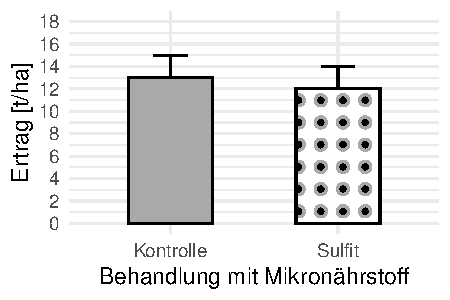
\includegraphics[width=\maxwidth]{img/mc-testing-ttest-02-1} 

}







\begin{enumerate}
\item [\textbf{A} \msquare] Die Barplots deuten auf keinen signifikanten Unterschied. Der Effekt liegt vermutlich bei -7. Wir müssen aber einen Posthoc-Test rechnen um den Effekt wirklich bestimmen zu können.
\item [\textbf{B} \msquare] Die Barplots deuten auf kein signifikanten Unterschied. Der Effekt liegt vermutlich bei -7.
\item [\textbf{C} \msquare] Nach Betrachtung des Barplots liegt kein signifikanter Unterschied vor. Der Effekt kann nicht bei einem t-Test aus Barplots bestimmt werden.
\item [\textbf{D} \msquare] Die Barplots deuten auf einen signifikanten Unterschied. Der Effekt liegt vermutlich bei -7 unter einer groben Abschätzung.
\item [\textbf{E} \msquare] Die Barplots deuten auf einen signifikanten Unterschied. Der Effekt liegt vermutlich bei -7 unter einer groben Abschätzung. Wir müssen aber eine ANOVA rechnen um den Effekt wirklich bestimmen zu können.
\end{enumerate}

\section{Aufgabe \hfill (2 Punkte)}




In Ihrer Abschlussarbeit betrachten Sie die Effekte von einer Behandlung vor und nach der Gabe eines Vitamins. Sie müssen einen gepaarten t-Test rechnen. Welche Aussage ist richtig?



\begin{enumerate}
\item [\textbf{A} \msquare] Der gepaarte t-Test wird genutzt, wenn die Differenzen der Beobachtungen verbunden sind und wir dadurch die Unabhäängigkeit nicht mehr vorliegen haben.
\item [\textbf{B} \msquare] Abhängige Beobachtungen müssen gesondert in einem gepaarten t-Test modelliert werden. Wenn wiederholt an dem gleichen Tier oder Pflanze gemessen wird, dann bilden wir den Quotienten zwischen den beiden Zeitpunkten. Auf den Quotienten rechnen wir den gepaarten t-Test.
\item [\textbf{C} \msquare] Beim gepaarten t-Test kombinieren wir die Vorteile des Student t-Test für Varianzhomogenität mit den Vorteilen des Welch t-Test für Varianzheterogenität. Wir bilden dafür die Differenz der Einzelbeobachtungen.
\item [\textbf{D} \msquare] Abhängige Beobachtungen müssen gesondert in einem gepaarten t-Test modelliert werden. Wenn wiederholt an dem gleichen Tier oder Pflanze gemessen wird, dann bilden wir die Differenz zwischen den beiden Zeitpunkten. Auf den Differenzen rechnen wir den gepaarten t-Test.
\item [\textbf{E} \msquare] Der gepaarte t-Test wird gerechnet, wenn die Beobachtungen abhängig voneinander sind. Wir messen jede Beobachtung nur einmal und berechnen dann die Differenz zu dem Mittel der anderen Beobachtungen.
\end{enumerate}

\section{Aufgabe \hfill (2 Punkte)}



Sie führen paarweise t-Tests für alle Vergleiche der verschiedenen Rapssorten in Ihrem Experiment durch. Nach der Adjustierung für multiples Testen ist kein p-Wert unter der $\alpha$-Schwelle. Ihr Experiment beinhaltet vier Rapssorten und eine ANOVA ergibt $p = 0.049$ für den Ertrag. Sie schauen sich auch die rohen, unadjustierten p-Werte an und finden hier als niedrigsten p-Wert $p_{3-2} = 0.053$. Welche Aussage ist richtig?




\begin{enumerate}
\item [\textbf{A} \msquare] Hier kommt der Effekt der stiegenden Fallzahl auf die Anzahl an signifikante Ergebnisse zu tragen. Da die ANOVA auf mehr Fallzahl testet als die einzelnen paarweisen t-Tests, kann die ANOVA leichter einen signifikanten Unterscheid nachweisen. Die p-Werte sind immer etwas kleiner als bei den t-Tests.
\item [\textbf{B} \msquare] Die adjustierten p-Werte deuten in die richtige Richtung. Zusammen mit den nicht signifikanten rohen p-Werten ist von einem Fehler in der ANOVA auszugehen.
\item [\textbf{C} \msquare] Das Beispiel kann so nicht auftreten, da die ANOVA und die t-Tests algorithmisch miteinander verschränkt sind.
\item [\textbf{D} \msquare] Es gibt einen Fehler in der Varianzstruktur. Daher kann die ANOVA nicht richtig sein und paarweise t-Tests liefern das richtige Ergebnis.
\item [\textbf{E} \msquare] Das ist kein Wunder. Die ANOVA testet nicht auf der gesamten Fallzahl und die paarweisen t-Tests gewinnen immer eine oder mehr Gruppen als Fallzahl dazu. Mit steigender Fallzahl sind mehr signifikante Unterschiede zu erwarten. Die p-Werte unterscheiden sich numerisch auch kaum.
\end{enumerate}
    
% -----------------------------------------------------------------------
\clearpage
% -----------------------------------------------------------------------
\part{Deskriptive Statistik \& Explorative Datenanalyse}
% -----------------------------------------------------------------------

\section{Aufgabe \hfill (7 Punkte)}

\textit{Geben Sie grundsätzlich Formeln und Rechenweg zur Lösung der Teilaufgaben mit an!} \\[1Ex]
 

 
%% --------------------------------------------------------------------
\begin{minipage}[t]{0.5\textwidth}

\includegraphics[width = 1.3cm]{/Users/kruppajo/work/GitHub/exam/avatare/Nilufar.png}
\end{minipage}
\begin{minipage}[t]{0.5\textwidth}
\hfill
\href{https://youtu.be/t0WYa_LVc5o}{
\includegraphics[width = 2cm]{img/youtube}}\\[1Ex]
\end{minipage}
\vspace{1ex}
%% --------------------------------------------------------------------



Nilufar steht vor einem ersten Problem, denn wenn es nach ihrer Betreuerin geht, soll sie in einem einer Klimakammer Erdbeeren auswertet. Soweit eigentlich alles passend. Die Behandlung werden verschiedene Substrattypen ($torf$, $40p60n$ und $70p30n$) sein. In ihrer Exceldatei wird sie den Messwert ($Y$) \textit{Trockengewicht} als \textit{drymatter} aufnehmen. Vorab soll Nilufar aber eimal die folgenden Barplots ihrer Betreuerin nachbauen, damit sie den \Rlogo Code schonmal für später vorliegen hat. Damit geht das Problem schon los.



{\centering 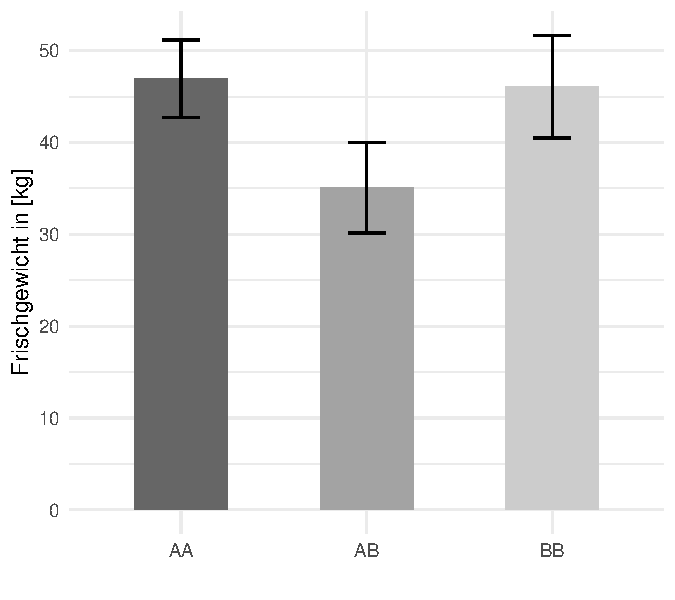
\includegraphics[width=\maxwidth]{img/barplot-02-1} 

}




Leider kennt sich Nilufar mit der Erstellung von Barplots in \Rlogo nicht aus. Deshalb braucht sie bei der Visualisierung Ihre Hilfe!

\begin{enumerate}
\item Erstellen Sie eine Tabelle mit den statistischen Maßzahlen aus der
  obigen Abbildung der drei Barplots! \textit{Beachten Sie die korrekte
    Darstellungsform der statistischen Maßzahlen!} \textbf{(3 Punkte)}
\item Erstellen Sie einen beispielhaften Datensatz, aus dem die drei
  Barplots \textit{möglicherweise} erstellt wurden, im \Rlogo üblichen Format! \textbf{(2 Punkte)}
\item Erwarten Sie einen Unterschied zwischen den Behandlungen? Begründen
  Sie Ihre Antwort! \textbf{(2 Punkte)}
\end{enumerate} 
\clearpage
% -----------------------------------------------------------------------

\section{Aufgabe \hfill (7 Punkte)}

\textit{Geben Sie grundsätzlich Formeln und Rechenweg zur Lösung der Teilaufgaben mit an!} \\[1Ex]
 

 
%% --------------------------------------------------------------------
\begin{minipage}[t]{0.5\textwidth}

\includegraphics[width = 1.3cm]{/Users/kruppajo/work/GitHub/exam/avatare/Nilufar.png}
\end{minipage}
\begin{minipage}[t]{0.5\textwidth}
\hfill
\href{https://youtu.be/vXnLttRL_VI}{
\includegraphics[width = 2cm]{img/youtube}}\\[1Ex]
\end{minipage}
\vspace{1ex}
%% --------------------------------------------------------------------



Anschauen, was andere vor einem gemacht haben, ist eine Möglichkeit schnell ans Ziel zu gelangen. Deshalb hat sich Nilufar viele Poster in der Fakultät angeschaut und ist zum Schluß gekommen, dass Barplots eine häufig genutzte Abbildung sind. Nilufar soll nun in ihrem Projektbericht Lauch untersuchen. Die Behandlung in ihrem Projektbericht sind verschiedene Genotypen ($AA$, $AB$ und $BB$). Erhoben wurden von Nilufar als Outcome ($Y$) \textit{Proteingehalt} benannt als \textit{protein} in ihrer Exceldatei. Erwartungsgemäß erhält sie von ihrer Betreuerin den Auftrag die erhobenen Daten als Barplots darzustellen. Dann kann Nilufar auch schonmal abschätzen, was bei einem statistischen Test rauskommen könnte.

\begin{table}[!h]
\centering
\begin{tabular}{cc}
\toprule
treatment & protein\\
\midrule
BB & 34.7\\
BB & 35.6\\
BB & 36.5\\
AA & 39.2\\
AB & 44.6\\
\addlinespace
AA & 35.7\\
AB & 37.3\\
AA & 50.5\\
BB & 42.5\\
AA & 40.4\\
\addlinespace
AB & 38.2\\
AA & 45.2\\
\bottomrule
\end{tabular}
\end{table}



Leider kennt sich Nilufar mit der Erstellung von Barplots nicht aus. Deshalb braucht sie bei der Visualisierung Ihre Hilfe!

\begin{enumerate}
\item Zeichnen Sie in \textit{einer} Abbildung die Barplots für die
  Behandlung von Lauch! Beschriften Sie die Achsen entsprechend!
  \textbf{(4 Punkte)}
\item Beschriften Sie \textit{einen} Barplot mit den gängigen
  statistischen Maßzahlen! \textbf{(2 Punkte)}
\item Wenn Sie \textit{keinen Effekt} zwischen den Behandlungen von
  Lauch erwarten würden, wie sehen dann die Barplots aus?
  \textit{Antworten Sie mit einer Skizze der Barplots!}
  \textbf{(1 Punkt)}
\end{enumerate} 
\clearpage
% -----------------------------------------------------------------------

\section{Aufgabe \hfill (9 Punkte)}

\textit{Geben Sie grundsätzlich Formeln und Rechenweg zur Lösung der Teilaufgaben mit an!} \\[1Ex]
 

 
%% --------------------------------------------------------------------
\begin{minipage}[t]{0.5\textwidth}

\includegraphics[width = 1.3cm]{/Users/kruppajo/work/GitHub/exam/avatare/Alex.png}
\end{minipage}
\begin{minipage}[t]{0.5\textwidth}
\hfill
\href{https://youtu.be/Xf0yE-o7bEU}{
\includegraphics[width = 2cm]{img/youtube}}\\[1Ex]
\end{minipage}
\vspace{1ex}
%% --------------------------------------------------------------------



Boxplots sind bedeutend in der Darstellung von wissenschaftlichen Ergebnissen. Leider hat sich Alex nicht gemerkt, welche statistischen Maßzahlen für einen Boxplot erhoben werden müssen. Das ist in soweit doof, da nach seiner Betreuerin erstmal ein Boxplot nachgebaut werden soll, bevor es mit seiner Hausarbeit losgeht. Anhand von Boxplots lässt sich eine Aussage über die Normalverteilung von $Y$ treffen. Dann hat er schonmal den \Rlogo Code vorliegen und nachher geht dann alles schneller. Die Behandlung für Lauch werden verschiedene Lichtstufen ($none$, $200lm$ und $600lm$) sein. Erfasst wird als Endpunkt ($Y$) \textit{Proteingehalt}. Alex soll dann \textit{protein} in seiner Exceldatei eintragen.



{\centering 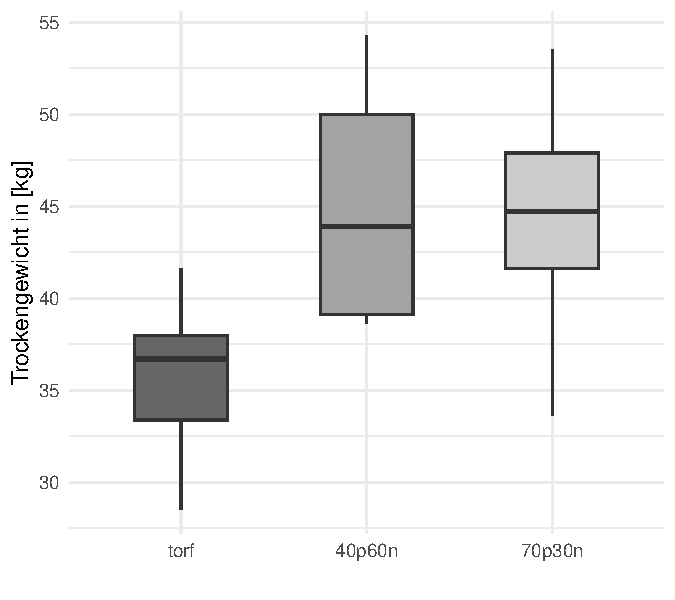
\includegraphics[width=\maxwidth]{img/boxplot-02-zer-1} 

}




Leider kennt sich Alex mit der Erstellung von Boxplots in \Rlogo nicht aus. Deshalb braucht er bei der Visualisierung Ihre Hilfe!

\begin{enumerate}
\item Erstellen Sie eine Tabelle mit den statistischen Maßzahlen aus der
  obigen Abbildung der drei Boxplots! \textit{Beachten Sie die korrekte
    Darstellungsform der statistischen Maßzahlen!} \textbf{(3 Punkte)}
\item Beschriften Sie \textit{einen} der Boxplots mit den gängigen
  statistischen Maßzahlen! \textbf{(2 Punkte)}
\item Erstellen Sie einen beispielhaften Datensatz, aus dem die drei
  Boxplots \textit{möglicherweise} erstellt wurden, im \Rlogo üblichen Format! \textbf{(2 Punkte)}
\item Erwarten Sie einen Unterschied zwischen den Behandlungen? Begründen
  Sie Ihre Antwort! \textbf{(2 Punkte)}
\end{enumerate} 
\clearpage
% -----------------------------------------------------------------------

\section{Aufgabe \hfill (9 Punkte)}

\textit{Geben Sie grundsätzlich Formeln und Rechenweg zur Lösung der Teilaufgaben mit an!} \\[1Ex]
 

 
%% --------------------------------------------------------------------
\begin{minipage}[t]{0.5\textwidth}

\includegraphics[width = 1.3cm]{/Users/kruppajo/work/GitHub/exam/avatare/Jonas.png}
\end{minipage}
\begin{minipage}[t]{0.5\textwidth}
\hfill
\href{https://youtu.be/0xc0jIPeiyw}{
\includegraphics[width = 2cm]{img/youtube}}\\[1Ex]
\end{minipage}
\vspace{1ex}
%% --------------------------------------------------------------------



Anschauen, was andere vor einem gemacht haben, ist eine Möglichkeit schnell ans Ziel zu gelangen. Deshalb hat sich Jonas viele Poster in der Fakultät angeschaut und ist zum Schluß gekommen, dass Boxplots eine häufig genutzte Abbildung sind. Jonas soll nun in seiner Abschlussarbeit Kartoffeln untersuchen. Die Behandlung in seiner Abschlussarbeit sind verschiedene Genotypen ($AA$ und $BB$). Erhoben wurden von Jonas als Endpunkt ($Y$) \textit{Frischegewicht} benannt als \textit{freshmatter} in seiner Exceldatei. Erwartungsgemäß erhält er von seiner Betreuerin den Auftrag die erhobenen Daten als Boxplots darzustellen. Dann kann Jonas auch schonmal abschätzen, was bei einem statistischen Test rauskommen könnte. Darüber hinaus kann Jonas anhand Boxplots eine Aussage über die Normalverteilung von $Y$ treffen.

\begin{table}[!h]
\centering
\begin{tabular}{cc}
\toprule
treatment & drymatter\\
\midrule
AA & 43.6\\
BB & 31.2\\
BB & 22.7\\
AA & 34.8\\
AA & 38.2\\
\addlinespace
AA & 36.9\\
BB & 28.7\\
BB & 20.5\\
AA & 38.2\\
AA & 40.8\\
\addlinespace
BB & 23.2\\
AA & 42.9\\
BB & 23.8\\
AA & 42.6\\
BB & 28.6\\
\bottomrule
\end{tabular}
\end{table}



Leider kennt sich Jonas mit der Erstellung von Boxplots nicht aus. Deshalb braucht er bei der Visualisierung Ihre Hilfe!

\begin{enumerate}
\item Zeichnen Sie in \textit{einer} Abbildung die beiden Boxplots für die zwei Behandlungen von Kartoffeln! Beschriften Sie die Achsen entsprechend! \textbf{(5 Punkte)} 
\item Wie ist Ihr Vorgehen, wenn Sie eine \textit{gerade} Anzahl an
  Beobachtungen pro Gruppe haben? \textbf{(1 Punkt)}
\item Beschriften Sie \textit{einen} der beiden Boxplots mit den gängigen
  statistischen Maßzahlen! \textbf{(2 Punkte)}
\item Wenn Sie \textit{keinen Effekt} zwischen den Behandlungen von
  Kartoffeln erwarten würden, wie sehen dann die beiden Boxplots aus?
  \textit{Antworten Sie mit einer Skizze der Boxplots!}
  \textbf{(1 Punkt)}
\end{enumerate} 
\clearpage
% -----------------------------------------------------------------------

\section{Aufgabe \hfill (8 Punkte)}

\textit{Geben Sie grundsätzlich Formeln und Rechenweg zur Lösung der Teilaufgaben mit an!} \\[1Ex]
 

 
%% --------------------------------------------------------------------
\begin{minipage}[t]{0.5\textwidth}

\includegraphics[width = 1.3cm]{/Users/kruppajo/work/GitHub/exam/avatare/Tina.png}
\end{minipage}
\begin{minipage}[t]{0.5\textwidth}
\hfill
\href{https://youtu.be/aXvxGC4YLqk}{
\includegraphics[width = 2cm]{img/youtube}}\\[1Ex]
\end{minipage}
\vspace{1ex}
%% --------------------------------------------------------------------



In ihrer Abschlussarbeit möchte Tina gerne die Daten aus einem Stallexperiment mit Schweinen in einem Histogramm darstellen. Das Histogramm erlaubt ihr dabei Rückschlüsse auf die Verteilung über das Outcome ($Y$) zu treffen. In seinem Experiment hat Tina die Anzahl an gedrehten Haaren pro $cm^2$ gezählt.

\begin{center}
Die Anzahl an gedrehten Haaren pro $cm^2$: 6, 5, 1, 3, 5, 3, 4, 6, 3, 2, 1, 2, 2, 4, 5, 1, 4, 2, 3, 2, 5, 3, 3, 6, 6, 2, 1, 8, 7, 3, 4, 2, 3, 5, 3, 5
\end{center}

Leider kennt sich Tina mit der Erstellung von Histogrammen überhaupt nicht aus. Deshalb braucht sie bei der Erstellung Ihre Hilfe!

\begin{enumerate}
\item Zeichen Sie ein Histogramm um die Verteilung der Daten zu visualisieren! (\textbf{3 Punkte})
\item Beschriften Sie die Achsen der Abbildung! (\textbf{2 Punkte})
\item Ergänzen Sie die absoluten und relativen Häufigkeiten in der
  Abbildung! \textbf{(1 Punkt)}
\item Berechnen Sie aus den Daten die \textit{Wahrscheinlichkeit}
  mehr als die Anzahl 5 zu beobachten! \textbf{(1
    Punkt)}
\item Berechnen Sie aus den Daten die \textit{Chance} mehr
  als die Anzahl 5 zu beobachten! \textbf{(1 Punkt)}
\end{enumerate}

 
\clearpage
% -----------------------------------------------------------------------

\section{Aufgabe \hfill (8 Punkte)}

\textit{Geben Sie grundsätzlich Formeln und Rechenweg zur Lösung der Teilaufgaben mit an!} \\[1Ex]
 

 
%% --------------------------------------------------------------------
\begin{minipage}[t]{0.5\textwidth}

\includegraphics[width = 1.3cm]{/Users/kruppajo/work/GitHub/exam/avatare/Steffen.png}
\end{minipage}
\begin{minipage}[t]{0.5\textwidth}
\hfill
\href{https://youtu.be/ORHSPTCdfeY}{
\includegraphics[width = 2cm]{img/youtube}}\\[1Ex]
\end{minipage}
\vspace{1ex}
%% --------------------------------------------------------------------



In seiner Abschlussarbeit möchte Steffen gerne die Daten aus einem Leistungssteigerungsversuch mit Schweinen in einem Histogramm darstellen. Das Histogramm erlaubt ihm dabei Rückschlüsse auf die Verteilung über den Endpunkt ($Y$) zu treffen. In seinem Experiment hat Steffen die mittlere Anzahl an weißen Blutkörperchen gezählt.

\begin{center}
Die mittlere Anzahl an weißen Blutkörperchen: 12.1, 13.9, 10.4, 9.9, 10.4, 10.5, 10, 13.9, 8.8, 9.5, 8.3, 8, 10.7, 8.9, 9.4, 11, 6.1, 7.7, 11.6, 10.7, 9, 9.3
\end{center}

Leider kennt sich Steffen mit der Erstellung von Histogrammen überhaupt nicht aus. Deshalb braucht er bei der Erstellung Ihre Hilfe!

\begin{enumerate}
\item Zeichen Sie ein Histogramm um die Verteilung der Daten zu
  visualisieren! (\textbf{3 Punkte})
 \item Erläutern Sie Ihr Vorgehen um ein Histogramm für kontinuierliche
  Daten zu zeichnen!  (\textbf{2 Punkte})
\item Beschriften Sie die Achsen der Abbildung! (\textbf{2 Punkte})
\item Ergänzen Sie die relativen Häufigkeiten in der Abbildung! \textbf{(1
    Punkt)}  
\end{enumerate}

 
\clearpage
% -----------------------------------------------------------------------

\section{Aufgabe \hfill (10 Punkte)}

\textit{Geben Sie grundsätzlich Formeln und Rechenweg zur Lösung der Teilaufgaben mit an!} \\[1Ex]
 

 
%% --------------------------------------------------------------------
\begin{minipage}[t]{0.5\textwidth}

\includegraphics[width = 1.3cm]{/Users/kruppajo/work/GitHub/exam/avatare/Mark.png}
\end{minipage}
\begin{minipage}[t]{0.5\textwidth}
\hfill
\href{https://youtu.be/VAqiUdV4WQ0}{
\includegraphics[width = 2cm]{img/youtube}}\\[1Ex]
\end{minipage}
\vspace{1ex}
%% --------------------------------------------------------------------




Mark möchte gerne den Zusammenhang zwischen mittlerer Eisenkonzentration [Fe/ml] und Protein/Fettrate [\%/kg] im Kontext von Schweinen herausfinden. Hierfür hat Mark ein Kreuzungsexperiment in der Uckermark durchgeführt. Nach einigen unvorgesehenen Ereignissen hat er es geschafft folgende Datentabelle zu erstellen. Nun stellt sich die Frage für ihn, ob es überhaupt einen Zusammenhang zwischen den gemessenen Variablen gibt. Deshalb möchte Mark als erstes eine explorative Datenanalyse durchführen.

\begin{table}[!h]
\centering
\begin{tabular}{cc}
\toprule
Protein/Fettrate [\%/kg] & Mittlerer Eisenkonzentration [Fe/ml]\\
\midrule
23.8 & 33.4\\
18.5 & 23.0\\
24.7 & 28.9\\
20.4 & 27.1\\
16.3 & 20.7\\
\addlinespace
20.7 & 29.7\\
18.3 & 26.5\\
21.7 & 27.6\\
22.8 & 30.8\\
15.7 & 24.5\\
\bottomrule
\end{tabular}
\end{table}



Leider kennt sich Mark mit der Erstellung einer explorativen Datenanalyse für kontinuierliche Daten überhaupt nicht aus. Deshalb braucht er bei der Erstellung Ihre Hilfe!

\begin{enumerate}
\item Erstellen Sie eine Visualisierung für die Datentabelle. Beschriften Sie
  die Achsen entsprechend! \textbf{(4 Punkte)}
\item Schätzen Sie eine Gerade durch die Punkte! \textbf{(1 Punkt)}
\item Beschriften Sie die Gerade mit den gängigen statistischen Maßzahlen! Geben Sie die numerischen Zahlenwerte mit an! \textbf{(3 Punkte)}
\item Wenn \textit{kein} Effekt von $x$ auf $y$ vorhanden wäre, wie würde die Gerade verlaufen und welche Werte würden die statistischen Maßzahlen annehmen? \textbf{(2 Punkt)}
\end{enumerate} 
\clearpage
% -----------------------------------------------------------------------

\section{Aufgabe \hfill (10 Punkte)}

\textit{Geben Sie grundsätzlich Formeln und Rechenweg zur Lösung der Teilaufgaben mit an!} \\[1Ex]
 

 
%% --------------------------------------------------------------------
\begin{minipage}[t]{0.5\textwidth}

\includegraphics[width = 1.3cm]{/Users/kruppajo/work/GitHub/exam/avatare/Jessica.png}
\end{minipage}
\begin{minipage}[t]{0.5\textwidth}
\hfill
\href{https://youtu.be/t_1KL77mfmg}{
\includegraphics[width = 2cm]{img/youtube}}\\[1Ex]
\end{minipage}
\vspace{1ex}
%% --------------------------------------------------------------------



'Uff!', denkt sich Jessica. Jetzt hat sie doch tatsächlich zwei kategoriale Variablen in ihrer Abschlussarbeit gemessen. Zum einen die Behandlung Außenklimakontakt [ja/nein] und zum anderen die Messung Gewichtszuwachs erreicht [ja/nein] im Kontext von Schweinen. Hierfür hat sie ein Stallexperiment im Wendland durchgeführt. Jetzt möchte Jessica die Daten einmal in einer explorativen Datenanalyse darstellen. Danach kann sie dann über den passenden statistischen Test nachdenken. Dabei unterstützt ihre Betreuerin diesen Ansatz bevor es in der Datenanalyse weiter geht.



\vspace{1Ex}

\begin{center}
\begin{minipage}[t]{0.45\textwidth}
\small
\begin{center}

\begin{tabular}{p{2.5cm}p{2.5cm}p{2.5cm}p{2.5cm}}
\toprule
Gewichtszuwachs erreicht & Außenklimakontakt\\
\midrule
nein & ja\\
nein & ja\\
nein & nein\\
nein & ja\\
ja & ja\\
\addlinespace
nein & ja\\
ja & nein\\
nein & ja\\
ja & nein\\
nein & ja\\
\addlinespace
ja & nein\\
nein & ja\\
ja & nein\\
nein & ja\\
ja & nein\\
\addlinespace
nein & nein\\
ja & ja\\
\bottomrule
\end{tabular}


\end{center}
\end{minipage}
\begin{minipage}[t]{0.45\textwidth}
\small
\begin{center}

\begin{tabular}{p{2.5cm}p{2.5cm}p{2.5cm}p{2.5cm}}
\toprule
Gewichtszuwachs erreicht & Außenklimakontakt\\
\midrule
ja & nein\\
ja & nein\\
ja & nein\\
nein & nein\\
ja & nein\\
\addlinespace
ja & ja\\
ja & ja\\
nein & ja\\
nein & nein\\
ja & nein\\
\addlinespace
ja & nein\\
nein & ja\\
nein & ja\\
ja & ja\\
ja & nein\\
\addlinespace
nein & ja\\
ja & nein\\
\bottomrule
\end{tabular}


\end{center}
\end{minipage}
\end{center}

\vspace{2Ex}

Leider kennt sich Jessica mit der Erstellung einer explorativen Datenanalyse für kategoriale Daten überhaupt nicht aus. Deshalb braucht sie bei der Erstellung Ihre Hilfe!

\begin{enumerate}
\item Stellen Sie den Zusammenhang zwischen den beiden kategorialen Variablen in einer zusammenfassenden Tabelle dar! \textbf{(3 Punkte)}
\item Visualisieren Sie den Zusammenhang zwischen den beiden kategorialen Variablen! \textbf{(3 Punkte)}
\item Berechnen Sie die Verhältnisse in der Visualisierung! Welche Annahme haben Sie getroffen? \textbf{(2 Punkte)}
\item Wenn \textit{ein} Effekt von der Behandlung vorliegen würde, wie würde die Tabelle und die Visualisierung aussehen? \textbf{(2 Punkt)}
\end{enumerate} 
\clearpage
% -----------------------------------------------------------------------

\section{Aufgabe \hfill (10 Punkte)}

\textit{Geben Sie grunds{\"a}tzlich Formeln und Rechenweg zur L{\"o}sung der
  Teilaufgaben mit an!} \\[1Ex]

%% --------------------------------------------------------------------
\hfill\href{https://youtu.be/Op-gjzASH9I}{
\includegraphics[width =
  2cm]{img/youtube}}\\[1Ex]
%% --------------------------------------------------------------------



\begin{enumerate}
\item Zeichnen Sie {\"u}ber die untenstehenden Boxplots die entsprechende
  zugeh{\"o}rige Verteilung! \textbf{(3 Punkte)} 
\item Zeichnen Sie unter die untenstehenden Boxplots die entsprechende
  zugeh{\"o}rige Beobachtungen als Stiche! \textbf{(3 Punkte)}
\item Wieviel Prozent der Beobachtungen fallen in das IQR? Erg{\"a}nzen Sie die
  Abbildung entsprechend um den Bereich! \textbf{(2 Punkte)}
\item Wieviel Prozent der Beobachtungen fallen in $\pm 1s$ unter
  der Annahme einer Normalverteilung?  \textit{Wenn m{\"o}glich}, erg{\"a}nzen Sie
  die Abbildung entsprechend um den Bereich! \textbf{(2 Punkte)}
\end{enumerate}




{\centering 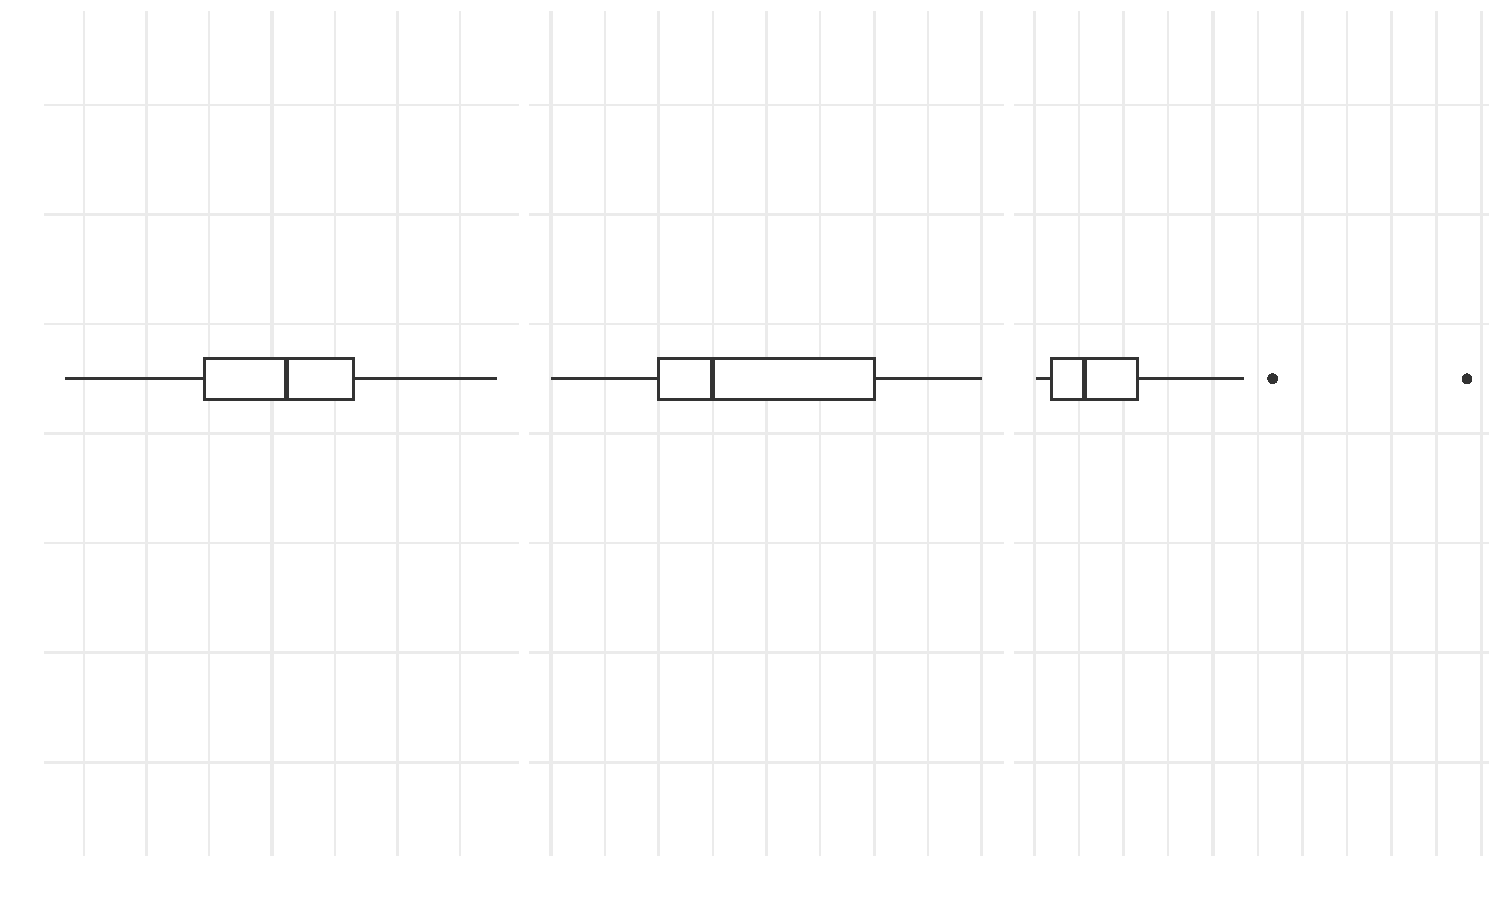
\includegraphics[width=\maxwidth]{img/desc-stat-11-1} 

}




 
\clearpage
% -----------------------------------------------------------------------

\section{Aufgabe \hfill (9 Punkte)}

\textit{Geben Sie grunds{\"a}tzlich Formeln und Rechenweg zur L{\"o}sung der
  Teilaufgaben mit an!} \\[1Ex]

%% --------------------------------------------------------------------
\hfill\href{https://youtu.be/ZrJhn2wPbq4}{
\includegraphics[width =
  2cm]{img/youtube}}\\[1Ex]
%% --------------------------------------------------------------------



\begin{enumerate}
\item Skizieren Sie $3$ Normalverteilungen \textit{in einer
    Abbildung} mit $\bar{y}_1 \neq \bar{y}_2 \neq \bar{y}_3$ und $s_1 \neq s_2 \neq s_3$! \textbf{(3 Punkte)}
\item Beschriften Sie die Normalverteilungen mit den entsprechenden
  Parametern! \textbf{(2 Punkte)}
\item Erg{\"a}nzen Sie die Bereiche in der 68\% und 95\% der Beobachtungen
  fallen! Beschriften Sie die Grenzen der Bereiche mit der statistischen Ma{\ss}zahl! \textbf{(2 Punkte)}
\item Liegt Varianzhomogenit{\"a}t oder Varianzheterogenit{\"a}t vor? Begr{\"u}nden Sie
  Ihre Antwort! \textbf{(2 Punkte)}
\end{enumerate}

 
\clearpage
% -----------------------------------------------------------------------

\section{Aufgabe \hfill (9 Punkte)}

\textit{Geben Sie grunds{\"a}tzlich Formeln und Rechenweg zur L{\"o}sung der
  Teilaufgaben mit an!} \\[1Ex]

%% --------------------------------------------------------------------
\hfill\href{https://youtu.be/MiD42k4l5Ag}{
\includegraphics[width =
  2cm]{img/youtube}}\\[1Ex]
%% --------------------------------------------------------------------



\begin{enumerate}
\item Skizieren Sie in die unten stehenden, freien Abbildungen die
  Verteilungen, die sich nach der Abbildungs{\"u}berschrift ergeben! \textbf{(6
    Punkte)}
\item Beschriften Sie die Achsen der Abbildungen entsprechend! \textbf{(1
    Punkt)}
\item Achten Sie auf die entsprechende Skalierung der beiden Verteilungen
  in den Abbildungen! \textbf{(2 Punkte)}
\end{enumerate}



{\centering 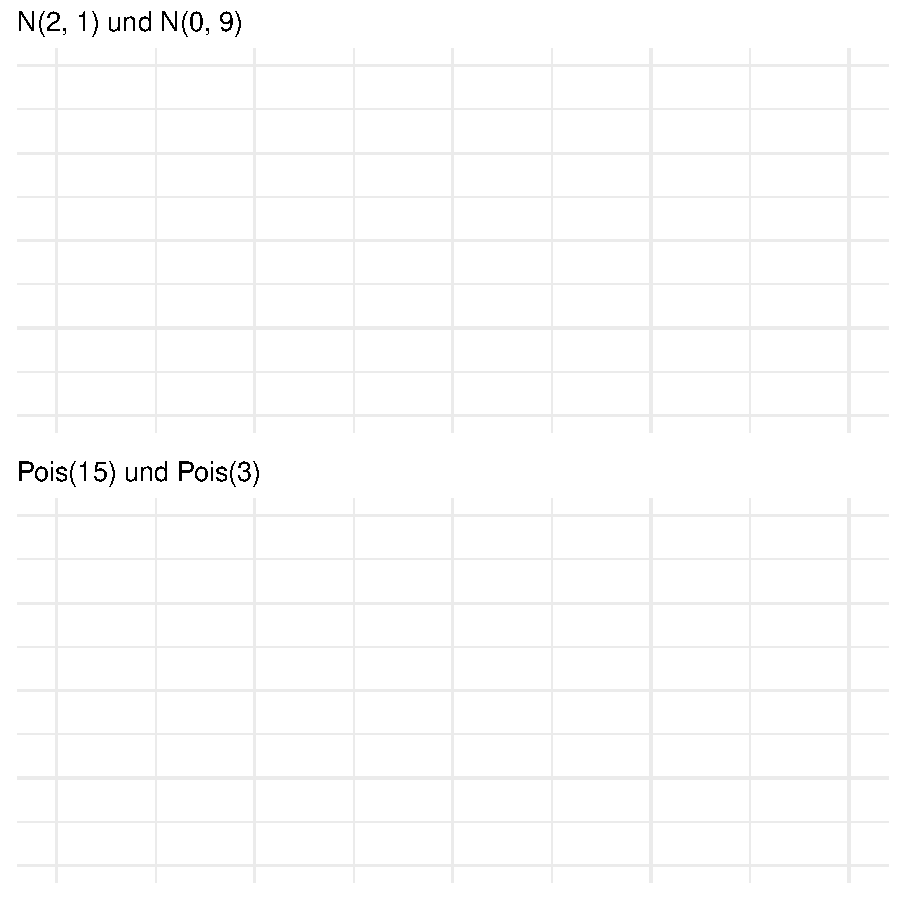
\includegraphics[width=\maxwidth]{img/histogram-01-1} 

}



 
\clearpage
% -----------------------------------------------------------------------

\section{Aufgabe \hfill (8 Punkte)}

\textit{Geben Sie grunds{\"a}tzlich Formeln und Rechenweg zur L{\"o}sung der
  Teilaufgaben mit an!} \\[1Ex]

%% --------------------------------------------------------------------
\hfill\href{https://youtu.be/oMdtYbDInYE}{
\includegraphics[width =
  2cm]{img/youtube}}\\[1Ex]
%% --------------------------------------------------------------------

Sie haben folgende Zahlenreihe $y$ vorliegen
$y = \{17, 17, 20, 14, 16, 15\}$.

\begin{enumerate}
\item Visualisieren Sie den Mittelwert von $y$ in der untenstehenden
  Abbildung! \textbf{(4 Punkte)}
\item Beschriften Sie die $Y$ und $X$-Achse entsprechend! \textbf{(2 Punkte)}
\item F{\"u}r die Berechnung der Varianz wird der Abstand der einzelnen Werte $y_i$
  zum Mittelwert $\bar{y}$ quadriert. Warum muss der Abstand, $y_i -
  \bar{y}$, in der Varianzformel quadriert werden?
  Erkl{\"a}ren Sie den Zusammenhang unter Ber{\"u}cksichtigung der Abbildung!
  \textbf{(2 Punkte)}  
\end{enumerate}



{\centering 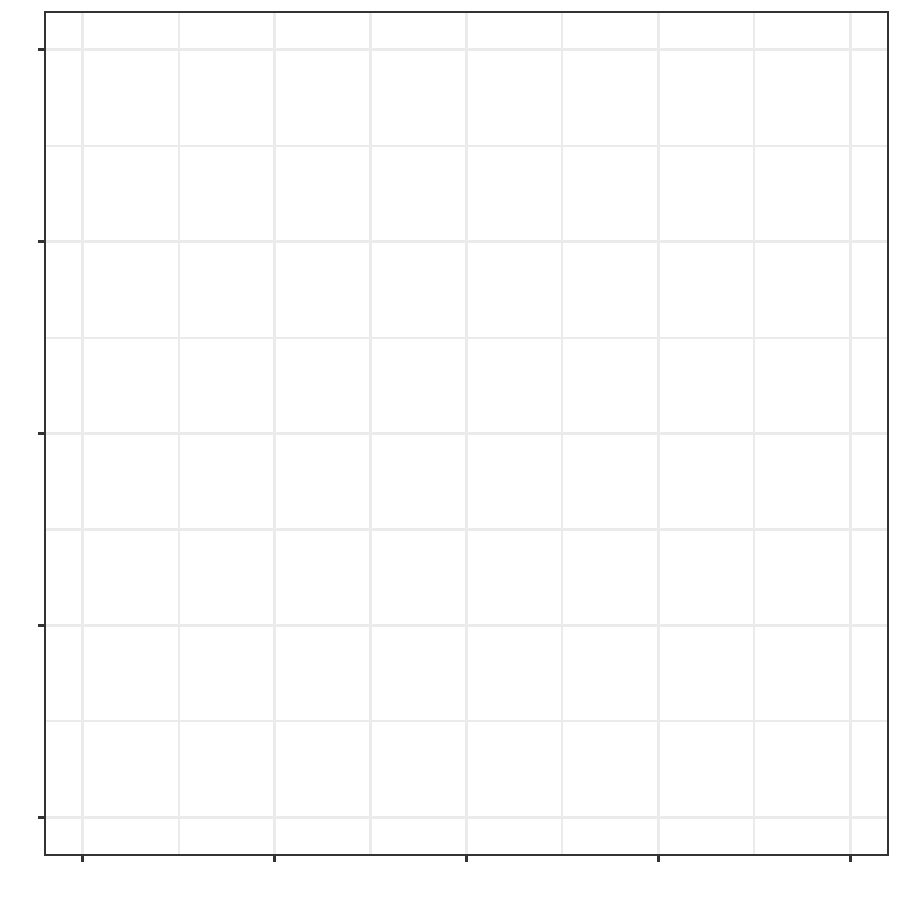
\includegraphics[width=\maxwidth]{img/desc-01-1} 

}


 
\clearpage
% -----------------------------------------------------------------------
\part{Statistisches Testen \& statistische Testtheorie}
% -----------------------------------------------------------------------  

\section{Aufgabe \hfill (9 Punkte)}

%% --------------------------------------------------------------------
\hfill\href{https://youtu.be/aHVYuFKTqZs}{
\includegraphics[width =
  2cm]{img/youtube}}\\[1Ex]
%% --------------------------------------------------------------------

Grundlage des statistischen Testen ist das Verst{\"a}ndnis von der
Grundgesamtheit (eng. \textit{population} oder \textit{ground truth}) und
der experimentellen Stichprobe (eng. \textit{sample}). 

\begin{enumerate}
\item Nennen Sie das statistische Verfahren und zwei konkrete Beispiele zur
  Durchf{\"u}hrung um von einer Grundgesamtheit auf eine Stichprobe zu
  gelangen! \textbf{(3 Punkte)}
\item Erkl{\"a}ren Sie den Zusammenhang zwischen Stichprobe und Grundgesamtheit
  an einem Schaubild! Beschriften Sie das Schaubild entsprechend!
  \textit{Nutzen Sie hierf{\"u}r als Veranschaulichung die K{\"o}rpergr{\"o}{\ss}e von
    M{\"a}nnern oder Frauen aus den Gummib{\"a}rchendaten!}  \textbf{(3 Punkte)}
\item Erweitern Sie das Schaubild um die Entstehung von $Pr(D|H_0)$!
  \textit{Nutzen Sie hierf{\"u}r als Veranschaulichung zus{\"a}tzlich die
    Gruppierungsvariable "`Modul"' aus den Gummib{\"a}rchendaten!}  \textbf{(3
    Punkte)}
\end{enumerate} 
\clearpage
% -----------------------------------------------------------------------

\section{Aufgabe \hfill (9 Punkte)}

%% --------------------------------------------------------------------
\hfill\href{https://youtu.be/Ric8ne39DtI}{
\includegraphics[width =
  2cm]{img/youtube}}\\[1Ex]
%% --------------------------------------------------------------------




F{\"u}r ein besseres Verst{\"a}ndnis der statistischen Testtheorie, auch
Null-Ritual genannt, kann eine Visualisierung als Kreuztabelle genutzt werden.  

\begin{enumerate}
\item Tragen Sie folgende statistische Fachbegriffe zur statistischen
  Testtheorie korrekt eine selbst erstellte Kreuztabelle ein! \textbf{(3
    Punkte)}
  \begin{center}
  \begin{tabular}{cccc}
  $\beta$-Fehler & 20\% & H$_0$ falsch & H$_0$ abgelehnt \\
  \end{tabular}
  \end{center}
\item Erg{\"a}nzen Sie Ihre erstellte Kreuztabelle um vier weitere, passende
  Fachbegriffe zur statistischen Testtheorie! \textbf{(2 Punkte)}
\end{enumerate}

Die Entscheidungsfindung durch einen statistischen Test kann auch durch die
Analogie zu einem Feuermelder abgebildet werden. Dabei symbolisiert der
Feuermelder den statistischen Test und es soll getestet werden, ob ein Feuer
ausgebrochen ist.

\begin{enumerate}
  \setcounter{enumi}{2}    
\item In der Analogie des Feuermelders, wie lautet der $\alpha$-Fehler? \textbf{(1 Punkt)}
\item In der Analogie des Feuermelders, wie lautet der $\beta$-Fehler? \textbf{(1 Punkt)}
\item Wenn der Feuermelder einmal pro Tag messen w{\"u}rde, wie oft w{\"u}rde der
  Feuermelder mit einem $\alpha$ von 5\% in einem halben Jahr Alarm schlagen?
  Begr{\"u}nden Sie Ihre Antwort! \textbf{(2 Punkte)}
\end{enumerate}



 
\clearpage
% -----------------------------------------------------------------------

\section{Aufgabe \hfill (9 Punkte)}

\textit{Geben Sie grunds{\"a}tzlich Formeln und Rechenweg zur L{\"o}sung der
  Teilaufgaben mit an!} \\[1Ex]

%% --------------------------------------------------------------------
\hfill\href{https://youtu.be/32JjH1eyuTU}{
\includegraphics[width =
  2cm]{img/youtube}}\\[1Ex]
%% --------------------------------------------------------------------



Abgebildet ist die t-Verteilung unter der Anahme der G{\"u}ltigkeit der
Nullhypothese. \textit{Beachten Sie, dass im Folgenden keine
  numerisch korrekte Darstellung verlangt wird! Es gilt Erkennbarkeit vor
  Genauigkeit!}

\begin{enumerate}
\item Erg{\"a}nzen Sie eine beschriftete $x$-Achse! \textbf{(1 Punkt)}
\item Erg{\"a}nzen Sie "`$\bar{y}_1 = \bar{y}_2$"'! \textbf{(1 Punkt)} 
\item Erg{\"a}nzen Sie "`$A = 95\%$"'! \textbf{(1 Punkt)}
\item Zeichnen Sie $T_{\alpha=5\%}$ in die Abbildung! \textbf{(1 Punkt)} 
\item Zeichnen Sie das Signifikanzniveau $\alpha$ in die Abbildung! Begr{\"u}nden
  Sie Ihre Antwort! \textbf{(2 Punkte)} 
\item Zeichnen Sie $+T_{D}$ in die Abbildung! \textbf{(1
    Punkt)}
\item Zeichnen Sie einen signifikant p-Wert in die Abbildung! Begr{\"u}nden
  Sie Ihre Antwort! \textbf{(2 Punkte)}   
\end{enumerate}



{\centering 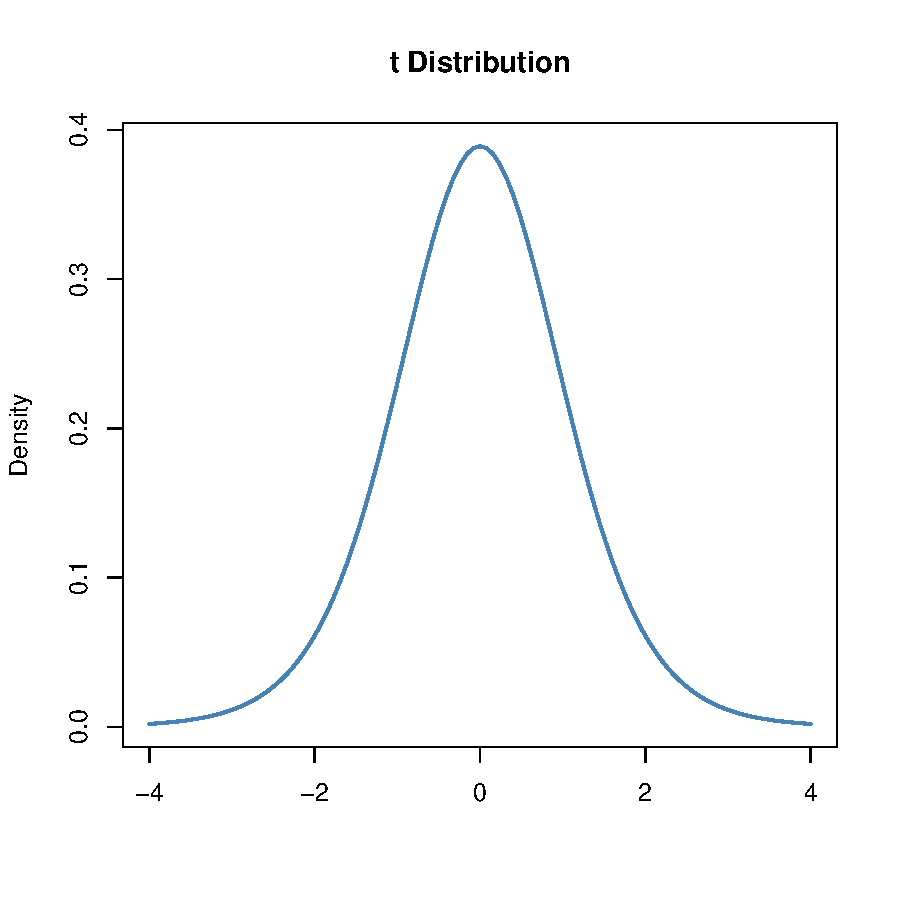
\includegraphics[width=\maxwidth]{img/statistisches-testen-3-1} 

}


 
\clearpage
% -----------------------------------------------------------------------

\section{Aufgabe \hfill (10 Punkte)}

%% --------------------------------------------------------------------
\hfill\href{https://youtu.be/CN_O4fYPbhs}{
\includegraphics[width =
  2cm]{img/youtube}}\\[1Ex]
%% --------------------------------------------------------------------



Sie rechnen einen t-Test f{\"u}r Gruppenvergleiche der Mittelwerte. Sie
sch{\"a}tzen den Unterschied zwischen dem mittleren Trockengewicht nach D{"u}ngergabe zu einer unbehandelten
Kontrolle.

\begin{enumerate}
\item Beschriften Sie die untenstehende Abbildung mit der
  Signifikanzschwelle! Begr{\"u}nden Sie Ihre Antwort! \textbf{(2 Punkte)}
\item Erg{\"a}nzen Sie eine \textit{in den Kontext passende} Relevanzschwelle!
  Begr{\"u}nden Sie Ihre Antwort! \textbf{(2 Punkte)} 
\item Skizieren Sie in die
  untenstehende Abbildung sechs einzelne Konfidenzintervalle (a-f) mit den
  jeweiligen Eigenschaften! \textbf{(6 Punkte)}
  \begin{itemize}
  \item[(a)] Ein signifikantes, relevantes 90\% Konfidenzintervall. 	
  \item[(b)] Ein signifikantes, nicht relevantes 95\% Konfidenzintervall 	
  \item[(c)] Ein 95\% Konfidenzintervall mit h{"o}herer Varianz $s_p$ in der Stichprobe als der Rest der 95\% Konfidenzintervalle 	
  \item[(d)] Ein nicht signifikantes, nicht relevantes 95\% Konfidenzintervall 
  \item[(e)] Ein signifikantes, relevantes 95\% Konfidenzintervall
  \item[(f)] Ein 95\% Konfidenzintervall mit niedriger Varianz $s_p$ in der Stichprobe als der Rest 95\% der Konfidenzintervalle
  \end{itemize}
\end{enumerate}

\begin{center}
  
\includegraphics[height = 12cm]{/Users/kruppajo/work/GitHub/exam/question/img/statistisches-testen-04}
\end{center}


 
\clearpage
% -----------------------------------------------------------------------

\section{Aufgabe \hfill (10 Punkte)}

\textit{Geben Sie grunds{\"a}tzlich Formeln und Rechenweg zur L{\"o}sung der
  Teilaufgaben mit an!} \\[1Ex]

%% --------------------------------------------------------------------
\hfill\href{https://youtu.be/FgZmpnEWDag}{
\includegraphics[width =
  2cm]{img/youtube}}\\[1Ex]
%% --------------------------------------------------------------------



Beim statistischen Testen gibt es einen Zusammenhang zwischen dem Effekt,
der Streuung sowie der Fallzahl. Gegeben sei die Formel f{\"u}r den Student
t-Test auf den die folgenden {\"U}berlegungen basieren sollen. Welche
Auswirkung hat die {\"A}nderungen der jeweiligen statistischen Ma{\ss}zahl des
Effekts $\Delta$, der Streuung $s$ und der Fallzahl $n$ auf die Teststistik
$T_{D}$, den p-Wert $Pr(D|H_0)$ sowie dem Konfidenzintervall
$KI_{1-\alpha}$?

\begin{enumerate}
\item Visualisieren Sie den Zusammenhang zwischen der Teststatiatik
  $T_{D}$ und dem p-Wert $Pr(D|H_0)$ f{\"u}r sich ver{\"a}ndernde $T_{D}$-Werte!
  \textit{Geben Sie daf{\"u}r ein numerisches Beispiel in dem Sie drei
    $T_{D}$-Werte und deren Einfluss auf den p-Wert vergleichen!}
  \textbf{(3 Punkte)}  
\item  F{\"u}llen Sie die untenstehende Tabelle aus in dem Sie die {\"A}nderung der
  statistischen Ma{\ss}zahlen auf die Teststatistik, den p-Wert sowie das
  Konfidenzintervall in \textit{einem} Wort oder Symbol beschreiben! \textbf{(4 Punkte)}
\begin{center}
  \large
  \begin{tabular}[c]{l|c|c|c|l|c|c|c}
    & $T_{D}$ & $Pr(D|H_0)$ & $KI_{1-\alpha}$ & & $T_{D}$ & $Pr(D|H_0)$ & $KI_{1-\alpha}$\strut\\ 
    \hline
    \textbf{$\Delta\; \uparrow$} & \hspace{1.8cm} & \hspace{1.8cm}  & \hspace{1.8cm} & \textbf{
                                                          $\Delta\; \downarrow$} &
                                                                          \hspace{1.8cm} & \hspace{1.8cm}  & \hspace{1.8cm}\strut\\
    \hline
        \textbf{$s\; \uparrow$} & \hspace{1.8cm} & \hspace{1.8cm}  & \hspace{1.8cm} & \textbf{
                                                          $s\; \downarrow$} &
                                                                          \hspace{1.8cm}
                                                & \hspace{1.8cm}  & \hspace{1.8cm}\strut\\
    \hline
        \textbf{$n\; \uparrow$} & \hspace{1.8cm} & \hspace{1.8cm}  & \hspace{1.8cm} & \textbf{
                                                          $n\; \downarrow$} &
                                                                          \hspace{1.8cm}
                                                & \hspace{1.8cm}  & \hspace{1.8cm}\strut\\
    \hline
  \end{tabular}
\end{center}
\item Visualisieren Sie ein 95\%-iges Konfidenzintervall im Vergleich
  zu einem 99\%-igen Konfidenzintervall! Begr{\"u}nden Sie Ihre Visualisierung anhand der Formel
  des Konfidenzintervalls des t-Tests mathematisch! \textbf{(3 Punkte)} 
\end{enumerate} 
\clearpage
% -----------------------------------------------------------------------
\part{Der t-Test}
% -----------------------------------------------------------------------

\section{Aufgabe \hfill (9 Punkte)}

\textit{Geben Sie grundsätzlich Formeln und Rechenweg zur Lösung der Teilaufgaben mit an!} \\[1Ex]
 

 
%% --------------------------------------------------------------------
\begin{minipage}[t]{0.5\textwidth}

\includegraphics[width = 1.3cm]{/Users/kruppajo/work/GitHub/exam/avatare/Tina.png}
\end{minipage}
\begin{minipage}[t]{0.5\textwidth}
\hfill
\href{https://youtu.be/eejS2uG4o-M}{
\includegraphics[width = 2cm]{img/youtube}}\\[1Ex]
\end{minipage}
\vspace{1ex}
%% --------------------------------------------------------------------



Tina ist im Teuteburgerwald für einen Pilotexperiment mit sehr geringer Fallzahl $(n_1 = n_2 = 3)$ mit Schweinen. Allein diese Tatsache ist für sie eine Erzählung wert. Für ihren Projektbericht musste sie einen Leistungssteigerungsversuch mit Schweinen durchführen und das sollte laut ihrem Betreuer an diesem Ort besonders gut gelingen, da man hier gut neue technische Anlagen und Behandlungen fernab der Bevölkerung testen könne. Zeugen gibt es hier jedenfalls keine. Gar keine. Alleine sein hilft jetzt aber nur bedingt, denn ihre Behandlung Flüssignahrung ($ctrl$ und $flOw$) und der Messwert Protein/Fettrate [\%/kg] sollen mit einem t-Test ausgewertet werden. Immerhin weiß sie, dass ihr Messwert einer Normalverteilung folgt. 

\begin{table}[!h]
\centering
\begin{tabular}{cc}
\toprule
treatment & weight\\
\midrule
ctrl & 21.7\\
dose & 15.3\\
ctrl & 14.8\\
dose & 16.6\\
ctrl & 17.1\\
\addlinespace
dose & 30.8\\
\bottomrule
\end{tabular}
\end{table}



Leider kennt sich Tina mit der Berechnung eines t-Tests überhaupt nicht aus. Deshalb braucht sie bei der Berechnung Ihre Hilfe!

\begin{enumerate}
  \item Formulieren Sie die wissenschaftliche Fragestellung! \textbf{(1 Punkt)}
  \item Bestimmen Sie die Teststatistik $T_{D}$ eines Welch t-Tests! \textbf{(3 Punkte)}
  \item Treffen Sie mit $T_{\alpha = 5\%} = 1.96$ eine Aussage zur Nullhypothese! Begründen Sie Ihre Antwort! \textbf{(2 Punkte)}
  \item Berechnen Sie den Effekt des Welch t-Tests! \textbf{(1 Punkt)}
  \item Formulieren Sie eine Antwort an Tina über das Ergebnis Ihrer statistischen Analyse! \textbf{(2 Punkte)}
\end{enumerate} 
\clearpage
% -----------------------------------------------------------------------

\section{Aufgabe \hfill (12 Punkte)}

\textit{Geben Sie grundsätzlich Formeln und Rechenweg zur Lösung der Teilaufgaben mit an!} \\[1Ex]
 

 
%% --------------------------------------------------------------------
\begin{minipage}[t]{0.5\textwidth}

\includegraphics[width = 1.3cm]{/Users/kruppajo/work/GitHub/exam/avatare/Mark.png}
\end{minipage}
\begin{minipage}[t]{0.5\textwidth}
\hfill
\href{https://youtu.be/Cq_rF_z4xOk}{
\includegraphics[width = 2cm]{img/youtube}}\\[1Ex]
\end{minipage}
\vspace{1ex}
%% --------------------------------------------------------------------



'Der t-Test testet einen normalverteilten Endpunkt ($Y$).', liest Mark laut. Das hilft jetzt auch nur bedingt weiter. Laut seinem Betreuer ist zwar ihm Messwert Gewichtszuwachs in der 1LW normalverteilt, aber wie rechnet er jetzt einen t-Test? Für seine Abschlussarbeit musste er ein Stallexperiment mit Schweinen im Teuteburgerwald durchführen. Als wäre das nicht schon anstrengend genug gewesen. Jetzt soll er auch noch testen, ob die Behandlung Lüftungssystem ($keins$ und $vorhanden$) ein signifikantes Ergebnis liefert.

\begin{table}[!h]
\centering
\begin{tabular}{cc}
\toprule
Lüftungssystem & Gewichtszuwachs\\
\midrule
vorhanden & 46.8\\
keins & 27.1\\
vorhanden & 43.2\\
vorhanden & 41.5\\
vorhanden & 47.8\\
\addlinespace
keins & 22.2\\
keins & 22.1\\
vorhanden & 48.3\\
keins & 25.3\\
keins & 26.0\\
\addlinespace
keins & 35.0\\
keins & 36.5\\
keins & 21.6\\
vorhanden & 49.4\\
vorhanden & 45.3\\
\addlinespace
vorhanden & 45.3\\
vorhanden & 49.0\\
vorhanden & 37.3\\
\bottomrule
\end{tabular}
\end{table}



Leider kennt sich Mark mit der Berechnung eines t-Tests überhaupt nicht aus. Deshalb braucht er bei der Berechnung Ihre Hilfe!

\begin{enumerate}
  \item Formulieren Sie die wissenschaftliche Fragestellung! \textbf{(1 Punkt)}
  \item Formulieren Sie das statistische Hypothesenpaar! \textbf{(1 Punkt)}
  \item Bestimmen Sie die Teststatistik $T_{D}$ eines Student t-Tests! \textbf{(3 Punkte)}
\item Treffen Sie mit $T_{\alpha = 5\%} = 2.04$ eine Aussage zur Nullhypothese! Begründen Sie Ihre Antwort! \textbf{(2 Punkte)}
\item Berechnen Sie den Effekt des Student t-Tests! \textbf{(1 Punkt)}
\item Wenn Sie \textit{keinen} Unterschied zwischen den Behandlungsgruppen erwarten würden, wie groß wäre dann die Teststatistik $T_{D}$? Begründen Sie Ihre Antwort! \textbf{(2 Punkte)}
\item Formulieren Sie eine Antwort an Mark über das Ergebnis Ihrer statistischen Analyse! \textbf{(2 Punkte)}
\end{enumerate} 
\clearpage
% -----------------------------------------------------------------------

\section{Aufgabe \hfill (12 Punkte)}

\textit{Geben Sie grundsätzlich Formeln und Rechenweg zur Lösung der Teilaufgaben mit an!} \\[1Ex]
 

 
%% --------------------------------------------------------------------
\begin{minipage}[t]{0.5\textwidth}
\includegraphics[width = 1.3cm]{/Users/kruppajo/work/GitHub/exam/avatare/Mark.png}
\end{minipage}
\begin{minipage}[t]{0.5\textwidth}
\hfill
\href{https://youtu.be/TbSEOMCQYl4}{\includegraphics[width = 2cm]{img/youtube}}\\[1Ex]
\end{minipage}
\vspace{1ex}
%% --------------------------------------------------------------------



Das Wendland, unendliche Weiten. Wir schreiben das Jahr 2024. Dies sind die Abenteuer von Mark, der mit seiner 1 Mann starken Besatzung 12 Wochen lang unterwegs ist, um neue Welten zu erforschen, neues Leben und neue Zivilisationen. 'Oder nennen wir es Ödnis und Verzweiflung', denkt Mark. Für seine Abschlussarbeit ist Mark ins Nichts gezogen. Was macht er nun? Mark hat ein Kreuzungsexperiment mit Schweinen durchgeführt. Die Behandlung Elterlinie ($Standard$ und $Xray$) wurde an Schweinen getestet. Gemessen hat er dann als ein normalverteiltes Outcome ($Y$) Schlachtgewicht [kg]. Jetzt soll er seinem Betreuer nach testen, ob die Behandlung Elterlinie ($Standard$ und $Xray$) ein signifikantes Ergebnis liefert.

\begin{table}[!h]
\centering
\begin{tabular}{cc}
\toprule
Elterlinie & Schlachtgewicht\\
\midrule
Standard & 47.4\\
Xray & 30.1\\
Xray & 47.5\\
Xray & 40.0\\
Xray & 53.6\\
\addlinespace
Standard & 46.2\\
Xray & 36.5\\
Xray & 27.3\\
Standard & 39.2\\
Standard & 47.0\\
\addlinespace
Standard & 49.9\\
Xray & 44.3\\
Standard & 51.2\\
Standard & 48.1\\
Standard & 39.2\\
\bottomrule
\end{tabular}
\end{table}



Leider kennt sich Mark mit der Berechnung eines t-Tests überhaupt nicht aus. Deshalb braucht er bei der Berechnung Ihre Hilfe!

\begin{enumerate}
  \item Formulieren Sie die wissenschaftliche Fragestellung! \textbf{(1 Punkt)}
  \item Formulieren Sie das statistische Hypothesenpaar! \textbf{(1 Punkt)}
  \item Bestimmen Sie die Teststatistik $T_{D}$ eines  Welch t-Tests! \textbf{(3 Punkte)}
  \item Treffen Sie mit $T_{\alpha = 5\%} = 2.04$ eine Aussage zur Nullhypothese! Begründen Sie Ihre Antwort! \textbf{(2 Punkte)}
\item Berechnen Sie das 99\% Konfidenzintervall. Welche Annahmen haben Sie getroffen? \textbf{(2 Punkte)}
\item Nennen Sie den statistischen Grund, warum Sie sich zwischen einem Student t-Test und einem Welch t-Test entscheiden müssen! \textbf{(1 Punkt)}
\item Formulieren Sie eine Antwort an Mark über das Ergebnis Ihrer statistischen Analyse! \textbf{(2 Punkte)}
\end{enumerate} 
\clearpage
% -----------------------------------------------------------------------

\section{Aufgabe \hfill (11 Punkte)}

\textit{Geben Sie grundsätzlich Formeln und Rechenweg zur Lösung der Teilaufgaben mit an!} \\[1Ex]
 

 
%% --------------------------------------------------------------------
\begin{minipage}[t]{0.5\textwidth}
\includegraphics[width = 1.3cm]{/Users/kruppajo/work/GitHub/exam/avatare/Nilufar.png}\hspace{-4mm}\includegraphics[width = 1.3cm]{/Users/kruppajo/work/GitHub/exam/avatare/Tina.png}
\end{minipage}
\begin{minipage}[t]{0.5\textwidth}
\hfill
\href{https://youtu.be/QR90zyn0Iz8}{\includegraphics[width = 2cm]{img/youtube}}
\end{minipage}
\vspace{1ex}
%% --------------------------------------------------------------------



Tina und Nilufar haben sich dazu entschieden zusammenzuarbeiten. Das sollte alles etwas einfacher machen. Jeder hat zwar ein getrenntes Themenfeld aber den Hauptversuch machen beide gemeinsam. Das hat sich schonmal als gut Idee soweit herausgestellt. In einer Hausarbeit sollen beide herausfinden, ob es einen Zusammenhang zwischen Ernährungszusatz ($ohne$ und $14d$) und Fettgehalt [\%/kg] gibt. Die Besonderheit ist hierbei, dass die Messungen an der gleichen Beobachtung stattfinden. Beide messen also zweimal an den gleichen Schweinen. Hier muss dann wohl auf einen normalverteilten Endpunkt ($Y$) ein gepaarter t-Test gerechnet werden.

\begin{table}[!h]
\centering
\begin{tabular}{ccc}
\toprule
ID & treatment & freshmatter\\
\midrule
1 & 14d & 41.5\\
6 & 14d & 28.7\\
8 & 14d & 34.9\\
8 & ohne & 30.1\\
5 & 14d & 30.9\\
\addlinespace
1 & ohne & 27.7\\
3 & 14d & 40.4\\
4 & 14d & 43.5\\
2 & 14d & 37.3\\
3 & ohne & 33.6\\
\addlinespace
2 & ohne & 33.4\\
9 & 14d & 43.7\\
4 & ohne & 24.4\\
5 & ohne & 30.9\\
6 & ohne & 33.7\\
\addlinespace
7 & ohne & 31.2\\
7 & 14d & 45.7\\
\bottomrule
\end{tabular}
\end{table}



Leider kennen sich Tina und Nilufar mit der Berechnung eines gepaarten t-Tests überhaupt nicht aus. Deshalb brauchen sie beide bei der Berechnung Ihre Hilfe!

\begin{enumerate}
  \item Formulieren Sie die wissenschaftliche Fragestellung! \textbf{(1 Punkt)}
  \item Formulieren Sie das statistische Hypothesenpaar! \textbf{(1 Punkt)}
  \item Bestimmen Sie die Teststatistik $T_{D}$ eines gepaarten t-Tests! \textbf{(3 Punkte)}
  \item Treffen Sie mit $T_{\alpha = 5\%} = 1.96$ eine Aussage zur Nullhypothese! Begründen Sie Ihre Antwort! \textbf{(2 Punkte)}
\item Schätzen Sie den $p$-Wert des gepaarten t-Tests ab! Begründen Sie Ihre Antwort mit einer Skizze! \textbf{(2 Punkte)}
\item Formulieren Sie eine Antwort an Tina über das Ergebnis Ihrer statistischen Analyse! \textbf{(2 Punkte)}
\end{enumerate}


 
\clearpage
% -----------------------------------------------------------------------

\section{Aufgabe \hfill (10 Punkte)}

\textit{Geben Sie grundsätzlich Formeln und Rechenweg zur Lösung der Teilaufgaben mit an!} \\[1Ex]
 

 
%% --------------------------------------------------------------------
\begin{minipage}[t]{0.5\textwidth}
\includegraphics[width = 1.3cm]{/Users/kruppajo/work/GitHub/exam/avatare/Alex.png}\hspace{-4mm}\includegraphics[width = 1.3cm]{/Users/kruppajo/work/GitHub/exam/avatare/Jessica.png}\hspace{-4mm}\includegraphics[width = 1.3cm]{/Users/kruppajo/work/GitHub/exam/avatare/Nilufar.png}
\end{minipage}
\begin{minipage}[t]{0.5\textwidth}
\hfill
\href{https://youtu.be/exDo7AyHl4Q}{\includegraphics[width = 2cm]{img/youtube}}
\end{minipage}
\vspace{1ex}
%% --------------------------------------------------------------------



'Mit dem R Paket \texttt{\{emmeans\}} können wir gleich die Gruppenvergleiche rechnen und uns das \textit{compact letter displac}' ausgeben lassen!', verkündet Nilufar sichtlich stolz. 'Nach Meinung der Betreuerin soll es aber nur erstmal ein t-Test sein. Und die Ausgabe ist schon wirr genug.', merkt Jessica an. Jessica und Alex sind bei Nilufar um sich in \Rlogo helfen zu lassen. Die beiden waren 2 Monate im Teuteburgerwald um einen Versuch mit Schweinen in einem Stallexperiment durchzuführen. Ziel war es das Outcome ($Y$) Gewichtszuwachs in der 1LW zu bestimmen.

\begin{knitrout}
\definecolor{shadecolor}{rgb}{0.969, 0.969, 0.969}\color{fgcolor}\begin{kframe}
\begin{verbatim}
## 
## 	Two Sample t-test
## 
## data:  Gewichtszuwachs by Elterlinie
## t = 1.7395, df = 17, p-value = 0.1
## alternative hypothesis: true  is not equal to [condensed]
## 95 percent confidence interval:
##  -1.160569 12.065014
## sample estimates:
## mean in group Standard     mean in group Xray 
##               42.62222               37.17000
\end{verbatim}
\end{kframe}
\end{knitrout}

Helfen Sie Nilufar bei der Interpretation des t-Tests! Sonst geht es auch für Jessica und Alex nicht weiter.
  
\begin{enumerate}
  \item Formulieren Sie die wissenschaftliche Fragestellung! \textbf{(1 Punkt)}
  \item Formulieren Sie das statistische Hypothesenpaar! \textbf{(1 Punkt)}
\item Liegt ein signifikanter Unterschied zwischen den Gruppen vor? Begründen Sie Ihre Antwort! \textbf{(2 Punkte)}
\item Skizzieren Sie eine Abbildung in der Sie $T_{D}$, $Pr(D|H_0)$, $A=0.95$, sowie $T_{\alpha=5\%} = |2.11|$ einzeichnen! \textbf{(4 Punkte)}
\item Beschriften Sie die Abbildung! \textbf{(1 Punkt)}  
\item Berechnen Sie den Effekt des t-Tests! \textbf{(1 Punkt)}
\end{enumerate} 
\clearpage
% -----------------------------------------------------------------------

\section{Aufgabe \hfill (8 Punkte)}

\textit{Geben Sie grundsätzlich Formeln und Rechenweg zur Lösung der Teilaufgaben mit an!} \\[1Ex]
 

 
%% --------------------------------------------------------------------
\begin{minipage}[t]{0.5\textwidth}
\includegraphics[width = 1.3cm]{/Users/kruppajo/work/GitHub/exam/avatare/Nilufar.png}\hspace{-4mm}\includegraphics[width = 1.3cm]{/Users/kruppajo/work/GitHub/exam/avatare/Paula.png}\hspace{-4mm}\includegraphics[width = 1.3cm]{/Users/kruppajo/work/GitHub/exam/avatare/Tina.png}
\end{minipage}
\begin{minipage}[t]{0.5\textwidth}
\hfill
\href{https://youtu.be/wJqsNV1hOW8}{\includegraphics[width = 2cm]{img/youtube}}
\end{minipage}
\vspace{1ex}
%% --------------------------------------------------------------------



'Wir sind uns relativ sicher, dass unser Messwert Fettgehalt [\%/kg] ist!', ruft Paula wild gestikulierend. Als würde sowas die Ausgabe von \Rlogo interessieren. Paula und Tina sind in einem Cafè mit Nilufar um sich Hilfe von ihr in \Rlogo zu holen. Während Nilufar Kirschstreuselkuchen mampft, versuchen die beiden ihren Versuch im Oldenburger Land mit Schweinen in einem Leistungssteigerungsversuch zu erklären. Nilufar hofft, dass die \Rlogo Ausgabe des t-Tests ihr mehr Informationen liefert.

\begin{knitrout}
\definecolor{shadecolor}{rgb}{0.969, 0.969, 0.969}\color{fgcolor}\begin{kframe}
\begin{verbatim}
## 
## 	Two Sample t-test
## 
## data:  Fettgehalt by Elterlinie
## t = 0.49487, df = 16, p-value = 0.6274
## alternative hypothesis: true  is not equal to [condensed]
## 95 percent confidence interval:
##  -8.233952 13.248952
## sample estimates:
## mean in group Standard     mean in group Xray 
##                33.5200                31.0125
\end{verbatim}
\end{kframe}
\end{knitrout}

Helfen Sie Nilufar bei der Interpretation des t-Tests! Sonst geht es auch für Paula und Tina nicht weiter.

\begin{enumerate}
  \item Formulieren Sie die wissenschaftliche Fragestellung! \textbf{(1 Punkt)}
  \item Formulieren Sie das statistische Hypothesenpaar! \textbf{(1 Punkt)}
\item Liegt ein signifikanter Unterschied zwischen den Gruppen vor? Begründen Sie Ihre Antwort! \textbf{(2 Punkte)}
\item Skizieren Sie das sich ergebende 95\% Konifidenzintervall! \textbf{(2 Punkte)}
\item Beschriften Sie die Abbildung und das 95\% Konfidenzintervall entsprechend! \textbf{(2 Punkte)}  
\end{enumerate} 
\clearpage
% -----------------------------------------------------------------------

\section{Aufgabe \hfill (9 Punkte)}

\textit{Geben Sie grundsätzlich Formeln und Rechenweg zur Lösung der Teilaufgaben mit an!} \\[1Ex]
 

 
%% --------------------------------------------------------------------
\begin{minipage}[t]{0.5\textwidth}
\includegraphics[width = 1.3cm]{/Users/kruppajo/work/GitHub/exam/avatare/Jessica.png}\hspace{-4mm}\includegraphics[width = 1.3cm]{/Users/kruppajo/work/GitHub/exam/avatare/Paula.png}\hspace{-4mm}\includegraphics[width = 1.3cm]{/Users/kruppajo/work/GitHub/exam/avatare/Steffen.png}
\end{minipage}
\begin{minipage}[t]{0.5\textwidth}
\hfill
\href{https://youtu.be/w62HJlbN28U}{\includegraphics[width = 2cm]{img/youtube}}
\end{minipage}
\vspace{1ex}
%% --------------------------------------------------------------------



'Mit dem R Paket \texttt{\{emmeans\}} können wir gleich die Gruppenvergleiche rechnen und uns das \textit{compact letter displac}' ausgeben lassen!', verkündet Paula sichtlich stolz. 'Nach Meinung der Betreuerin soll es aber nur erstmal ein t-Test sein. Und die Ausgabe ist schon wirr genug.', merkt Jessica an. Jessica und Steffen sind bei Paula um sich in \Rlogo helfen zu lassen. Die beiden waren 1 Monate im Wendland um einen Versuch mit Schweinen in einem Leistungssteigerungsversuch durchzuführen. Ziel war es das Outcome ($Y$) Protein/Fettrate [\%/kg] zu bestimmen.

\begin{knitrout}
\definecolor{shadecolor}{rgb}{0.969, 0.969, 0.969}\color{fgcolor}\begin{kframe}
\begin{verbatim}
## 
## 	Two Sample t-test
## 
## data:  Protein/Fettrate by Bestandsdichte
## t = -8.223, df = 18, p-value = 1.653e-07
## alternative hypothesis: true  is not equal to [condensed]
## 95 percent confidence interval:
##  -23.79224 -14.10877
## sample estimates:
## mean in group Verordnung     mean in group Erhöht 
##                 23.62222                 42.57273
\end{verbatim}
\end{kframe}
\end{knitrout}

Helfen Sie Paula bei der Interpretation des t-Tests! Sonst geht es auch für Jessica und Steffen nicht weiter.
  
\begin{enumerate}
  \item Formulieren Sie die wissenschaftliche Fragestellung! \textbf{(1 Punkt)}
  \item Formulieren Sie das statistische Hypothesenpaar! \textbf{(1 Punkt)}
\item Liegt ein signifikanter Unterschied zwischen den Gruppen vor?
  Begründen Sie Ihre Antwort! \textbf{(2 Punkte)}
\item Skizieren Sie die sich ergebenden Boxplot!
  Welche Annahmen an die Daten haben Sie getroffen? Begründen Sie Ihre
  Antwort! \textbf{(2 Punkte)} 
\item Skizieren Sie die sich ergebenden Barplots! \textbf{(2 Punkte)}
\item Berechnen Sie den Effekt des t-Tests! \textbf{(1 Punkt)}
\end{enumerate}
 
\clearpage
% -----------------------------------------------------------------------

\section{Aufgabe \hfill (8 Punkte)}

\textit{Geben Sie grundsätzlich Formeln und Rechenweg zur Lösung der Teilaufgaben mit an!} \\[1Ex]
 

 
%% --------------------------------------------------------------------
\begin{minipage}[t]{0.5\textwidth}
\includegraphics[width = 1.3cm]{/Users/kruppajo/work/GitHub/exam/avatare/Mark.png}\hspace{-4mm}\includegraphics[width = 1.3cm]{/Users/kruppajo/work/GitHub/exam/avatare/Nilufar.png}
\end{minipage}
\begin{minipage}[t]{0.5\textwidth}
\hfill
\href{https://youtu.be/kHmfEmU6lrk}{\includegraphics[width = 2cm]{img/youtube}}
\end{minipage}
\vspace{1ex}
%% --------------------------------------------------------------------



Alles voll mit Schweinen. Aber das haben Mark und Nilufar eben gemeinsam in einer Abschlussarbeit gemacht! Worum ging es aber konkret? Beide haben als einen normalverteilten Endpunkt ($Y$) Gewichtszuwachs in der 1LW von Schweinen bestimmt. Die Daten haben beide zusammen in einem Leistungssteigerungsversuch erhoben. In dem Experiment ging es um eine vorher/nachher Untersuchung an den gleichen Schweinen. Als Behandlung wurde Bestandsdichte ($hoch$ und $niedrig$) eingesetzt. Nach der Meinung des Betreuers muss hier ein gepaarter t-Test gerechnet werden. Leider kennen sich beide nicht sehr gut in \Rlogo aus.

\begin{knitrout}
\definecolor{shadecolor}{rgb}{0.969, 0.969, 0.969}\color{fgcolor}\begin{kframe}
\begin{verbatim}
## 
## 	Paired t-test
## 
## data:  Gewichtszuwachs by Bestandsdichte
## t = -5.1552, df = 8, p-value = 0.0008687
## alternative hypothesis: true  is not equal to [condensed]
## 95 percent confidence interval:
##  -12.977575  -4.955759
## sample estimates:
## mean difference 
##       -8.966667
\end{verbatim}
\end{kframe}
\end{knitrout}

Jetzt brauchen Mark und Nilufar Ihre Hilfe bei der Berechnung eines gepaarten t-Tests in \Rlogo um ihre Arbeit dann in diesem Semester noch abschließen zu können.

\begin{enumerate}
  \item Formulieren Sie die wissenschaftliche Fragestellung! \textbf{(1 Punkt)}
  \item Formulieren Sie das statistische Hypothesenpaar! \textbf{(1 Punkt)}
\item Liegt ein signifikanter Unterschied zwischen den Gruppen vor?
  Begründen Sie Ihre Antwort! \textbf{(2 Punkte)}
\item Skizzieren Sie das sich ergebende 95\% Konifidenzintervall! \textbf{(2 Punkte)}
\item Skizzieren Sie den sich ergebenden Boxplot der Differenzen! Welche Annahmen an die Daten haben Sie getroffen? Begründen Sie Ihre Antwort! \textbf{(2 Punkte)} 
\end{enumerate}
 
\clearpage
% -----------------------------------------------------------------------
\part{Die einfaktorielle \& zweifaktorielle ANOVA}
% -----------------------------------------------------------------------

\section{Aufgabe \hfill (11 Punkte)}

\textit{Geben Sie grundsätzlich Formeln und Rechenweg zur Lösung der Teilaufgaben mit an!} \\[1Ex]
 

 
%% --------------------------------------------------------------------
\begin{minipage}[t]{0.5\textwidth}
\includegraphics[width = 1.3cm]{/Users/kruppajo/work/GitHub/exam/avatare/Alex.png}\hspace{-4mm}\includegraphics[width = 1.3cm]{/Users/kruppajo/work/GitHub/exam/avatare/Mark.png}
\end{minipage}
\begin{minipage}[t]{0.5\textwidth}
\hfill
\href{https://youtu.be/kHmfEmU6lrk}{\includegraphics[width = 2cm]{img/youtube}}
\end{minipage}
\vspace{1ex}
%% --------------------------------------------------------------------



'Als erstes visualiseren wir unsere Daten und dann können wir schon abschätzen, ob unser Gruppenvergleich in der ANOVA signifikant werden würde.', Mark schaut Alex fragend an und hofft auf eine positive Regung im Gesicht. Wird aber enttäuscht. Alex tut sich auch sehr schwer mit der einfaktoriellen ANOVA. Beide waren im Wendland um ein Stallexperiment mit Schweinen durchzuführen. Dabei ging es herauszufinden, ob es einen Zusammenhang zwischen der Behandlung Flüssignahrung ($ctrl$, $superIn$ und $flOw$) und dem Messwert Protein/Fettrate [\%/kg] gibt.

\begin{knitrout}
\definecolor{shadecolor}{rgb}{0.969, 0.969, 0.969}\color{fgcolor}\begin{table}[!h]
\centering
\begin{tabular}{cc}
\toprule
Flüssignahrung & Protein/Fettrate\\
\midrule
flOw & 45\\
ctrl & 29\\
flOw & 45\\
superIn & 36\\
superIn & 37\\
\addlinespace
ctrl & 30\\
ctrl & 31\\
ctrl & 31\\
ctrl & 31\\
superIn & 36\\
\addlinespace
ctrl & 30\\
flOw & 46\\
flOw & 45\\
ctrl & 31\\
flOw & 45\\
\addlinespace
superIn & 35\\
ctrl & 31\\
superIn & 35\\
flOw & 44\\
superIn & 33\\
\bottomrule
\end{tabular}
\end{table}

\end{knitrout}

Leider kennen sich Mark und Alex mit Darstellung einer einfaktoriellen ANOVA überhaupt nicht aus. Deshalb brauchen beide bei der Erstellung Ihre Hilfe! 

\begin{enumerate}
\item Erstellen  Sie  eine  Visualisierung  für  die  Datentabelle! \textit{Die richtige Visualisierung bedingt die Beantwortung der folgenden Fragen!} Beschriften  Sie  die  Achsen  entsprechend! \textbf{(2 Punkte)}
\item Benennen Sie die Visualisierung mit dem korrekten Fachbegriff! \textbf{(1 Punkt)}
\item Zeichnen Sie folgende statistischen Maßzahlen passend ein! Beschriften Sie die Abbildung mit den folgenden statistischen Maßzahlen! 
  \begin{itemize}
  \item Globale Mittelwert: $\beta_0$ \textbf{(1 Punkt)}
  \item Mittelwerte der einzelnen Behandlungsstufen: $\bar{y}_{0.5}$, $\bar{y}_{1.5}$ und $\bar{y}_{2.5}$ \textbf{(1 Punkt)}
  \item Mittelwertsdifferenz der einzelnen Behandlungsstufen: $\beta_{0.5}$, $\beta_{1.5}$ und $\beta_{2.5}$ \textbf{(1 Punkt)}
  \item Residuen oder Fehler: $\epsilon$ \textbf{(1 Punkt)}
  \end{itemize}
\item Liegt ein \textit{vermutlicher} signifikanter Unterschied vor? Begründen Sie Ihre Antwort! \textbf{(2 Punkte)}
\item Schätzen Sie die Effekte der Behandlungsstufen! \textbf{(2 Punkte)}
\end{enumerate}
 
\clearpage
% -----------------------------------------------------------------------

\section{Aufgabe \hfill (9 Punkte)}

\textit{Geben Sie grundsätzlich Formeln und Rechenweg zur Lösung der Teilaufgaben mit an!} \\[1Ex]
 

 
%% --------------------------------------------------------------------
\begin{minipage}[t]{0.5\textwidth}
\includegraphics[width = 1.3cm]{/Users/kruppajo/work/GitHub/exam/avatare/Paula.png}\hspace{-4mm}\includegraphics[width = 1.3cm]{/Users/kruppajo/work/GitHub/exam/avatare/Tina.png}
\end{minipage}
\begin{minipage}[t]{0.5\textwidth}
\hfill
\href{https://youtu.be/IhecxMcCENY}{\includegraphics[width = 2cm]{img/youtube}}
\end{minipage}
\vspace{1ex}
%% --------------------------------------------------------------------



Paula und Tina schauen sich etwas entnervt an. Gemeinsam schreiben die beiden ihre Abschlussarbeit und sollen nun als erstes einmal die Daten mit eine einfaktoriellen ANOVA auswerten damit abgeschätzt werden kann, ob überhaupt signifikante Ergebnisse in den multipen Gruppenvergleichen zu erwarten sind. Die beiden waren im Wendland um ein Kreuzungsexperiment mit Schweinen durchzuführen. Dabei haben Paula und Tina den Messwert Protein/Fettrate [\%/kg] unter der Behandung Lüftungssystem ($keins$, $storm$, $tornado$ und $thunder$) ermittelt.



\vspace{1ex}

Leider kennen sich Paula und Tina mit Berechnung einer einfaktoriellen ANOVA überhaupt nicht aus. Deshalb brauchen beide bei der Erstellung Ihre Hilfe! 

\begin{enumerate}
  \item Formulieren Sie die wissenschaftliche Fragestellung! \textbf{(1 Punkt)}
  \item Formulieren Sie das statistische Hypothesenpaar! \textbf{(1 Punkt)}
\item Füllen Sie die unterstehende einfaktorielle ANOVA Ergebnistabelle aus! \textbf{(3 Punkte)}
\end{enumerate}

\vspace{1Ex}

\begin{center}
  \Large
  \begin{tabular}{lccccc}
\toprule
     & \textbf{Df} & \textbf{Sum Sq} & \textbf{Mean Sq} & \textbf{F value} & \textbf{Pr(>F)} \strut\\
    \midrule
   \textbf{Lüftungssystem}  & 3 &  &  &  &  \strut\\
   \textbf{error}  & 27 & 1152.36 &  &  &  \strut\\
   \textbf{Total}  & 30 & 5269.68 &  &  &  \strut\\
\bottomrule
  \end{tabular}
\end{center}

\vspace{1Ex}

\begin{enumerate}
  \setcounter{enumi}{3}
\item Schätzen Sie den p-Wert der Tabelle mit $F_{\alpha = 5\%} = 2.96$ ab. Begründen Sie Ihre Antwort! \textbf{(2 Punkte)}
\item Berechen Sie den Effektschätzer $\eta^2$. Was sagt Ihnen der Wert von $\eta^2$ aus? \textbf{(2 Punkte)}
\end{enumerate}



 
\clearpage
% -----------------------------------------------------------------------

\section{Aufgabe \hfill (12 Punkte)}

\textit{Geben Sie grundsätzlich Formeln und Rechenweg zur Lösung der Teilaufgaben mit an!} \\[1Ex]
 

 
%% --------------------------------------------------------------------
\begin{minipage}[t]{0.5\textwidth}
\includegraphics[width = 1.3cm]{/Users/kruppajo/work/GitHub/exam/avatare/Jonas.png}\hspace{-4mm}\includegraphics[width = 1.3cm]{/Users/kruppajo/work/GitHub/exam/avatare/Mark.png}
\end{minipage}
\begin{minipage}[t]{0.5\textwidth}
\hfill
\href{https://youtu.be/49hvImMwVyE}{\includegraphics[width = 2cm]{img/youtube}}
\end{minipage}
\vspace{1ex}
%% --------------------------------------------------------------------



'Als erstes bauen wir uns aus unsere Daten die ANOVA Tabelle dann sehen wir schon, ob unser Gruppenvergleich in der ANOVA signifikant ist.', Mark schaut Jonas fragend an und hofft auf eine positive Regung im Gesicht. Wird aber enttäuscht. Jonas tut sich auch sehr schwer mit der einfaktoriellen ANOVA. Beide waren im Wendland um ein Stallexperiment mit Schweinen durchzuführen. Dabei ging es herauszufinden, ob es einen Zusammenhang zwischen der Behandlung Elterlinie ($ctrl$, $Standard$, $Yray$ und $Xray$) und dem Messwert Gewichtszuwachs in der 1LW gibt.



\vspace{1ex}

Leider kennen sich Mark und Jonas mit Berechnung einer einfaktoriellen ANOVA überhaupt nicht aus. Deshalb brauchen beide bei der Erstellung Ihre Hilfe! 

\begin{enumerate}
  \item Formulieren Sie die wissenschaftliche Fragestellung! \textbf{(1 Punkt)}
  \item Formulieren Sie das statistische Hypothesenpaar! \textbf{(1 Punkt)}
\item Füllen Sie die unterstehende einfaktorielle ANOVA Ergebnistabelle aus! \textbf{(3 Punkte)}
\end{enumerate}

\vspace{1Ex}

\begin{center}
  \Large
  \begin{tabular}{lccccc}
\toprule
     & \textbf{Df} & \textbf{Sum Sq} & \textbf{Mean Sq} & \textbf{F value} & \textbf{Pr(>F)} \strut\\
    \midrule
   \textbf{Elterlinie}  & 3 & 3920.36 &  &  &  \strut\\
   \textbf{Error}  & 27 & 844.47 &  &  &  \strut\\
\bottomrule
  \end{tabular}
\end{center}

\vspace{1Ex}

\begin{enumerate}
  \setcounter{enumi}{3}
\item Schätzen Sie den p-Wert der Tabelle mit $F_{\alpha = 5\%} = 2.96$ ab. Begründen Sie Ihre Antwort! \textbf{(2 Punkte)}
\item Was bedeutet ein signifikantes Ergebnis in einer einfaktoriellen ANOVA? \textbf{(1 Punkt)}
\item Berechnen Sie \textit{einen} Student t-Test für den \textit{vermutlich} signifikantesten Gruppenvergleich anhand der untenstehenden Tabelle mit $T_{\alpha = 5\%} = 2.03$. Begründen Sie Ihre Auswahl! \textbf{(3 Punkte)}
\end{enumerate}


\begin{knitrout}
\definecolor{shadecolor}{rgb}{0.969, 0.969, 0.969}\color{fgcolor}\begin{table}[!h]
\centering\begingroup\fontsize{11}{13}\selectfont

\begin{tabular}{cccc}
\toprule
\textbf{Elterlinie} & \textbf{Fallzahl (n)} & \textbf{Mittelwert} & \textbf{Standardabweichung}\\
\midrule
ctrl & 8 & 5.88 & 2.80\\
Standard & 6 & 7.00 & 3.69\\
Yray & 7 & 33.00 & 6.63\\
Xray & 10 & 5.80 & 7.13\\
\bottomrule
\end{tabular}
\endgroup{}
\end{table}

\end{knitrout}


\begin{enumerate}
  \setcounter{enumi}{6}
\item Gegebenen der ANOVA Tabelle war das Ergebnis des t-Tests zu erwarten? Begründen Sie Ihre Antwort! \textbf{(2 Punkte)}
\end{enumerate}

 
\clearpage
% -----------------------------------------------------------------------

\section{Aufgabe \hfill (9 Punkte)}

\textit{Geben Sie grundsätzlich Formeln und Rechenweg zur Lösung der Teilaufgaben mit an!} \\[1Ex]
 

 
%% --------------------------------------------------------------------
\begin{minipage}[t]{0.5\textwidth}
\includegraphics[width = 1.3cm]{/Users/kruppajo/work/GitHub/exam/avatare/Steffen.png}
\end{minipage}
\begin{minipage}[t]{0.5\textwidth}
\hfill
\href{https://youtu.be/aXvxGC4YLqk}{\includegraphics[width = 2cm]{img/youtube}}\\[1Ex]
\end{minipage}
\vspace{1ex}
%% --------------------------------------------------------------------



Steffen und Jonas schauen sich etwas entnervt an. Gemeinsam schreiben die beiden ihre Abschlussarbeit und sollen nun als erstes einmal die Daten mit eine einfaktoriellen ANOVA auswerten damit abgeschätzt werden kann, ob überhaupt signifikante Ergebnisse in den multipen Gruppenvergleichen zu erwarten sind. Die beiden waren im Wendland um ein Kreuzungsexperiment mit Schweinen durchzuführen. Dabei haben Steffen und Jonas den Messwert Fettgehalt [\%/kg] unter der Behandung Flüssignahrung ($ctrl$, $superIn$ und $flOw$) ermittelt.

\begin{knitrout}
\definecolor{shadecolor}{rgb}{0.969, 0.969, 0.969}\color{fgcolor}\begin{kframe}
\begin{verbatim}
## Analysis of Variance Table
## 
## Response: Fettgehalt
##                Df Sum Sq Mean Sq F value  Pr(>F)
## Flüssignahrung  2 113.31  56.654  2.9185 0.07614
## Residuals      21 407.65  19.412
\end{verbatim}
\end{kframe}
\end{knitrout}

\begin{enumerate}
  \item Formulieren Sie die wissenschaftliche Fragestellung! \textbf{(1 Punkt)}
  \item Formulieren Sie das statistische Hypothesenpaar! \textbf{(1 Punkt)}
\item Interpretieren Sie das Ergebnis der einfaktoriellen ANOVA! \textbf{(2 Punkte)} 
\item Berechnen Sie den Effektschätzer $\eta^2$. Was sagt Ihnen der Wert von $\eta^2$ aus? \textbf{(2 Punkte)}
\item Skizzieren Sie eine Abbildung, der dem obigen Ergebnis der
  einfaktoriellen ANOVA näherungsweise entspricht! \textbf{(3 Punkte)}
\end{enumerate}

 
\clearpage
% -----------------------------------------------------------------------

\section{Aufgabe \hfill (12 Punkte)}

\textit{Geben Sie grundsätzlich Formeln und Rechenweg zur Lösung der Teilaufgaben mit an!} \\[1Ex]
 

 
%% --------------------------------------------------------------------
\begin{minipage}[t]{0.5\textwidth}
\includegraphics[width = 1.3cm]{/Users/kruppajo/work/GitHub/exam/avatare/Mark.png}
\end{minipage}
\begin{minipage}[t]{0.5\textwidth}
\hfill
\href{https://youtu.be/8Pb2sKUIMyk}{\includegraphics[width = 2cm]{img/youtube}}\\[1Ex]
\end{minipage}
\vspace{1ex}
%% --------------------------------------------------------------------



In ein Stallexperiment wurden Schweinen mit der Behandlung Lüftungssystem ($keins$, $storm$, $tornado$ und $thunder$) sowie der Behandlung Genotypen ($AA$ und $BB$) untersucht. Es wurde als Messwert Protein/Fettrate [\%/kg] bestimmt.




\begin{enumerate}
  \item Formulieren Sie die wissenschaftliche Fragestellung! \textbf{(1 Punkt)}
  \item Formulieren Sie das statistische Hypothesenpaar! \textbf{(1 Punkt)}
\item Füllen Sie die unterstehende einfaktorielle ANOVA Ergebnistabelle aus! \textbf{(3 Punkte)}
\end{enumerate}

\vspace{1Ex}

\begin{center}
  \Large
  \begin{tabular}{lccccc}
  \toprule
     & \textbf{Df} & \textbf{Sum Sq} & \textbf{Mean Sq} & \textbf{F value} & \textbf{Pr(>F)} \strut\\
    \midrule
   \textbf{Lüftungssystem}  & 3 & 108.87 &  &  &  \strut\\
    \textbf{Genotypen}  & 1 & 157.16 &  &  &  \strut\\
    \textbf{Lüftungssystem:Genotypen}  & 3 & 453.75 &  &  &  \strut\\
   \textbf{Error}  & 18 & 371.26 &  &  &  \strut\\
\bottomrule
  \end{tabular}
\end{center}

\vspace{1Ex}

\begin{enumerate}
  \setcounter{enumi}{3}
\item Schätzen Sie den p-Wert der Tabelle ab. Begründen Sie Ihre
  Antwort! \textbf{(3 Punkte)}
\end{enumerate}
  
\begin{center}
    \Large
\begin{tabular}{lc}
  \toprule
     & $\boldsymbol{F_{\alpha = 5\%}}$ \\
\midrule
  \textbf{Lüftungssystem} & $4.26$ \\
  \textbf{Genotypen} & $3.40$ \\
  \textbf{Lüftungssystem:Genotypen} & $5.23$ \\
  \bottomrule
  \end{tabular}
\end{center}

\begin{enumerate}
  \setcounter{enumi}{4}
\item Was bedeutet ein signifikantes Ergebnis in einer zweifaktoriellen ANOVA? \textbf{(2 Punkte)}
\item Was sagt der Term \textit{Lüftungssystem:Genotypen} aus? Interpretieren Sie das Ergebnis! \textbf{(2 Punkte)}
\end{enumerate}
 
\clearpage
% -----------------------------------------------------------------------

\section{Aufgabe \hfill (10 Punkte)}

\textit{Geben Sie grundsätzlich Formeln und Rechenweg zur Lösung der Teilaufgaben mit an!} \\[1Ex]
 

 
%% --------------------------------------------------------------------
\begin{minipage}[t]{0.5\textwidth}
\includegraphics[width = 1.3cm]{/Users/kruppajo/work/GitHub/exam/avatare/Alex.png}
\end{minipage}
\begin{minipage}[t]{0.5\textwidth}
\hfill
\href{https://youtu.be/rWTyHXXlYjY}{\includegraphics[width = 2cm]{img/youtube}}\\[1Ex]
\end{minipage}
\vspace{1ex}
%% --------------------------------------------------------------------



In ein Kreuzungsexperiment wurden Schweinen mit der Behandlung Ernährungszusatz ($ctrl$, $fedX$ und $getIt$) sowie der Behandlung Lüftungssystem ($keins$ und $thunder$) untersucht. Es wurde als Messwert Fettgehalt [\%/kg] bestimmt.

\begin{knitrout}
\definecolor{shadecolor}{rgb}{0.969, 0.969, 0.969}\color{fgcolor}\begin{kframe}
\begin{verbatim}
## Analysis of Variance Table
## 
## Response: Fettgehalt
##                                 Df Sum Sq Mean Sq F value  Pr(>F)
## Ernährungszusatz                 2 278.66 139.329  5.1508 0.01703
## Lüftungssystem                   1  76.34  76.335  2.8220 0.11025
## Ernährungszusatz:Lüftungssystem  2 173.22  86.610  3.2019 0.06462
## Residuals                       18 486.90  27.050
\end{verbatim}
\end{kframe}
\end{knitrout}

\begin{enumerate}
  \item Formulieren Sie die wissenschaftliche Fragestellung! \textbf{(1 Punkt)}
  \item Formulieren Sie das statistische Hypothesenpaar! \textbf{(1 Punkt)}
\item Interpretieren Sie das Ergebnis der einfaktoriellen ANOVA! \textbf{(3 Punkte)} 
\item Zeichnen Sie eine Abbildung, der dem obigen Ergebnis der
  zweifaktoriellen ANOVA näherungsweise entspricht! \textbf{(5 Punkte)}
\end{enumerate}
 
\clearpage
% -----------------------------------------------------------------------

\section{Aufgabe \hfill (8 Punkte)}


%% --------------------------------------------------------------------
\hfill\href{https://youtu.be/FjjJXkFJfIY}{\includegraphics[width =
  2cm]{img/youtube}}\\[1Ex]
%% --------------------------------------------------------------------


In der untenstehenden Tabelle ist die Formel f{\"u}r den F-Test aus der ANOVA
und die Formel f{\"u}r den Student t-Test dargestellt. In der ANOVA berechnen
Sie die F-Statistik $F_{calc}$ und in dem Student t-Test die T-Statistik
$T_{calc}$.

\begin{center}
  \begin{tabular}{cc}
    $F_{calc} = \cfrac{MS_{treatment}}{MS_{error}}$ & $T_{calc} = \cfrac{\bar{y}_1 - \bar{y}_2}{s_p \cdot \sqrt{2/n_g}}$\\
  \end{tabular}
\end{center}


\begin{enumerate}
\item Erkl{\"a}ren Sie den konzeptionellen Zusammenhang zwischen der $F_{calc}$
  Statistik und $T_{calc}$ Statistik! \textbf{(2 Punkte)}
\item Visualisieren Sie eine nicht signifikante $F_{calc}$ Statistik sowie
  eine signifikante $F_{calc}$ Statistik anhand von $MS_{treatment}$ und
  $MS_{error}$! Beschriften Sie die Abbildung! \textbf{(2 Punkte)}
\item Erkl{\"a}ren Sie an der Formel des F-Tests sowie an der Abbildung warum
  das Minimum der F-Statistik 0 ist! \textbf{(2 Punkte)}
\item Wenn die F-Statistik 0 ist, spricht dies eher f{\"u}r oder gegen die
  Nullhypothese? Begr{\"u}nden Sie Ihre Antwort! \textbf{(2 Punkte)}
\end{enumerate}

 
\clearpage
% -----------------------------------------------------------------------

\section{Aufgabe \hfill (8 Punkte)}

%% --------------------------------------------------------------------
\hfill\href{https://youtu.be/2qG1Dws0MJo}{\includegraphics[width =
  2cm]{img/youtube}}\\[1Ex]
%% --------------------------------------------------------------------


Sie rechnen eine zweifaktorielle ANOVA und erhalten einen signifikanten
Interaktionseffekt zwischen den beiden Faktoren $f_1$ und $f_2$. Der Faktor
$f_1$ hat drei Level. Der Faktor $f_2$ hat dagegen nur zwei Level.




\begin{enumerate}
\item Visualisieren Sie in zwei getrennten Abbildungen 
  eine schwache und eine starke Interaktion zwischen
  den Faktoren $f_1$ und $f_2$! \textbf{(4 Punkte)}
\item Erkl{\"a}ren Sie den Unterschied zwischen den beiden St{\"a}rken der Interaktion!
  \textbf{(2 Punkte)}
\item Wenn eine signifikante Interaktion in den Daten vorliegt, wie ist
  dann das weitere Vorgehen bei einem Posthoc-Test? 
  \textbf{(2 Punkte)}
\end{enumerate}

 
\clearpage
% -----------------------------------------------------------------------

\section{Aufgabe \hfill (9 Punkte)}

%% --------------------------------------------------------------------
\hfill\href{https://youtu.be/M9Uhm67ndxM}{\includegraphics[width =
  2cm]{img/youtube}}\\[1Ex]
%% --------------------------------------------------------------------




Sie rechnen eine einfaktorielle ANOVA mit einem Faktor $f_1$ mit
vier Leveln. Nachdem Sie die einfaktorielle ANOVA gerechnet
haben, erhalten Sie einen p-Wert von $0.078$ und eine F Statistik mit
$F_{calc} = 1.2$. Als Sie sich die Boxplots der Behandlungen anschauen,
stellen Sie fest, dass es eigentlich einen Mittelwertsunterschied zwischen
dem zweiten und dritten Level geben m{\"u}sste. Die
$IQR$-Bereiche {\"u}berlappen sich nicht und die Mediane liegen auch weit vom
globalen Mittel entfernt.


\begin{enumerate}
\item Erkl{\"a}ren Sie die Annahme der Normalverteilung und die Annahme der
  Varianzhomogenit{\"a}t f{\"u}r eine ANOVA an einer passenden Abbildung! \textbf{(3 Punkte)}
\item Visualisieren Sie die Berechnung von $F_{calc}$ am obigen Beispiel!
  \textbf{(3 Punkte)}
\item Erkl{\"a}ren Sie das Ergebnis der obigen einfaktoriellen ANOVA unter der
  Ber{\"u}cksichtigung der Annahmen an eine ANOVA! \textbf{(3 Punkte)}
\end{enumerate}

 
\clearpage
% -----------------------------------------------------------------------
\part{Multiple Gruppenvergleiche}
% ----------------------------------------------------------------------- 

\section{Aufgabe \hfill (8 Punkte)}

\textit{Geben Sie grunds{\"a}tzlich Formeln und Rechenweg zur L{\"o}sung der
  Teilaufgaben mit an!} \\[1Ex]

%% --------------------------------------------------------------------
 \hfill\href{https://youtu.be/hr_jPd1hpKY}{\includegraphics[width =
   2cm]{img/youtube}}\\[1Ex]
%% --------------------------------------------------------------------


In einem Experiment zur Dosiswirkung wurden verschiedene Dosisstufen mit
einer Kontrollgruppe vergleichen. Es wurden verschiedene t-Test f{\"u}r den
Mittelwertsvergleich gerechnet und es ergab sich folgende Tabelle mit den
rohen p-Werten (\textit{Raw p-value}).


\begin{knitrout}
\definecolor{shadecolor}{rgb}{0.969, 0.969, 0.969}\color{fgcolor}\begin{table}[!h]
\centering\begingroup\fontsize{12}{14}\selectfont

\begin{tabular}{cccc}
\toprule
Vergleich & Raw p-value & Adjusted p-value & Reject Null\\
\midrule
dose 20 - ctrl & 0.012 &  & \\
dose 70 - ctrl & 0.230 &  & \\
dose 30 - ctrl & 0.340 &  & \\
dose 40 - ctrl & 0.060 &  & \\
dose 25 - ctrl & 0.030 &  & \\
\bottomrule
\end{tabular}
\endgroup{}
\end{table}

\end{knitrout}


%\begin{center}
%  \Large
%  \begin{tabular}{c|c|c|c}
%    \textbf{Vergleich} & \textbf{Raw p-val} & \textbf{Adjusted p-val} &
%                                                                        \textbf{Reject $\boldsymbol{H_0}$} \strut\\
%    \hline
%    dose 10 - ctrl  & pval_vec[1] &  &\strut\\
%    \hline
%    dose 15 - ctrl  & pval_vec[2] & &\strut\\
%    \hline
%    dose 20 - ctrl  & pval_vec[3] & &\strut\\
%    \hline
%    dose 40 - ctrl  & pval_vec[4] & &\strut\\
%  \end{tabular}
%\end{center}

\begin{enumerate}
\item F{\"u}llen Sie die Spalte "`Adjusted p-value"' mit den adjustierten
  p-Werten nach Bonferoni aus! \textbf{(4 Punkte)}
\item Entscheiden Sie, ob nach der Adjustierung die Nullhypothese weiter
  abgelehnt werden kann. Tragen Sie Ihre Entscheidung in die obige Tabelle
  ein. Begr{\"u}nden Sie Ihre Antwort! \textbf{(2 Punkte)}
\item Erkl{\"a}ren Sie warum die p-Werte bei multiplen Vergleichen
  adjustiert werden m{\"u}ssen! \textbf{(2 Punkte)}
\end{enumerate}

\vspace{1Ex}

 
\clearpage
% ----------------------------------------------------------------------- 

\section{Aufgabe \hfill (8 Punkte)}

\textit{Geben Sie grunds{\"a}tzlich Formeln und Rechenweg zur L{\"o}sung der
  Teilaufgaben mit an!} \\[1Ex]

%% --------------------------------------------------------------------
 \hfill\href{https://youtu.be/xq29O8qDrg0}{\includegraphics[width =
   2cm]{img/youtube}}\\[1Ex]
%% --------------------------------------------------------------------


 
 In einem Experiment f{\"u}r den Zuckergehalt von Erdbeeren in g/kg mit f{\"u}nf
 Dosisstufen (ctrl, low, mid, high und pos) erhalten Sie folgendes \textit{Compact
   letter display (CLD)} als \Rlogo Ausgabe aus den rohen, unadjustierten
 $p$-Werten.



\begin{knitrout}
\definecolor{shadecolor}{rgb}{0.969, 0.969, 0.969}\color{fgcolor}\begin{kframe}
\begin{verbatim}
## ctrl high  low  mid  pos 
##  "a"  "b"  "c"  "c"  "b"
\end{verbatim}
\end{kframe}
\end{knitrout}

\begin{enumerate}
\item Zeichnen Sie eine Abbildung, der sich ergebenden Barplots! \textbf{(2 Punkte)}
\item Erg{\"a}nzen Sie das \textit{Compact letter display (CLD)} zu der
  Abbildung! \textbf{(1 Punkt)}
\item Erkl{\"a}ren Sie \textit{einen} Vorteil und \textit{einen} Nachteil des
  \textit{Compact letter display (CLD)}! \textbf{(2 Punkte)}
\item Erstellen Sie eine Matrix mit den paarweisen $p$-Werten, die sich
  n{\"a}herungsweise aus dem \textit{Compact letter display (CLD)} ergeben w{\"u}rde! Begr{\"u}nden Sie Ihre Antwort! \textbf{(3 Punkte)}
\end{enumerate}

 
\clearpage
% ----------------------------------------------------------------------- 

\section{Aufgabe \hfill (10 Punkte)}

\textit{Geben Sie grunds{\"a}tzlich Formeln und Rechenweg zur L{\"o}sung der
  Teilaufgaben mit an!} \\[1Ex]

%% --------------------------------------------------------------------
 \hfill\href{https://youtu.be/RagTFFKFbFg}{\includegraphics[width =
   2cm]{img/youtube}}\\[1Ex]
%% --------------------------------------------------------------------



 
 In einem Experiment f{\"u}r den Ertrag von Weizen in kg/ha mit vier
 Dosisstufen (ctrl, low, mid und high) erhalten Sie folgende Matrix als
 \Rlogo Ausgabe mit den rohen, unadjustierten $p$-Werten.



\begin{knitrout}
\definecolor{shadecolor}{rgb}{0.969, 0.969, 0.969}\color{fgcolor}\begin{kframe}
\begin{verbatim}
##           ctrl      high       low       mid
## ctrl 1.0000000 0.0036131 0.0022372 0.8577585
## high 0.0036131 1.0000000 0.0000003 0.0057485
## low  0.0022372 0.0000003 1.0000000 0.0013782
## mid  0.8577585 0.0057485 0.0013782 1.0000000
\end{verbatim}
\end{kframe}
\end{knitrout}

Im Weiteren erhalten Sie folgende Informationen {\"u}ber die Fallzahl $n$, den
Mittelwert $mean$ und die Standardabweichung $sd$ in den jeweiligen Dosisstufen.

\begin{knitrout}
\definecolor{shadecolor}{rgb}{0.969, 0.969, 0.969}\color{fgcolor}\begin{table}[!h]
\centering
\begin{tabular}{cccc}
\toprule
trt & n & mean & sd\\
\midrule
ctrl & 9 & 10.15 & 0.85\\
high & 9 & 5.11 & 4.97\\
low & 9 & 15.48 & 2.42\\
mid & 9 & 9.86 & 3.88\\
\bottomrule
\end{tabular}
\end{table}

\end{knitrout}


\begin{enumerate}
\item Zeichnen Sie in eine Abbildung, die sich ergebenden Barplots! \textit{Sortieren Sie dabei die Gruppen nach absteigender Effektstärke!} \textbf{(3 Punkte)}
\item Adjustieren Sie die rohen $p$-Werte nach Bonferroni. Begr{\"u}nden Sie Ihre Antwort! \textbf{(3 Punkte)}
\item Erg{\"a}nzen Sie das \textit{Compact letter display (CLD)} zu der
  Abbildung. Nutzen Sie dazu die rohen $p$-Werte! \textbf{(2 Punkte)}
\item Interpretieren Sie das \textit{Compact letter display (CLD)}! \textbf{(2 Punkte)} 
\end{enumerate}

 
\clearpage
% -----------------------------------------------------------------------
\part{Der Chi-Quadrat-Test \& Der diagnostische Test}
% -----------------------------------------------------------------------

\section{Aufgabe \hfill (11 Punkte)}

\textit{Geben Sie grunds{\"a}tzlich Formeln und Rechenweg zur L{\"o}sung der
  Teilaufgaben mit an!} \\[1Ex]

%% --------------------------------------------------------------------
\hfill\href{https://youtu.be/-Kva5wc5Elw}{\includegraphics[width =
  2cm]{img/youtube}}\\[1Ex]
%% --------------------------------------------------------------------




Nach einem Feldexperiment ergibt sich die folgende 2x2 Datentabelle mit einem
Pestizid (ja/nein) der Marke CleanX, dargestellt in den Zeilen, und
dem infizierten Pflanzenstatus (ja/nein) von Mais, dargesellt in
den Spalten. Insgesamt wurden $n = 138$ Pflanzen untersucht.
\vspace{5Ex}

\begin{center}
  \Large
  \begin{tabular}{c|c|c|c}
     & \textbf{Erkrankt (ja)} & \textbf{Erkrankt (nein)} &  \strut\\
    \hline
    \textbf{Pestizid (ja)} & 38  & 21  &     \strut\\
    \hline
    \textbf{Pestizid (nein)} & 27  & 52  &      \strut\\
    \hline
     \phantom{100} & \phantom{100}  & \phantom{100}  &  \phantom{100}  \strut\\
  \end{tabular}
\end{center}

\vspace{5Ex}

\begin{enumerate}
\item Formulieren Sie die wissenschaftliche Fragestellung! \textbf{(1 Punkt)}
\item Erg{\"a}nzen Sie die Tabelle um die Randsummen! \textbf{(1 Punkt)} 
\item Berechnen Sie die Teststatistik eines Chi-Quadrat-Test auf der 2x2
  Tafel! \textbf{(3 Punkte)}
\item Treffen Sie eine Entscheidung im Bezug zu der Nullhypothese gegeben
  einem $\mathcal{X}^2_{\alpha = 5\%} = 3.841$! Begr{\"u}nden Sie Ihre Antwort!
  \textbf{(2 Punkte)}
\item Skizzieren Sie die $\mathcal{X}^2$-Verteilung, wenn die $H_0$ wahr
  ist! Erg{\"a}nzen Sie  $\mathcal{X}^2_{\alpha = 5\%}$ und
  $\mathcal{X}^2_{calc}$ in der Abbildung! \textbf{(2 Punkte)}
\item Berechnen Sie den Effektsch{\"a}tzer $Cramers\; V$! Interpretieren Sie den
  Effektsch{\"a}tzer! \textbf{(2 Punkte)}
\end{enumerate} 
\clearpage
% -----------------------------------------------------------------------

\section{Aufgabe \hfill (7 Punkte)}

\textit{Geben Sie grunds{\"a}tzlich Formeln und Rechenweg zur L{\"o}sung der
  Teilaufgaben mit an!} \\[1Ex]

%% --------------------------------------------------------------------
\hfill\href{https://youtu.be/jakM7fHyZfU}{\includegraphics[width =
  2cm]{img/youtube}}\\[1Ex]
%% --------------------------------------------------------------------




Gegeben sind folgende Randsummen in einer 2x2 Kreuztabelle aus einem
Experiment mit $n = 132$ Sauen. In dem Experiment wurde gemessen,
ob eine Sau nach einer Behandlung mit einem Medikament (ja/nein)
mehr als 30 Ferkel pro Jahr bekommen konnte (ja/nein).

\vspace{5Ex}

\begin{center}
  \Large
  \begin{tabular}{c|c|c|c}
     & \textbf{>30 Ferkel (ja)} & \textbf{$\leq$30 Ferkel (nein)} &  \strut\\
    \hline
    \textbf{Medikament (ja)} & \phantom{100}  & \phantom{100}  &   51  \strut\\
    \hline
    \textbf{Medikament (nein)} & \phantom{100}  & \phantom{100}  &   81   \strut\\
    \hline
     &  70 &  62 &  132  \strut\\
  \end{tabular}
\end{center}



\vspace{5Ex}

\begin{enumerate}
\item Erg{\"a}nzen Sie die Felder innerhalb der 2x2 Kreuztabelle in dem Sinne,
  dass \textit{kein} signifikanter Effekt zu erwarten w{\"a}re!
  \textbf{(2 Punkte)}
\item Erkl{\"a}ren und Begr{\"u}nden Sie Ihr Vorgehen an der Formel des
  Chi-Quadrat-Tests mit
  \begin{equation*}
  \mathcal{X}^2 = \sum\tfrac{(O - E)^2}{E}.  
  \end{equation*}
  Sie k{\"o}nnen dies an einem Beispiel erkl{\"a}ren! \textbf{(2 Punkte)}
\item Was ist die Mindestanzahl an Beobachtungen je Zelle? Wenn in einer
  der Zellen weniger Beobachtungen auftreten, welchen Test k{\"o}nnen Sie
  anstatt des "`normalen"' Chi-Quadrat-Tests anwenden? \textbf{(2 Punkte)}
\item Warum hat die obige Vierfeldertafel einen Freiheitsgrad von $df=1$?
  \textbf{(1 Punkt)}
\end{enumerate} 
\clearpage
% -----------------------------------------------------------------------

\section{Aufgabe \hfill (10 Punkte)}

%% --------------------------------------------------------------------
\hfill\href{https://youtu.be/ghArbetOr_E}{\includegraphics[width =
  2cm]{img/youtube}}\\[1Ex]
%% --------------------------------------------------------------------

Nach einem Experiment erhalten Sie folgende 2x2 Kreuztabelle aus Ihren
erhobenen Daten.

\begin{knitrout}
\definecolor{shadecolor}{rgb}{0.969, 0.969, 0.969}\color{fgcolor}\begin{kframe}
\begin{verbatim}
##                  Infiziert
## Gruppe            yes no
##   Papageien-Tulpe   4 12
##   Zwerg-Tulpe      10  3
\end{verbatim}
\end{kframe}
\end{knitrout}

Aus der 2x2 Kreuztabelle erhalten Sie folgende \Rlogo Ausgabe der Funktion
\texttt{fisher.test()}.

\begin{knitrout}
\definecolor{shadecolor}{rgb}{0.969, 0.969, 0.969}\color{fgcolor}\begin{kframe}
\begin{verbatim}
## 
## 	Fisher's Exact Test for Count Data
## 
## data:  mat
## p-value = 0.009221
## alternative hypothesis: true odds ratio is not equal to 1
## 95 percent confidence interval:
##  0.01244701 0.70309883
## sample estimates:
## odds ratio 
##  0.1102808
\end{verbatim}
\end{kframe}
\end{knitrout}


\begin{enumerate}
\item Formulieren Sie die wissenschaftliche Fragestellung! \textbf{(2 Punkte)}
\item Liegt ein signifikanter Unterschied zwischen den Gruppen vor?
  Begr{\"u}nden Sie Ihre Antwort! \textbf{(2 Punkte)}
\item Skizieren Sie das sich ergebende 95\% Konifidenzintervall! \textbf{(2 Punkte)}
\item Beschriften Sie die Abbildung und
  das 95\% Konfidenzintervall entsprechend! \textbf{(2 Punkte)} 
\item Interpretieren Sie das \textit{Odds ratio} im Kontext der
  wissenschaftlichen Fragestellung! \textbf{(2 Punkte)} 
\end{enumerate}
 
\clearpage
% -----------------------------------------------------------------------

\section{Aufgabe \hfill (11 Punkte)}

%% --------------------------------------------------------------------
\hfill\href{https://youtu.be/VQlNl8hvRII}{\includegraphics[width =
  2cm]{img/youtube}}\\[1Ex]
%% --------------------------------------------------------------------


Die Pr{\"a}valenz von Klauenseuche bei Wollschweinen wird mit
2\% angenommen. In 80\% der F{\"a}lle ist ein Test positiv, wenn das Wollschwein erkrankt
ist. In 8.5\% der F{\"a}lle ist ein Test positiv,
wenn das Wollschwein \textit{nicht} erkrankt ist und somit gesund ist. Sie
werten 1000 Wollschweine mit einem
diagnostischen Test auf Klauenseuche aus.



\begin{enumerate}
\item F{\"u}llen und beschriften Sie den untenstehenden Doppelbaum! Beschriften
  Sie auch die {\"A}ste des Doppelbaumes, mit denen Ihnen bekannten
  Informationen!  \textbf{(8 Punkte)}
\item Berechnen Sie die Wahrscheinlichkeit $Pr(K^+|T^+)$! \textbf{(2 Punkte)}
\item Was sagt Ihnen die Wahrscheinlichkeit $Pr(K^+|T^+)$ aus? \textbf{(1 Punkt)}
\end{enumerate}

\vspace{1cm}

\begin{center}
  \includegraphics[width=17cm]{/Users/kruppajo/work/GitHub/exam/question/img/diag-doppelbaum}
\end{center}



 
\clearpage
% -----------------------------------------------------------------------

\section{Aufgabe \hfill (12 Punkte)}


%% --------------------------------------------------------------------
\hfill\href{https://youtu.be/_7s44pbOc00}{\includegraphics[width =
  2cm]{img/youtube}}\\[1Ex]
%% --------------------------------------------------------------------





Folgender diagnostischer Doppelbaum nach der Testung auf Klauenseuche bei
Fleckvieh ist gegeben.

\begin{enumerate}
\item F{\"u}llen und beschriften Sie den untenstehenden Doppelbaum! \textbf{(4
    Punkte)}
\item Berechnen Sie die Wahrscheinlichkeit $Pr(K^+|T^+)$! \textbf{(2 Punkte)}
\item Berechnen Sie die Pr{\"a}valenz f{\"u}r Klauenseuche! \textbf{(2 Punkte)}
\item Berechnen Sie die Sensifit{\"a}t und Spezifit{\"a}t des diagnostischen Tests
  f{\"u}r Klauenseuche! Erstellen Sie daf{\"u}r zun{\"a}chst eine 2x2 Kreuztabelle aus
  dem ausgef{\"u}llten Doppelbaum!
  \textbf{(4 Punkte)}
\end{enumerate}

\vspace{1cm}
 
\begin{tikzpicture}
  \node (image) at (0,0) {
    \includegraphics[width=\textwidth]{/Users/kruppajo/work/GitHub/exam/question/img/diag-doppelbaum}
  };
  \node[] at (-4.8,0) {\huge 180};
  \node[] at (-1.7,0) {\huge 60};
  \node[] at (1.7,0) {\huge 560};
  \node[] at (4.75,0) {\huge 1600};
\end{tikzpicture}




 
\clearpage
% -----------------------------------------------------------------------
\part{Nicht parametrische Tests}
% -----------------------------------------------------------------------

\section{Aufgabe \hfill (12 Punkte)}

\textit{Geben Sie grunds{\"a}tzlich Formeln und Rechenweg zur L{\"o}sung der
  Teilaufgaben mit an!} \\[1Ex]

%% --------------------------------------------------------------------
\hfill\href{https://youtu.be/ArHA6MZOEOw}{\includegraphics[width =
  2cm]{img/youtube}} %%youtube
\hspace{2Ex}
%% --------------------------------------------------------------------


Die Anzahl an Nematoden wurde vor und nach einer Behandlung mit einem
bioaktiven D{\"u}nger gez{\"a}hlt. Es ergibt sich folgende Datentabelle.

\begin{table}[!h]
\centering
\begin{tabular}{ccccccc}
\toprule
Vorher & Nachher & Differenz & Vorzeichen & Rang & Positiv Rang & Negativ Rang\\
\midrule
12 & 12 &  &  &  &  & \\
10 & 14 &  &  &  &  & \\
8 & 11 &  &  &  &  & \\
9 & 11 &  &  &  &  & \\
8 & 10 &  &  &  &  & \\
\addlinespace
13 & 13 &  &  &  &  & \\
9 & 12 &  &  &  &  & \\
9 & 13 &  &  &  &  & \\
12 & 13 &  &  &  &  & \\
12 & 12 &  &  &  &  & \\
\addlinespace
10 & 11 &  &  &  &  & \\
12 & 14 &  &  &  &  & \\
13 & 8 &  &  &  &  & \\
9 & 13 &  &  &  &  & \\
12 & 14 &  &  &  &  & \\
\bottomrule
\end{tabular}
\end{table}



\begin{enumerate}
\item Erg{\"a}nzen Sie die obige Tabelle mit den notwendigen Informationen, die
  Sie ben{\"o}tigen um einen Wilcoxon-Vorzeichen-Rang-Test zu rechnen!
  \textbf{(4 Punkte)}
\item Bestimmen Sie die Teststatistik $W_D$ mit $W_D = \min(T_{-}; T_{+})$ und
  berechnen Sie den erwarteten Wert $\mu_W = \cfrac{n_{!0} \cdot (n_{!0} + 1)}{4}$!
  \textbf{(2 Punkte)}
\item Berechnen Sie anschlie{\ss}end den $z$-Wert mit $z = \cfrac{W_D -
    \mu_W}{12.748}$! \textbf{(2 Punkte)}
\item Liegt mit einer Signifikanzschwelle von $z_{\alpha = 5\%} =
  1.96$ ein Unterschied zwischen den beiden Zeitpunkten vor? Begr{\"u}nden Sie
  Ihre Antwort! \textbf{(2 Punkte)} 
\item Berechnen Sie die Effektst{\"a}rke mit $r = |\frac{z}{\sqrt{n}}| $ und
  interpretieren Sie die Effektst{\"a}rke! \textbf{(2 Punkte)} 
\end{enumerate} 
\clearpage
% ----------------------------------------------------------------------- 

\section{Aufgabe \hfill (8 Punkte)}

\textit{Geben Sie grunds{\"a}tzlich Formeln und Rechenweg zur L{\"o}sung der
  Teilaufgaben mit an!} \\[1Ex]

%% --------------------------------------------------------------------
\hfill\href{https://youtu.be/5tiJFxuZcco}{\includegraphics[width =
  2cm]{img/youtube}} %%youtube
\hspace{2Ex}
%% --------------------------------------------------------------------




Nach einer Behandlung mit RootsGoneX wurde die mittelere Anzahl an Wurzeln
an der invasiven Lupine (\textit{Lupinus polyphyllus}) gez{\"a}hlt. Es ergab sich
folgender Datensatz an mittleren Wurzelanzahl.

\begin{knitrout}
\definecolor{shadecolor}{rgb}{0.969, 0.969, 0.969}\color{fgcolor}\begin{table}[!h]
\centering
\begin{tabular}{cc}
\toprule
Treatment & Count\\
\midrule
RootsGoneX & 12.8\\
RootsGoneX & 13.9\\
RootsGoneX & 15.5\\
RootsGoneX & 15.0\\
Kontrolle & 9.3\\
\addlinespace
Kontrolle & 10.6\\
Kontrolle & 9.3\\
RootsGoneX & 14.6\\
Kontrolle & 7.4\\
Kontrolle & 8.2\\
\bottomrule
\end{tabular}
\end{table}

\end{knitrout}

Rechnen Sie einen Mann-Whitney-U-Test auf den obigen Daten.

\begin{enumerate}
\item Bestimmen Sie hierf{\"u}r $U_D$ mit $U_D = n_1n_2 +
  \cfrac{n_1(n_1+1)}{2}-R_1$! \textbf{(4 Punkte)} 
\item Geben Sie eine Aussage {\"u}ber die Signifikanz von $U_D$ durch
  $z = \cfrac{U_D -
    \cfrac{n_1n_2}{2}}{\sqrt{\cfrac{n_1n_2(n_1+n_2+1)}{12}}}$ und dem
  kritischen Wert von $z_{\alpha = 5\%} = 1.96$. Begr{\"u}nden Sie Ihre
  Antwort! \textbf{(2 Punkte)}
\item Berechnen Sie die Effektst{\"a}rke mit $r = |\frac{z}{\sqrt{n}}| $ und
  interpretieren Sie die Effektst{\"a}rke! \textbf{(2 Punkte)} 
\end{enumerate} 
\clearpage
% -----------------------------------------------------------------------  

\section{Aufgabe \hfill (10 Punkte)}

\textit{Geben Sie grunds{\"a}tzlich Formeln und Rechenweg zur L{\"o}sung der
  Teilaufgaben mit an!} \\[1Ex]

%% --------------------------------------------------------------------
\hfill\href{https://youtu.be/gC0SXiIG2wQ}{\includegraphics[width =
  2cm]{img/youtube}} %%youtube
\hspace{2Ex}
%% --------------------------------------------------------------------




Die Anzahl an Bl{\"u}ten der Vanilleplanze pro Box wurde nach der Gabe von
zus{\"a}tzlichen Phosporl{\"o}sung (Kontrolle, Dosis 20 und Dosis 40) bestimmt. Es
ergeben sich folgende nach der Anzahl der Bl{\"u}ten geordnete Daten.

\begin{knitrout}
\definecolor{shadecolor}{rgb}{0.969, 0.969, 0.969}\color{fgcolor}\begin{table}[!h]
\centering
\begin{tabular}{ccccc}
\toprule
Treatment & Count & Rang Kontrolle & Rang Dosis 20 & Rang Dosis 40\\
\midrule
Dosis 20 & 12.9 &  &  & \\
Dosis 40 & 8.3 &  &  & \\
Dosis 20 & 11.1 &  &  & \\
Dosis 40 & 8.5 &  &  & \\
Dosis 40 & 5.8 &  &  & \\
\addlinespace
Dosis 20 & 10.2 &  &  & \\
Kontrolle & 3.7 &  &  & \\
Dosis 20 & 12.4 &  &  & \\
Kontrolle & 3.2 &  &  & \\
Dosis 40 & 8.8 &  &  & \\
\addlinespace
Kontrolle & 3.5 &  &  & \\
Dosis 40 & 8.5 &  &  & \\
Kontrolle & 4.1 &  &  & \\
Kontrolle & 4.2 &  &  & \\
Dosis 40 & 5.4 &  &  & \\
\addlinespace
Dosis 20 & 12.8 &  &  & \\
Dosis 40 & 11.2 &  &  & \\
\bottomrule
\end{tabular}
\end{table}

\end{knitrout}

Rechnen Sie einen Kruskal-Wallis-Test auf den obigen Daten.

\begin{enumerate}
\item Bestimmen Sie hierf{\"u}r $H_D$ mit $H_D=
  \cfrac{12}{n(n+1)}\left(\cfrac{R_1^2}{n_1}+\cfrac{R_2^2}{n_2}
    + \cfrac{R_3^2}{n_3}\right)
  - 3(n+1)$! \textbf{(6 Punkte)} 
\item Geben Sie eine Aussage {\"u}ber die Signifikanz von $H_D$ durch
  den kritischen Wert von $H_{\alpha = 5\%} = 5.99$! \textbf{(1 Punkt)}
\item Wie lautet die statistische Nullhypothese die Sie mit dem Kruskal-Wallis-Test
  {\"u}berpr{\"u}fen? \textbf{(1 Punkt)}
\item Was sagt ein signifikantes Ergebnis des Kruskal-Wallis-Test in Bezug
  auf die einzelnen Gruppenvergleiche aus? \textbf{(1 Punkt)}
\item Nennen Sie das statistische Verfahren, welches Sie als Posthoc Test
  nach einem signifikanten Kruskal-Wallis-Test durchf{\"u}hren w{\"u}rden! \textbf{(1 Punkt)}
\end{enumerate} 
\clearpage
% -----------------------------------------------------------------------
\part{Lineare Regression \& Korrelation}
% -----------------------------------------------------------------------

\section{Aufgabe \hfill (9 Punkte)}

\textit{Geben Sie grundsätzlich Formeln und Rechenweg zur Lösung der Teilaufgaben mit an!} \\[1Ex]
 

 
%% --------------------------------------------------------------------
\begin{minipage}[t]{0.5\textwidth}
\includegraphics[width = 1.3cm]{/Users/kruppajo/work/GitHub/exam/avatare/Jessica.png}\hspace{-4mm}\includegraphics[width = 1.3cm]{/Users/kruppajo/work/GitHub/exam/avatare/Tina.png}
\end{minipage}
\begin{minipage}[t]{0.5\textwidth}
\hfill
\href{https://youtu.be/kHmfEmU6lrk}{\includegraphics[width = 2cm]{img/youtube}}
\end{minipage}
\vspace{1ex}
%% --------------------------------------------------------------------



foo

\begin{table}[!h]
\centering
\begin{tabular}{cc}
\toprule
durchschnittlicher Tagestemperatur [C/d] & Gewichtszuwachs in der 1LW\\
\midrule
16.8 & 21.5\\
27.7 & 25.2\\
31.1 & 27.5\\
22.4 & 20.5\\
22.5 & 24.8\\
\addlinespace
21.2 & 27.9\\
24.6 & 29.1\\
27.2 & 28.3\\
26.9 & 32.0\\
23.7 & 22.9\\
\addlinespace
29.1 & 29.9\\
20.4 & 19.2\\
\bottomrule
\end{tabular}
\end{table}



Leider kennen sich Jessica und Tina mit der Erstellung einer Datenanalyse für kontinuierliche Daten überhaupt nicht aus. Deshalb brauchen bei der Erstellung Ihre Hilfe!

\begin{enumerate}
\item Erstellen  Sie  eine  Visualisierung  für  die  Datentabelle.  Beschriften  Sie  die  Achsen! \textbf{(2 Punkte)}
\item Erstellen Sie die Regressionsgleichung aus der obigen Abbildung mit den statistischen Maßzahlen! \textbf{(2 Punkte)}
\item Beschriften Sie die Grade mit den statistischen Maßzahlen der linearen Regressionsgleichung! \textbf{(2 Punkte)}
\item Liegt ein Zusammenhang zwischen $x$ und $y$ vor? Begründen Sie Ihre Antwort! \textbf{(2 Punkte)}
\item Wenn kein Zusammenhang zu beobachten wäre, wie würde die Grade aussehen? \textit{Antworten Sie mit einer Skizze der Geraden!} \textbf{(1 Punkt)}
\end{enumerate} 
\clearpage
% -----------------------------------------------------------------------

\section{Aufgabe \hfill (10 Punkte)}

\textit{Geben Sie grunds{\"a}tzlich Formeln und Rechenweg zur L{\"o}sung der
  Teilaufgaben mit an!} \\[1Ex]

%% --------------------------------------------------------------------
\hfill\href{https://youtu.be/lJp8rFmMnrs}{\includegraphics[width =
  2cm]{img/youtube}}\\[1Ex]
%% --------------------------------------------------------------------



In einem Stallexperiment mit $n = 40$ Ferkeln wurde der
Gewichtszuwachs in kg unter ansteigender Lichteinstrahlung in nm
gemessen. Sie erhalten den \Rlogo Output einer simplen Gaussian linearen
Regression sieben Wochen nach der ersten Messung.

\begin{table}[!h]
\centering\begingroup\fontsize{14}{16}\selectfont

\begin{tabular}{ccccc}
\toprule
term & estimate & std.error & t statistic & p-value\\
\midrule
(Intercept) & 2.86 & 1.74 &  & \\
light & -0.04 & 0.18 &  & \\
\bottomrule
\end{tabular}
\endgroup{}
\end{table}



\begin{enumerate}
\item Zeichnen Sie die Grade aus der obigen Tabelle in ein Koordinatenkreuz! \textbf{(1 Punkt)}
\item Beschriften Sie die Abbildung und die Gerade mit den statistischen
  Kenngr{\"o}{\ss}en! \textbf{(2 Punkte)}
\item Formulieren Sie die Regressionsgleichung! \textbf{(2 Punkte)}
\item Berechnen Sie die t Statistik f{\"u}r \textit{(Intercept)} und
  \textit{light}! \textbf{(2 Punkte)}
\item Sch{\"a}tzen Sie den p-Wert f{\"u}r \textit{(Intercept)} und
  \textit{light} mit $T_{\alpha = 5\%} = 1.96$ ab. Was sagt Ihnen der p-Wert aus?
  Begr{\"u}nden Sie Ihre Antwort! \textbf{(3 Punkte)}
\end{enumerate} 
\clearpage
% -----------------------------------------------------------------------

\section{Aufgabe \hfill (10 Punkte)}

%% --------------------------------------------------------------------
\hfill\href{https://youtu.be/tNNzcndrpSk}{\includegraphics[width =
  2cm]{img/youtube}}\\[1Ex]
%% --------------------------------------------------------------------

Sie rechnen eine lineare Regression um nach einem Feldexperiment den
Zusammenhang zwischen Trockengewicht kg/m$^2$ (\textit{weight}) und
Wassergabe l/m$^2$ (\textit{water}) bei Erdbeerpflanzen zu bestimmen. Sie
erhalten folgende \Rlogo Ausgabe.

\begin{knitrout}
\definecolor{shadecolor}{rgb}{0.969, 0.969, 0.969}\color{fgcolor}\begin{kframe}
\begin{verbatim}
## 
## Call:
## lm(formula = weight ~ water, data = data_tbl)
## 
## Residuals:
##    Min     1Q Median     3Q    Max 
## -3.333 -1.444 -1.389  2.333  4.556 
## 
## Coefficients:
##             Estimate Std. Error t value Pr(>|t|)
## (Intercept)  17.3333     0.8174  21.204 3.88e-13
## waterB        7.1111     1.1560   6.151 1.39e-05
## 
## Residual standard error: 2.452 on 16 degrees of freedom
## Multiple R-squared:  0.7028,	Adjusted R-squared:  0.6842 
## F-statistic: 37.84 on 1 and 16 DF,  p-value: 1.394e-05
\end{verbatim}
\end{kframe}
\end{knitrout}


\begin{enumerate}
\item Ist die Annahme der Normalverteilung an das Outcome \textit{water}
  erf{\"u}llt?  Begr{\"u}nden Sie die Antwort! \textbf{(2 Punkte)}
\item Wie gro{\ss} ist der Effekt der Wassergabe?  Begr{\"u}nden Sie Ihre Antwort! \textbf{(2 Punkte)} 
\item Liegt ein signifikanter
  Effekt vor? Begr{\"u}nden Sie Ihre Antwort! \textbf{(2 Punkte)}
\item Erkl{\"a}ren Sie \textit{kurz} den Begriff \texttt{R-squared}!
  Was sagt Ihnen der Wert $0.7028$ aus? \textbf{(2 Punkte)}
\item Schreiben Sie das Ergebnis der \Rlogo Ausgabe in zwei S{\"a}tzen auf, der die
  Information zum Effekt und der Signifikanz enth{\"a}lt! \textbf{(2 Punkte)} 
\end{enumerate}
 
\clearpage
% -----------------------------------------------------------------------

\section{Aufgabe \hfill (9 Punkte)}

%% --------------------------------------------------------------------
\hfill\href{https://youtu.be/fB6nF4dxodA}{\includegraphics[width =
  2cm]{img/youtube}}\\[1Ex]
%% --------------------------------------------------------------------


Im folgenden sehen Sie drei leere Scatterplots. F{\"u}llen Sie diese
Scatterplots nach folgenden Anweisungen.

\begin{enumerate}
\item Zeichnen Sie f{\"u}r die angegebene $\rho$-Werte eine Gerade in die
  entsprechende Abbildung! \textbf{(3 Punkte)}
\item Zeichnen Sie f{\"u}r die angegebenen $R^2$-Werte die entsprechende
  Punktewolke um die Gerade. \textbf{(3 Punkte)}
\item Sie rechnen ein statistisches Modell. Was sagen Ihnen die $R^2$-Werte
  {\"u}ber das jeweilige Modell? \textbf{(3 Punkte)}
\end{enumerate}




{\centering \includegraphics[width=\maxwidth]{img/correlation-01-1} 

}



 
\clearpage
% -----------------------------------------------------------------------

\section{Aufgabe \hfill (9 Punkte)}

%% --------------------------------------------------------------------
\hfill\href{https://youtu.be/2QJa19ZwLls}{\includegraphics[width =
  2cm]{img/youtube}}\\[1Ex]
%% --------------------------------------------------------------------

Im folgenden sehen Sie vier Scatterplots. Erg{\"a}nzen Sie die {\"U}berschriften
der jeweiligen Scatterplots.


\begin{enumerate}
\item Sch{\"a}tzen Sie die $\rho$-Werte in der entsprechenden
  Abbildung! \textbf{(4 Punkte)}
\item Sch{\"a}tzen Sie die $R^2$-Werte in der entsprechenden
  Punktewolke um die Gerade! \textbf{(4 Punkte)}
\item Sie rechnen ein statistisches Modell. Was sagen Ihnen die $R^2$-Werte
  {\"u}ber das jeweilige Modell? \textbf{(1 Punkt)}
\end{enumerate}




{\centering \includegraphics[width=\maxwidth]{img/correlation-02-1} 

}



 
\clearpage
% -----------------------------------------------------------------------

\section{Aufgabe \hfill (9 Punkte)}

%% --------------------------------------------------------------------
\hfill\href{https://youtu.be/C9skfFRTHhI}{\includegraphics[width =
   2cm]{img/youtube}}\\[1Ex]
%% --------------------------------------------------------------------

Sie erhalten folgende \Rlogo Ausgabe der Funktion \texttt{cor.test()}.

\begin{knitrout}
\definecolor{shadecolor}{rgb}{0.969, 0.969, 0.969}\color{fgcolor}\begin{kframe}
\begin{verbatim}
## 
## 	Pearson's correlation
## 
## data:  drymatter and water
## t = -1.4852, df = 8, p-value = 0.1758
## alternative hypothesis: true correlation is not equal to 0
## 95 percent confidence interval:
##  -0.8466888  0.2329001
## sample estimates:
##       cor 
## -0.464899
\end{verbatim}
\end{kframe}
\end{knitrout}


\begin{enumerate}
  \item Formulieren Sie die wissenschaftliche Fragestellung! \textbf{(2
Punkt)}
\item Nennen Sie die zwei Eigenschaften des Korrelationskoeffizienten!
  Erkl{\"a}ren Sie \textit{eine} der Eigenschaften an einem Beispiel! \textbf{(2
    Punkte)}
\item Interpretieren Sie den Korrelationskoefizienten hinsichtlich des
  Effekts und der Signifikanz! Begr{\"u}nden Sie
  Ihre Antwort! \textbf{(2 Punkte)}
\item Visualisieren Sie die Teststatistik und den p-Wert! Beschriften Sie die Abbildung! \textbf{(2 Punkte)} 
\item Sind die Variablen \texttt{drymatter and water} normalverteilt?
  Begr{\"u}nden Sie Ihre Antwort! \textbf{(1 Punkt)}
\end{enumerate} 
\clearpage
% -----------------------------------------------------------------------

\section{Aufgabe \hfill (10 Punkte)}

%% --------------------------------------------------------------------
\hfill\href{https://youtu.be/dyQlYV9nOqY}{\includegraphics[width =
  2cm]{img/youtube}}\\[1Ex]
%% --------------------------------------------------------------------

Sie rechnen eine lineare Regression um nach einem Feldexperiment den
Zusammenhang zwischen Trockengewicht kg/m$^2$ (\textit{drymatter}) und
Wassergabe l/m$^2$ (\textit{water}) bei Spargel zu bestimmen. Sie erhalten
folgende Datentabelle.

\begin{knitrout}
\definecolor{shadecolor}{rgb}{0.969, 0.969, 0.969}\color{fgcolor}\begin{table}[!h]
\centering\begingroup\fontsize{12}{14}\selectfont

\begin{tabular}{ccccc}
\toprule
.id & drymatter & water & .fitted & .resid\\
\midrule
1 & 35.8 & 15.8 & 34.7 & \\
2 & 29.4 & 12.5 & 29.4 & \\
3 & 26.6 & 11.7 & 28.1 & \\
4 & 25.6 & 10.3 & 25.9 & \\
5 & 30.8 & 13.0 & 30.3 & \\
\addlinespace
6 & 18.1 & 5.8 & 18.8 & \\
7 & 23.9 & 7.8 & 22.0 & \\
8 & 27.5 & 10.9 & 27.0 & \\
9 & 21.0 & 6.6 & 20.1 & \\
10 & 22.8 & 9.3 & 24.3 & \\
\addlinespace
11 & 30.0 & 13.3 & 30.8 & \\
\bottomrule
\end{tabular}
\endgroup{}
\end{table}

\end{knitrout}

\begin{enumerate}
\item Erg{\"a}nzen Sie die Werte in der Spalte \texttt{.resid} in der obigen
  Tabelle. Geben Sie den Rechenweg und Formel mit an! \textbf{(4 Punkte)}
\item Zeichnen Sie den sich aus der obigen Tabelle ergebenden
  Residualplot. Beschriften Sie die Abbildung! \textbf{(4 Punkte)}
\item Gibt es auff{\"a}llige Werte anhand des Residualplots? Begr{\"u}nden Sie Ihre
  Antwort! \textbf{(2 Punkte)}
\end{enumerate}
 
\clearpage
% -----------------------------------------------------------------------

\section{Aufgabe \hfill (12 Punkte)}

%% --------------------------------------------------------------------
\hfill\href{https://youtu.be/lHzRgm7hPw0}{\includegraphics[width =
  2cm]{img/youtube}}\\[1Ex]
%% --------------------------------------------------------------------



\begin{enumerate}
\item Zeichen Sie in die drei untenstehenden, leeren Abbilungen die Zeile des
  Regressionskreuzes der Poissonverteilung. W{\"a}hlen Sie die Beschriftung der
  y-Achse sowie der x-Achse entsprechend aus! \textbf{(6 Punkte)}
\item Erg{\"a}nzen Sie die jeweiligen statistischen Methoden zu der Abbildung! \textbf{(2 Punkte)}
\item Welchen Effektsch{\"a}tzer erhalten Sie aus der entsprechend linearen
  Regression bzw. den Gruppenvergleich? Geben Sie ein Beispiel! \textbf{(2 Punkte)}
\item Wenn Sie keinen Effekt erwarten, welchen \textit{Zahlenraum} nimmt dann
  der Effektsch{\"a}tzer ein? Geben Sie ein Beispiel! \textbf{(2 Punkte)}
\end{enumerate}



{\centering \includegraphics[width=\maxwidth]{img/regression-01-1} 

}



 
\clearpage
% -----------------------------------------------------------------------

\section{Aufgabe \hfill (9 Punkte)}

%% --------------------------------------------------------------------
\hfill\href{https://youtu.be/AwQEcQWLFCw}{\includegraphics[width =
  2cm]{img/youtube}}\\[1Ex]
%% --------------------------------------------------------------------



Ein Feldexperiment wurde mit $n = 200$ Pflanzen durchgef{\"u}hrt. Folgende
Einflussvariablen ($x$) wurden erhoben: S, variety und N. Als m{\"o}gliche Outcomevariablen stehen Ihnen nun
folgende gemessene Endpunkte zu Verf{\"u}gung: drymatter, yield, count, quality\_score und dead.

\begin{enumerate}
\item W{\"a}hlen Sie ein Outcome was zu der Verteilungsfamilie
  \textit{Poisson} geh{\"o}rt! \textbf{(1 Punkt)}
\item Schreiben Sie das Modell in der Form $y \sim x$ wie es in \Rlogo in
  der Funktion \texttt{glm()}
  {\"u}blich ist \textit{ohne Interaktionsterm}! \textbf{(3 Punkte)}
\item Schreiben Sie das Modell in der Form $y \sim x$ wie es in \Rlogo
  {\"u}blich ist und erg{\"a}nzen Sie \textit{einen} Interaktionsterm nach Wahl! \textbf{(1 Punkt)} 
\item Zeichen Sie eine \textit{schwache}
  Interaktion in die Abbildung unten f{\"u}r den Endpunkt
  \textit{yield}. Erg{\"a}nzen Sie eine aussagekr{\"a}ftige Legende. Wie erkennen
  Sie eine Interaktion? Begr{\"u}nden Sie Ihre Antwort! \textbf{(4 Punkte)}
\end{enumerate}



{\centering \includegraphics[width=\maxwidth]{img/modeling-R-01-1} 

}


 
\clearpage
% -----------------------------------------------------------------------
\part{Experimentelles Design}
% -----------------------------------------------------------------------

\section{Aufgabe \hfill (10 Punkte)}

%% --------------------------------------------------------------------
\hfill\href{}{\includegraphics[width =
  2cm]{img/caution}}\\[1Ex]
%% --------------------------------------------------------------------



Nach einem erfolgreichen Pilotversuch zur Wirksamkeit von P-D{"u}ngern bei
Erdbeeren in einem Freilandversuch wollen Sie nun den Versuch eine Nummer gr{\"o}{\ss}er
anlegen. Daf{\"u}r entscheiden Sie sich f{\"u}r ein faktorielles Versuchsdesign. In
Ihrem Hauptversuch stellt die Wirksamkeit von P-D{"u}ngern den ersten Faktor
mit insgesamt 4 Leveln dar. Der zweite Faktor mit dem Block
beinhaltet
4 Level. \\

Im ersten Schritt {\"u}berlegen Sie ein einfaches experimentelles Design zu
probieren. Sie entscheiden sich f{\"u}r das \textit{Complete randomized design (CRD)}.

\begin{enumerate}
  \setcounter{enumi}{0}
\item Skizieren Sie das \textit{Complete randomized design (CRD)} f{\"u}r Ihren Versuch!
  \textbf{(4 Punkte)}
\item Skizieren Sie eine Datentabelle f{\"u}r den Versuch mit zwei
  Wiederholungen! \textbf{(2 Punkte)}
\item Skizieren Sie eine Abbilung mit Barplots und einem angenommenen
  normalverteilten Outcome! \textbf{(4 Punkte)}
\end{enumerate}


 
\clearpage
% -----------------------------------------------------------------------
\part{Mathematik}
% -----------------------------------------------------------------------  

\section{Aufgabe \hfill (8 Punkte)}

\textit{Geben Sie grunds{\"a}tzlich Formeln und Rechenweg zur L{\"o}sung der
  Teilaufgaben mit an!} \\[1Ex]

%% --------------------------------------------------------------------
\hfill\href{https://youtu.be/Fu8kN0Uj13Y}{\includegraphics[width =
  2cm]{img/youtube}} %%youtube
\hspace{2Ex}
%% --------------------------------------------------------------------

\paragraph{Herodot – der Schimmel aus Ivenack}

W{\"a}hrend der Besetzung Mecklenburgs durch die Franzosen kamen Napoleon die
Geschichten des ber{\"u}hmten Apfelschimmels Herodot aus Ivenack zu
Geh{\"o}r. Herodot lief zwar niemals Rennen, war aber eines der ber{\"u}hmtesten
Pferde dieser Zeit. Napoleon selbst gab den Auftrag, diesen
Schimmel durch die Armee nach Frankreich zu bringen. Der Legende nach
sollen Arbeiter den Schimmel im hohlen Stamm einer 1000-j{\"a}hrigen Eiche aus Ivenack vor
den Franzosen versteckt haben. Doch Herodot verriet sein Versteck durch
lautes Wiehern, woraufhin die franz{\"o}sische Armee den Schimmel
beschlagnahmte und nach Frankreich f{\"u}hrte\footnote{Die Quelle der Inspiration
  für die Aufgabe war eine Fahrt an die Ostsee und folgender Artikel:
  \href{https://www.wald-mv.de/landingpage/ivenacker-eichen/}{Entdecke das erste Nationale Naturmonument Deutschlands - Ivenacker Eichen und Hutewald}}. \\



\textit{Forschungsfrage: "Konnten die Ivenacker den Apfelschimmel Herodot
  vor dem Zugriff von Napoleon in der 1000-j{\"a}hrigen Eiche verstecken?"} \\

Gehen Sie von einem radialen Wachstum der 1000-j{\"a}hrigen Eiche von
$1.1mm$ pro Jahr aus. Es ist bekannt, dass die Eiche im
Jahr 2022 einen Umfang von $10.5m$ in Brusth{\"o}he hatte.

\begin{enumerate}
\item Wie gro{\ss} war der Durchmesser in $m$ der Eiche im Jahr $1810$ als
  Herodot in der Eiche versteckt werden sollte?
  \textbf{(2 Punkte)}
\item Skizzieren Sie in einer Abbildung einen linearen Zusammenhang und einen
exponentiellen Zusammenhang f{\"u}r das Wachstum der 1000-j{\"a}hrigen Eiche. Erkl{\"a}ren Sie die
Auswirkungen der Entscheidung f{\"u}r linear oder exponentiell auf Ihre
Berechnungen! \textbf{(2 Punkte)}
\end{enumerate}
 
Herodot hatte eine Schulterh{\"o}he von $195$cm, eine Breite von
$80$cm sowie eine L{\"a}nge von  $230$cm.

\begin{enumerate}
  \setcounter{enumi}{2}
\item Berechnen Sie das effektive Volumen von Herodot in $m^3$, welches
  Herodot in der 1000-j{\"a}hrigen Eiche einnehmen w{\"u}rde! \textbf{(1 Punkt)}
\end{enumerate}

Es wurde berichtet, dass sich Herodot in der 1000-j{\"a}hrigen Eiche
$m{"u}hsam$ um die eigene Achse drehen konnte.

\begin{enumerate}
  \setcounter{enumi}{3}
\item Berechnen Sie die Dicke der Eichenwand in $cm$! Verdeutlichen Sie Ihre
  Berechnungen an einer aussagekr{\"a}ftigen Skizze f{\"u}r Pferd und Eiche! \textbf{(2 Punkte)} 
\item Unter einer Dicke der Eichenwand von $15cm$ bricht
  die Eiche zusammen. Beantworten Sie die Forschungsfrage! Begr{\"u}nden Sie
  Ihre Antwort! \textbf{(1 Punkt)} 
\end{enumerate}
 
\clearpage
% ----------------------------------------------------------------------- 

\section{Aufgabe \hfill (10 Punkte)}

\textit{Geben Sie grunds{\"a}tzlich Formeln und Rechenweg zur L{\"o}sung der
  Teilaufgaben mit an!} \\[1Ex]

%% --------------------------------------------------------------------
\hfill\href{https://youtu.be/57B-yYoFSk0}{\includegraphics[width =
  2cm]{img/youtube}} %%youtube
\hspace{2Ex}
%% --------------------------------------------------------------------

\paragraph{Von T{\"o}pfen auf Tischen}



In einem Experiment wollen Sie die Wuchsh{\"o}he von 200
Stockrosen bestimmen. Bevor Sie {\"u}berhaupt mit dem Experiment beginnen
k{\"o}nnen, gibt es aber ein paar Absch{\"a}tzungen {\"u}ber die Kosten und den Aufwand
zu treffen. Zum einen m{\"u}ssen Sie die Stockrosen einpflanzen und m{\"u}ssen
daf{\"u}r Substrat bestellen. Zum anderen m{\"u}ssen Sie die Stockrosen auch
bewegen und in ein Gew{\"a}chshaus platzieren. Die T{\"o}pfe f{\"u}r die Keimung haben
einen Durchmesser von 9cm und eine H{\"o}he von 10cm. Der
Kubikmeterpreis f{\"u}r Torf liegt bei 270 EUR.

\begin{enumerate}
\item Skizzieren Sie den Versuchsplan auf \textit{vier} Tischen im
  Gew{\"a}chshaus! \textbf{(2 Punkte)}
\item Berechnen Sie die ben{\"o}tigte Anzahl an Pflanzt{\"o}pfen, wenn Sie
  Randpflanzen mit ber{\"u}cksichtigen wollen! \textbf{(1 Punkt)}
\item Welche $Tisch$fl{\"a}che in $m^2$ gegeben der Anzahl an
  Pflanzt{\"o}pfen inklusive Randpflanzen ben{\"o}tigen Sie im Gew{\"a}chshaus am
  Anfang der Keimungsphase?  \textbf{(3 Punkte)}
\item Berechnen Sie die ben{\"o}tigte Menge an Torf in Liter $l$, die Sie f{\"u}r
  das Bef{\"u}llen der Pflanzt{\"o}pfe ben{\"o}tigen! Gehen Sie von \textit{einem
    Zylinder} f{\"u}r die Pflanzt{\"o}pfe aus!  \textbf{(3 Punkte)}
\item Berechnen Sie die Kosten in EUR f{\"u}r Ihre Torfbestellung! \textbf{(1
    Punkt)}
\end{enumerate}



 
\clearpage
% ----------------------------------------------------------------------- 

\section{Aufgabe \hfill (10 Punkte)}

\textit{Geben Sie grunds{\"a}tzlich Formeln und Rechenweg zur L{\"o}sung der
  Teilaufgaben mit an!} \\[1Ex]

%% --------------------------------------------------------------------
\hfill\href{https://youtu.be/aBxLkdF-c4M}{\includegraphics[width =
  2cm]{img/youtube}} %%youtube
\hspace{2Ex}
%% --------------------------------------------------------------------

\paragraph{Solar- \& Biogasanlagen}



Um die Energiekosten Ihres Betriebes zu senken, wollen Sie eine Solaranlage
auf den Rinderstall montieren lassen. Sie messen Ihren Stall und finden
folgende Ma{\ss}e wieder. Die vordere Seite des Rinderstall hat eine H{\"o}he
$h_v$ von $7m$. Die hintere Seite des Rinderstall hat eine
H{\"o}he $h_b$ von $8m$. Der Rinderstall hat eine Tiefe $t$ von
$15m$ und eine Breite $b$ von $60m$.

\begin{enumerate}
\item Skizzieren Sie den Rinderstall auf dem die Solaranlage montiert
  werden soll! Erg{\"a}nzen Sie die Angaben f{\"u}r die H{\"o}hen $h_v$, $h_b$, die
  Tiefe $t$ und die Breite $b$ des Stalls!  \textbf{(2 Punkte)}
\item Berechnen Sie die Fl{\"a}che der schr{\"a}gen, neuen Solaranlage auf dem
  Rinderstall! \textbf{(3 Punkte)}
\end{enumerate}

Ebenfalls planen Sie eine neue Biogasanlage f{\"u}r Ihren Betrieb. Der neue
Methantank hat einen Radius $r$ von $1m$. Leider gibt es ein
paar bauliche Beschr{\"a}nkungen auf dem Grundst{\"u}ck. Ihr Fundament des
zylindrischen Methantanks kann nur ein Gewicht von maximal
$5t$ aushalten bevor der Tank wegbricht. Sie rechnen eine
Sicherheitstoleranz von $25\%$ ein beinhaltend das Gewicht des
Methantanks. In fl{\"u}ssiger Form hat
Methan bei $-80^\circ\text{C}$ eine Dichte von
$235kg/m^3$. Bei $-100^\circ\text{C}$ hat Methan eine Dichte
von $280kg/m^3$. Sie betrieben Ihre Anlage bei
$-90^\circ\text{C}$.

\begin{enumerate}
  \setcounter{enumi}{2}
\item Extrapolieren Sie die effektive Dichte des Methans in Ihrem
  Methantank! Welche Annahme haben Sie getroffen? \textbf{(1 Punkt)}
\item Berechnen Sie wie viel Kubikmeter $m^3$ Sie in den Methantank f{\"u}llen
  k{\"o}nnen, bevor das Fundament nachgibt! \textbf{(2 Punkte)}
\item Berechnen Sie die maximale H{\"o}he $h_{max}$ in $m$ f{\"u}r den gef{\"u}llten
  Methantank mit dem Radius $r$, bevor das Fundament wegbricht! \textbf{(2
    Punkte)}
\end{enumerate}

 
\clearpage
% -----------------------------------------------------------------------

\section{Aufgabe \hfill (8 Punkte)}

\textit{Geben Sie grunds{\"a}tzlich Formeln und Rechenweg zur L{\"o}sung der
  Teilaufgaben mit an!} \\[1Ex]

%% --------------------------------------------------------------------
\hfill\href{https://youtu.be/https://youtu.be/k2G52hMIfqk}{\includegraphics[width = 2cm]{img/youtube}} %%youtube
\hspace{2Ex}
%% --------------------------------------------------------------------

%% --------------------------------------------------------------------
{\tiny\textbf{Stichworte:} Riesenfaultier $\bullet$ Evolution der Avocado $\bullet$ Bluetooth $ \bullet$ Blauzahn $\bullet$ Colonia Dignidad $\bullet$ ODESSA $\bullet$ Rattenlinie $\bullet$ Adolf Eichmann}
%% --------------------------------------------------------------------


\paragraph{Aligatorenbirnen und Blaubeeren}



"'Sind Sie ein Riesenfautier oder warum kaufen Sie so viele
Aligatorenbirnen?"', spricht es hinter Ihnen. Irritiert drehen Sie sich um
und blicken in das puderrote Gesicht von einem Studenten im Karohemd. "'Wieso?"', entfährt es
Ihnen und Sie bereuen sogleich die Frage. Sofort werden Sie zu einem
Whiteboard voller roter Schnüre geschliffen und müssen folgenden
mathematischen untermauerten Argumenten im Edeka über sich ergehen
lassen. Da kommen Sie nicht mehr raus, also können Sie auch gleich
mitmachen. Das Problem liegt in Chile\footnote{Die Quelle der Inspiration
  für die Aufgabe waren folgende Reportagen:
  \href{https://www.amnesty.ch/de/ueber-amnesty/publikationen/magazin-amnesty/2021-3/bis-zum-letzten-tropfen}{"`Bis
  zum letzten Tropfen"' in AMNESTY – Magazin der Menschenrechte vom August
  2021} und
\href{https://www.welthungerhilfe.de/welternaehrung/rubriken/klima-ressourcen/wassernot-in-chile-eine-folge-der-privatisierung}{"`Wasserknappheit
  in Chile: Eine Folge der Privatisierung?"' in Die Welternährung dem
  Fachjournal der Welthungerhilfe vom April 2022.}}. Tja, die Deutschen und Südamerika.\\

Zuerst werden Ihre Fähigkeiten getestet, der Mathematik folgen zu können. Oder berechnen Sie gerade den Einkauf von einem Studenten im Karohemd?\\

\begin{enumerate}
\item Wenn 3 Blaubeerschalen 5.67 Euro kosten,  wie viel kosten 4 Schalen? \textbf{(1 Punkt)}
\item Wenn Sie die 4 Blaubeerschalen gekauft haben, wie viele Aligatorbirnen zu je 0.99 EUR können Sie sich dann noch für 100 EUR leisten? \textbf{(1 Punkt)}
\end{enumerate}

Das Whiteboard beinhaltet folgende Liste mit Informationen zum Wasserverbrauch bei der Produktion von Gemüse aus Chile. Seltsam, was man so alles in einem Edeka über Gemüse erfährt.
  
\begin{itemize}[noitemsep]
\item Ein Kilo Strauchtomaten benötigt 180l Wasser. Eine Strauchtomate wiegt 100 - 125g.
\item Ein Kilo Salat benötigt 120l Wasser. Ein Salatkopf wiegt 320 - 490g.
\item Ein Kilo Avocado benötigt 980l Wasser. Eine Avocado wiegt 140 - 400g.
\item Ein Kilo Blaubeeren benötigt 880l Wasser. Eine Blaubeere wiegt 3.1 - 3.6g.
\end{itemize}

\begin{enumerate}
  \setcounter{enumi}{2}
\item Berechnen Sie den Wasserverbrauch für die Produktion für jeweils eine Strauchtomate, einem Salat, einer Avocado und einer Blaubeeren. Stellen Sie das Ergebnis als Tabelle dar! \textbf{(2 Punkte)}
\end{enumerate}

Chile exportiert im großem Ausmaß Blaubeeren und Avocados. In dem Exportjahr 2023 blieben die Erträge von Blaubeeren mit \ensuremath{8\times 10^{4}}t in dem prognostizierten Rahmen. Die Menge steigerte sich um 6.8\%. Die Exporte für Avocados fielen in dem gleichen Zeitraum um 21.2\% auf \ensuremath{2.3\times 10^{5}}t.

\begin{enumerate}
  \setcounter{enumi}{3}
\item Wie viele Tonnen Wasser hat Chile in dem Exportjahr 2022 exportiert? \textbf{(2 Punkte)}
\end{enumerate}

Chile ist eines der wenigen Länder der Welt, die ihr Wasser komplett privatisiert haben. Derzeit sind nur ein Prozent des Wassers des Landes für den häuslichen Verbrauch vorgesehen. In den Dörfern der Anbauregionen versorgen Tankwagen die Bevölkerung jede Woche mit Wasser, es gibt etwa 52 Liter Wasser pro Kopf für den täglichen Bedarf. In \textit{Deutschland} liegt der Verbrauch bei 35 - 115 Liter pro Waschgang einer Waschmaschine und 8 - 17 Liter pro Sp{"u}lmaschinenlauf.

\begin{enumerate}
  \setcounter{enumi}{4}
\item Mit der rationierten Wassermenge aus Chiles Anbaugebieten können Sie in \textit{Deutschland} wie oft Ihren Bedarf stillen? \textbf{(1 Punkt)}
\end{enumerate}

Das alles hätten Sie nicht von einem Studenten im Karohemd erwartet. Ganz schön viele Informationen wurden da zusammengetragen.

\begin{enumerate}
  \setcounter{enumi}{5}  
  \item Nennen Sie eine \textit{Daten}quelle im Internet, wo Sie mehr Informationen zu landwirtschaftlichen Daten oder klimatischen, wirtschaftlichen und gesellschaftlichen Daten erhalten! \textbf{(1 Punkt)}
\end{enumerate} 
\clearpage
% ----------------------------------------------------------------------- 

\section{Aufgabe \hfill (12 Punkte)}

\textit{Geben Sie grunds{\"a}tzlich Formeln und Rechenweg zur L{\"o}sung der
  Teilaufgaben mit an!} \\[1Ex]

%% --------------------------------------------------------------------
\hfill\href{https://youtu.be/WZSxntiNF8s}{\includegraphics[width = 2cm]{img/youtube}} %%youtube
\hspace{2Ex}
%% --------------------------------------------------------------------

%% --------------------------------------------------------------------
{\tiny\textbf{Stichworte:} Kardaschow-Skala $\bullet$ Dyson-Sphäre $\bullet$ Hohlerde $\bullet$ Entropie $\bullet$ Proton $r_P = 1.7 \times 10e-15$ $\bullet$ Wasserstoff $r_H = 5.3\times 10e-11$}
%% --------------------------------------------------------------------

\paragraph{Die Dampfnudelerde}



"'Was für einen Unsinn!"', rufen Sie. Jetzt haben Sie kostbaren Schlaf prokrastiniert um einem Ernährungswissenschaftler auf YouTube über die Erde als Dampfnudel zu lauschen. Irgendwie passt es dann doch mit der Analogie. Übermüdet müssen Sie darüber nachdenken, warum vor 69 Millionen Jahren die Dinosaurier - so groß sie auch waren - nicht von der Schwerkraft zu Boden gerissen wurden. Hat der Dampfplauderer etwa recht und war die Schwerkraft vor Millionen von Jahren eine andere?  Sind deshalb alle Lebewesen auf der Erde \textit{heutzutage} so viel kleiner, weil die Schwerkraft größer ist als damals? War die Erde kleiner und hatte weniger Masse? Oder ist es nur ein Rechenfehler wie bei der Theorie der Hohlerde von Edmond Halley aus dem 17.–18. Jahrhundert? Müde reiben Sie sich die Augen. So wird es nichts mehr mit dem Schlafen, dann können Sie auch mal etwas rechnen\footnote{Die Quelle der Inspiration
  für die Aufgabe war folgender Artikel:
  \href{https://hpd.de/artikel/erde-dampfnudel-22236}{"Skeptische Anmerkungen --- Die Erde als Dampfnudel" in Der Humanistische Pressedienst}}.  \\

Betrachten wir die Schwerkraft oder Gewichtskraft, die auf Lebewesen damals und heute gewirkt haben soll. Nehmen Sie für die Fallbeschleunigung $g$ der Erde \textit{heutzutage} einen Wert von 9.78m/s$^2$ an. Im Weiteren hat die Erde einen ungefähren Durchmesser von \ensuremath{1.1956\times 10^{4}}km und eine mittlere Dichte $\rho$ von 5.86g/cm$^3$. Das Gewicht von einem heute lebenden Waldelefanten mit 2.7t liegt bei 6t und das Gewicht von einem Brachiosaurus bei bis zu 30t.

\begin{enumerate}
\item Welchen Durchmesser müsste die Erde vor 69 Millionen Jahren gehabt haben, wenn Dinosaurier und Elefanten die gleiche Gewichtskraft $\overrightarrow{F_G}$ damals und heute erfahren hätten? \textit{Beantworten Sie die Frage anhand der folgenden Teilaufgaben!}
\begin{enumerate}
\item Berechnen Sie die Fallbeschleunigung von vor 69 Millionen Jahren unter der obigen Annahme gleich wirkender Gewichtskraft $\overrightarrow{F_G}$ auf Elefant und Dinosaurier! \textbf{(1 Punkt)}
\item Berechnen Sie Masse der heutigen Erde! \textbf{(2 Punkte)}
\item Schließen Sie über die Masse auf den Durchmesser der Erde vor 69 Millionen Jahren! \textbf{(2 Punkte)}
\end{enumerate}
\item Beantworten Sie die Eingangsfrage mit 1-2 Antwortsätzen! \textbf{(1 Punkt)}
\end{enumerate}

Die Distanz zwischen Sonne und Erde entspricht 1.03 astronomische Einheiten ($AE$). Die Einheit 1 AE wird mit \ensuremath{1.52\times 10^{8}}km angegeben. Der \textit{massebehaftete} Sonnenwind besteht aus 84\% Wasserstoffkernen mit einer molaren Masse von 1.02g/mol, 10\% Heliumkernen mit 4.11g/mol sowie 6\% weiteren Atomkernen mit  152.01g/mol. Die Teilchendichte bei Eintritt in die Erdatmosphäre liegt zwischen 0.4 bis 100 Teilchen cm$^{-3}$ pro Sekunde mit einer mittleren Teilchendichte von 8cm$^{-3}$ pro Sekunde. \\

\textit{Lösen Sie den folgenden Aufgabenteil mit einer aussagekräftigen Skizze!}

\begin{enumerate}
  \setcounter{enumi}{3}
\item Berechnen Sie die Anzahl an massebehafteten Teilchen des Sonnenwindes, die die gesamte Erde pro Sekunde treffen! \textbf{(2 Punkte)}
\item Berechnen Sie die Anzahl an massebehafteten Teilchen des Sonnenwindes, die die Sonne pro Sekunde in alle Richtungen aussendet! \textbf{(2 Punkte)}
\item Berechnen Sie die Masse, die die Erde pro Jahr durch die \textit{massebehafteten} Teilchen des Sonnenwind zunimmt! \textbf{(2 Punkte)}
\end{enumerate}

%\blfootnote{\tiny\textbf{Stichworte:} Kardaschow-Skala $\bullet$ Dyson-Sphäre $\bullet$ Hohlerde $\bullet$ Entropie}

% https://de.wikipedia.org/wiki/Kardaschow-Skala 
\clearpage
% ----------------------------------------------------------------------- 

\section{Aufgabe \hfill (10 Punkte)}

\textit{Geben Sie grunds{\"a}tzlich Formeln und Rechenweg zur L{\"o}sung der
  Teilaufgaben mit an!} \\[1Ex]

%% --------------------------------------------------------------------
\hfill\href{https://youtu.be/n451XnhtSh4}{\includegraphics[width = 2cm]{img/youtube}} %%youtube
\hspace{2Ex}
%% --------------------------------------------------------------------

\paragraph{Entschuldigung, ist das Ihre Feder in meinem Auge?}



So h{\"o}rt man h{\"a}ufiger h{\"o}fliche H{"u}hner in Mastst{\"a}llen sagen. Das
ist nat{\"u}rlich etwas ung{\"u}nstig, den dann kommt es zu Picken und
Kannibalismus. Denn wenn der Nachbar nervt, dann muss zu Ma{\ss}nahmen
gegriffen werden. Kennt jeder aus einer mittelm{\"a}{\ss}igen Wohngemeinschaft. Das
wollen wir aber als vorsorgliche H{"u}hner-Halter:innen
nicht\footnote{Die Quelle der Inspiration f{\"u}r die Aufgabe war der folgende
  wissenschaftliche Artikel:
  \href{https://www.efsa.europa.eu/en/efsajournal/pub/7788}{EFSA Panel on
    Animal Health and Welfare, et al. (2023) Welfare of broilers on
    farm. EFSA Journal 21.2}.}. Betrachten wir also einmal das Platzangebot
(eng. \textit{space allowance}, abk. \textit{SA}) der H{"u}hner
f{\"u}r vier T{\"a}tigkeiten und versuchen die notwendige Fl{\"a}che zu optimieren. Wie
immer gibt es daf{\"u}r eine mathematische Formel:


\begin{center}
  \begin{tabular}{cc}
    $SA = \sum^n_{i = 1} (A_i \times PB_i)$ & $A_i = \pi \times (r_i + R_i)^2$\\
  \end{tabular}
\end{center}

\vspace{-2Ex}

mit

\begin{itemize}[noitemsep]
\item $SA$ dem ben{\"o}tigten Platzangebot aller aufsummierten Verhalten $i$.
\item $A_i$ dem ben{\"o}tigten Platz f{\"u}r ein Verhalten $i$. 
\item $PB_i$ dem Anteil des Auftretens eines Verhaltens $i$.
\item $r_i$ dem Radius Huhn plus dem ben{\"o}tigten Radius f{\"u}r das Verhalten $i$.
\item $R_i$ dem notwendigen Abstand zu den Nachbarn f{\"u}r das Verhalten $i$.    
\item $i$ dem Verhalten: (1) foraging incl. scratching, (2) wing/leg stretching, (3)
  walking und (4) preening.
\end{itemize}

In der folgenden Tabelle 1 sind die Werte f{\"u}r $r_i$, $R_i$ und $PB_i$ f{\"u}r
ein spezifisches Verhalten $i$ aus drei wissenschaftlichen
Ver{\"o}ffentlichungen dargestellt.

\vspace{-1Ex}

{\small
\begin{knitrout}
\definecolor{shadecolor}{rgb}{0.969, 0.969, 0.969}\color{fgcolor}\begin{table}[!h]
\centering
\begin{tabular}{llll}
\toprule
  & Aldridge et al. (2021) & Baxter et al. (2022) & Jabcobs et al. (2019)\\
\midrule
foraging incl. scratching & 31cm; 25cm; 4.3\% & 40cm; 25cm; 4.1\% & 34cm; 31cm; 3.5\%\\
wing/leg stretching & 35cm; 25cm; 0.4\% & 26cm; 27cm; 0.8\% & 40cm; 29cm; 0.2\%\\
walking & 27cm; 20cm; 8.1\% & 43cm; 26cm; 8.1\% & 35cm; 25cm; 8.1\%\\
preening & 37cm; 34cm; 1.2\% & 29cm; 15cm; 1.2\% & 42cm; 22cm; 6.9\%\\
\bottomrule
\end{tabular}
\end{table}

\end{knitrout}
}

\begin{enumerate}
\item Erstellen Sie eine zusammenfassende Tabelle mit den mittleren Werten
  f{\"u}r $r$, $R$ und $PB$ aus der obigen Tabelle 1 f{\"u}r die jeweiligen
  Verhalten! \textbf{(3 Punkte)}
\item Erg{\"a}nzen Sie eine Spalte mit dem ben{\"o}tigten Platz $A$ f{\"u}r das jeweilige
  Verhalten, welches sich aus den mittleren Werten ergibt! \textbf{(1 Punkt)}
\item Berechnen Sie das ben{\"o}tigte Platzangebot $SA$ f{\"u}r alle betrachteten
  Verhalten! \textbf{(1 Punkt)}
\item Skizzieren Sie die Werte $r_i$, $R_i$ und $A_i$ f{\"u}r zwei
  nebeneinander agierende H{"u}hner f{\"u}r ein Verhalten $i$. Nutzen
  Sie hierf{\"u}r vereinfachte geometrische Formen! \textbf{(2 Punkte)}
\item Sie entnehmen der Literatur folgende Aussage zur Verteilung der
  H{"u}hner in der Fl{\"a}che $A$: \textit{"`Assuming, that the
    animals will optimally and equally distribute in an area $A$, we observe a
    small part, which is not covered. This area is called
    $\omega$ and is calculated with $\omega = \tfrac{A}{0.9069}$."'
  } Veranschaulichen Sie die Fl{\"a}che $\omega$ in einer aussagekr{\"a}ftigen
  Abbildung!  \textbf{(1 Punkt)}
\item Ein Tier braucht Platz f{\"u}r sich selbst. Berechnen Sie nun die
  K{\"o}rperfl{\"a}che $a$, die ein Tier einnimmt. Welche Annahmen haben Sie f{\"u}r
  die Berechnung der K{\"o}rperfl{\"a}che getroffen? \textbf{(2 Punkte)}
\end{enumerate}



 
\clearpage
% ----------------------------------------------------------------------- 

\section{Aufgabe \hfill (8 Punkte)}

\textit{Geben Sie grunds{\"a}tzlich Formeln und Rechenweg zur L{\"o}sung der
  Teilaufgaben mit an!} \\[1Ex]

%% --------------------------------------------------------------------
\hfill\href{https://youtu.be/1B53cVFIU7Q}{\includegraphics[width =
  2cm]{img/youtube}} %%youtube
\hspace{2Ex}
%% --------------------------------------------------------------------

\paragraph{Nelken von den Molukken}



In der Ausstellung "`Europa und das Meer"' im Deutschen Historischen Museum in
Berlin gab es folgendes Zitat {\"u}ber die Probleme der fr{\"u}hen Hochseeschifffahrt.

\begin{quote}
  >>Ohne ausreichende Zufuhr von Vitamin C stellen sich nach 50 Tagen die
  ersten Symptome ein; die ersten Toten sind nach 65 Tagen zu beklagen;
  nach 110 Tagen rafft die Skorbut eine ganze Schiffsbesatzung dahin<<
\end{quote}

Ferdinand Magellan stach im Jahre 1519 in See um eine Passage durch den
s{\"u}damerikanischen Kontinent zu finden. Zu seiner Flotte geh{\"o}rten
f{\"u}nf Schiffe - das Flaggschiff Trinidad, die San Antonio, die Victoria, die
Concepci{\'o}n und die Santiago - mit einer Besatzung von insgesamt
237 Mann. 

\begin{enumerate}
\item Stellen Sie den Verlauf der Anzahl an Matrosen auf einem Schiff der
  Flotte in der Form einer {\"U}berlebenszeitkurve dar! Beschriften Sie die
  Achsen entsprechend! \textbf{(2 Punkte)} 
\item Sch{\"a}tzen Sie die {\"U}berlebenswahrscheinlichkeit nach 95 Tagen
  aus Ihrer Abbildung ab! \textbf{(1 Punkt)} 
\end{enumerate}

Der Chronist an Bord der Trinidad, Antonio Pigafetta, schrieb in seinem
Bericht "`[...] Um nicht Hungers zu sterben, a{\ss}en wir das Leder, mit dem
die gro{\ss}e Rahe zum Schutz der Taue umwunden war."' Insbesondere die
Mannschaft der Concepci{\'o}n erlitt gro{\ss}e Verluste durch die Skrobut bei der
{\"U}berquerung des Pazifiks, da durch Erkundungsfahrten weniger Zeit blieb, um
wilden Sellerie aufzunehmen. Wilder Sellerie enth{\"a}lt
$7000\mu g/100mg$ Vitamin C. Der Bedarf liegt bei
$110mg$ pro Tag f{\"u}r M{\"a}nner.

\begin{enumerate}
  \setcounter{enumi}{2}
\item Berechnen Sie die notwendige Menge in $t$ an
  aufzunehmenden wilden Sellerie auf die Concepci{\'o}n f{\"u}r die ununterbrochene
  Fahrt von drei Monate und 22 Tage {\"u}ber den Pazifik!
  \textbf{(3 Punkte)}
\item Skizzieren Sie die {\"U}berlebenszeitkurve f{\"u}r die Concepci{\'o}n im
  Vergleich zu der {\"U}berlebenszeitkurve der Trinidad! Beschriften Sie die
  Achsen! \textbf{(2 Punkte)}
\end{enumerate}

 
\clearpage
% ----------------------------------------------------------------------- 

\section{Aufgabe \hfill (10 Punkte)}

\textit{Geben Sie grunds{\"a}tzlich Formeln und Rechenweg zur L{\"o}sung der
  Teilaufgaben mit an!} \\[1Ex]

%% --------------------------------------------------------------------
\hfill\href{https://youtu.be/q-qYK4Chslg}{\includegraphics[width =
  2cm]{img/youtube}} %%youtube
\hspace{2Ex}
%% --------------------------------------------------------------------

\paragraph{Event Horizon -- Am Rande des Universums}



Die Sonne hat eine aktuelle, angenommene Masse von $\ensuremath{2\times 10^{27}}$kg. Wenn
die Sonne nun am Ende ihrer Lebenszeit zu einem schwarzen Loch mit dem
Radius von $2500$m kollabiert, wird die Sonne $35$\%
der aktuellen Masse verloren haben. Ein Lichtteilchen mit der Masse $m_f$
und der Fluchtgeschwindigkeit $v_f$ will dem schwarzen Loch entkommen.  Sie
haben folgende Formeln f{\"u}r die kinetische Energie des Lichtteilchens
$E_{kin}$ und der Graviationsenergie des schwarzen Lochs $E_{grav}$
gegeben\footnote{Die Quelle der Inspiration
  für die Aufgabe war ein Montagnachtfilm:
  \href{https://de.wikipedia.org/wiki/Event_Horizon_–_Am_Rande_des_Universums}{Event Horizon – Am Rande des Universums}}.

\begin{center}
  \begin{tabular}{cc}
    $E_{kin} = \cfrac{1}{2}m_fv_f^2$ & $E_{grav} = \cfrac{Gm_sm_f}{r_s}$\\
  \end{tabular}
\end{center}

mit

\begin{itemize}[noitemsep]
\item $m_f$, gleich der Masse [kg] des fliehenden Objektes
\item $m_s$, gleich der Masse [kg] des station{\"a}ren Objekts
\item $r_s$, gleich dem Radius [m] des station{\"a}ren Objekts  
\item $G$, gleich der Gravitationskonstante mit $6.674 \cdot 10^{-11}
  m^3(kg \cdot s^2)^{-1}$ 
\end{itemize}

Im Folgenden wollen wir uns mit der Frage besch{\"a}ftigen, ob das
Lichtteilchen der Gravitation des schwarzen Lochs entkommen kann.

\begin{enumerate}
\item Geben Sie die Formel f{\"u}r die Fluchtgeschwindigkeit $v_f$ an! 
  \textbf{(1 Punkt)}
\item {\"U}berpr{\"u}fen Sie Ihre umgestellte Formel nach $v_f$ anhand der Einheiten!
  \textbf{(1 Punkt)} 
\item Berechnen Sie die notwendige Fluchtgeschwindigkeit $v_f$ des
  Lichtteilchens mit den angegebenen Informationen! \textbf{(2 Punkte)}
\item Gehen Sie von einer Lichtgeschwindigkeit von $\ensuremath{2.9\times 10^{8}}m/s$
  aus. Kann das Lichtteilchen der Gravitation des schwarzen Lochs
  entkommen? Begr{\"u}nden Sie Ihre Antwort! \textbf{(2 Punkte)}
\item Stellen Sie den Zusammenhang zwischen dem sich verringernden Radius
  $r$ des schwarzen Lochs bei gleichbleibender Masse $m_s$
  und der notwendigen Fluchtgeschwindigkeit $v_f$ in einer Abbildung dar!
  \textbf{(2 Punkte)}
 \item Ein Flugzeug und ein {"A}ffchen st{\"u}rzen aus gro{\ss}er und gleicher H{\"o}he
  in ein schwarzes Loch. Welches der beiden Objekte {\"u}berschreitet zuerst
  den Ereignishorizont des schwarzes Loches? Begr{\"u}nden
  Sie Ihre Antwort mathematisch! \textbf{(2 Punkte)}  
\end{enumerate}

 
\clearpage
% -----------------------------------------------------------------------

\section{Aufgabe \hfill (10 Punkte)}

\textit{Geben Sie grunds{\"a}tzlich Formeln und Rechenweg zur L{\"o}sung der
  Teilaufgaben mit an!} \\[1Ex]

%% --------------------------------------------------------------------
\hfill\href{https://youtu.be/iCQogS6KhPM}{\includegraphics[width =
  2cm]{img/youtube}} %%youtube
\hspace{2Ex}
%% --------------------------------------------------------------------

\paragraph{Das Fermi Paradoxon}



Der Kernphysiker Enrico Fermi diskutierte 1950 auf dem Weg zum Mittagessen
im Los Alamos National Laboratory mit seinen Kollegen angebliche
UFO-Sichtungen und fragte schlie{\ss}lich: "`Where is everybody?"'. Warum seien
weder Raumschiffe anderer Weltraumbewohner noch andere Spuren
extraterrestrischer Technik zu beobachten? Wie lange w{\"u}rde eine au{\ss}erirdische
Zivilisation ben{\"o}tigen um die gesamte Milchstra{\ss}e zu
besuchen, wenn das maximale Reisetempo die Geschwindigkeit der Voyager 1 Sonde w{\"a}re?\footnote{Die Quelle der Inspiration
  für die Aufgabe war folgender Wikipediaeintrag:
  \href{https://de.wikipedia.org/wiki/Fermi-Paradoxon}{Fermi-Paradoxon}}\\[-1ex]

Wir treffen folgende Annahmen. Eine au{\ss}erirdische Zivilisation schickt $zwei$
Voyager 1 {\"a}hnliche Sonden mit der Geschwindigkeit von $\ensuremath{5.9256\times 10^{4}}km/h$
los um sich auf den erreichten Planeten selbst zu replizieren. Nach
$500$ Jahren ist die Replikation abgeschlossen und wiederum
$zwei$ Sonden werden ausgesendet. Gehen Sie von
$4.24$ Lichtjahren als mittlerer Abstand der Sterne in der
Milchstra{\ss}e aus. Es gibt $\ensuremath{1.5\times 10^{11}}$ Sterne in der Milchstra{\ss}e. Nehmen
Sie eine Lichtgeschwindigkeit von $\ensuremath{2.7\times 10^{8}}m/s$ an.

\begin{enumerate}
\item Skizzieren Sie in einer Abbildung die ersten drei Schritte der
  Vervielf{\"a}ltigung der Sonden in der Galaxie! Beschriften Sie die Abbildung
  mit der Dauer und der Anzahl an Sonden f{\"u}r jeden Schritt der Vervielf{\"a}ltigung! \textbf{(4 Punkte)}
\item Berechnen Sie die theoretische Anzahl an Vervielf{\"a}ltigungsschritten die
  ben{\"o}tigt werden um mit \textit{einem einzigen Vervielf{\"a}ltigungsschritt} die
  gesamten Sterne der Milchstra{\ss}e mit Sonden zu besuchen! \textbf{(2 Punkte)}
\item Berechnen Sie die Dauer, die eine au{\ss}erirdische Zivilisation
  ann{\"a}hrungsweise ben{\"o}tigt um die gesamten Sterne der Milchstra{\ss}e mit
  Sonden zu besuchen! \textbf{(2 Punkte)}
\item Bei einem vermutetet Alter der Erde von $\ensuremath{4.5\times 10^{9}}$ Jahren,
  wie oft war dann eine Sonde einer au{\ss}erirdischen Zivilisation schon zu
  Besuch? Korrigieren Sie Ihre Antwort mit dem Wissen, dass sich die
  Kontinentalplatten einmal alle $\ensuremath{9\times 10^{7}}$ Jahre vollst{\"a}ndig im
  Erdinneren umgewandelt haben! \textbf{(2 Punkte)}
\end{enumerate}


 
\clearpage
% -----------------------------------------------------------------------

\section{Aufgabe \hfill (10 Punkte)}

\textit{Geben Sie grunds{\"a}tzlich Formeln und Rechenweg zur L{\"o}sung der
  Teilaufgaben mit an!} \\[1Ex]

%% --------------------------------------------------------------------
\hfill\href{https://youtu.be/tDgr6fpkkYA}{\includegraphics[width =
  2cm]{img/youtube}} %%youtube
\hspace{2Ex}
%% --------------------------------------------------------------------

\paragraph{Pyramiden bauen}



Es stehen die oldenburgischen Pyramidentage an und Sie sind auf
abenteuerlichen Wegen f{\"u}r den Bau der Pyramiden zust{\"a}ndig. Zu allem
{\"U}berfluss handelt es sich auch noch eine \textit{Reenactment}
Veranstaltung. Thema der diesj{\"a}hrigen Pyramidentage sind die Pyramiden von
Meroe, die den K{\"o}nigen und K{\"o}niginnen des historischen Reiches von Kusch in
Nubien, dem heutigen Sudan, als Grabst{\"a}tten dienten. Die Pyramiden in Meroe
fallen durch ihren steilen Winkel von 72 Grad im Vergleich zu
den {\"a}gyptischen Pyramiden mit 55 Grad auf. Die durchschnittliche
Seitenl{\"a}nge der Grundfl{\"a}che einer Pyramide betr{\"a}gt 44 K{\"o}nigsellen. Eine K{\"o}nigselle
misst 52.6cm.\\

\textit{L{\"o}sen Sie diese Aufgabe mit Hilfe einer Skizze der Pyramide. Bezeichnen
  Sie Seiten und die Winkel der Pyramide entsprechend!}

\begin{enumerate}
\item Bei der K{\"o}nigspyramide von Meroe soll eine Seitenl{\"a}nge der Grundfl{\"a}che
  44 K{\"o}nigsellen lang sein. Welche H{\"o}he der K{\"o}nigspyramide in $m$
  ergibt sich? \textbf{(1 Punkt)}
\item Die Au{\ss}enfl{\"a}chen der Pyramide soll begr{\"u}nt werden. F{\"u}r die
  Bepflanzung muss eine 6cm dicke Torfschicht auf die
  Pyramide aufgebracht werden. Berechnen Sie die ungef{\"a}hre Menge an
  ben{\"o}tigten Torf in $m^3$! \textbf{(2 Punkte)}
\end{enumerate}

Wie in jedem guten \textit{Reenactment} gibt es viel Oberschicht, aber nur
2 Sklaven, die Ihnen bei dem Bef{\"u}llen der Pyramide mit Schutt
zu Seite stehen. Leider haben Ihre Sklaven zu allem {\"U}berfluss auch noch
chronische Knieschmerzen entwickelt, als sie von der
anstehenden Aufgabe erfahren haben. Gehen Sie daher von einer Effizienz der
Sklaven von 85\% aus. In eine Schubkarre passen
95 Liter.

\begin{enumerate}
  \setcounter{enumi}{2}
\item Wie oft m{\"u}ssen Ihre maladen Sklaven die Rampe mit der Schubkarre
  zur Spitze der Pyramide hochfahren um die Pyramide mit Schutt zu f{\"u}llen? \textbf{(1 Punkt)}
\item Berechnen Sie die L{\"a}nge der Rampe zur Spitze der Pyramide mit einem
  Anstellwinkel von $12^\circ$! \textbf{(2 Punkte)}
\item Wie weit reicht Ihre Rampe vom Fu{\ss} der Pyramide in die oldenburgische
  Landschaft?  \textbf{(2 Punkte)}
\end{enumerate}

Bei der Besichtigung der Pyramide teilt Ihnen der leicht {\"u}bergewichtige
Pharao (Nebenberuf \textit{Finanzbeamter}) mit, das die Pyramide zu
flach sei und somit nicht in die oldenburgische Landschaft passen
w{\"u}rde. Sie m{\"u}ssen nochmal ran.

\begin{enumerate}
  \setcounter{enumi}{5}
\item Die Grundfl{\"a}che der Pyramide {\"a}ndert sich nicht. Berechnen Sie die
  {\"A}nderung der H{\"o}he in K{\"o}nigsellen, wenn sich der Anstellwinkel der
  Pyramide um $8^\circ$ {\"a}ndert!  \textbf{(2 Punkte)}
\end{enumerate}



% https://de.wikipedia.org/wiki/Rechtwinkliges_Dreieck
% https://www.matheretter.de/wiki/pyramide
% https://de.wikipedia.org/wiki/Knickpyramide 
\clearpage
% -----------------------------------------------------------------------

\section{Aufgabe \hfill (12 Punkte)}

\textit{Geben Sie grunds{\"a}tzlich Formeln und Rechenweg zur L{\"o}sung der
  Teilaufgaben mit an!} \\[1Ex]

%% --------------------------------------------------------------------
\hfill\href{https://youtu.be/3LAq3R0rS14}{\includegraphics[width =
  2cm]{img/youtube}} %%youtube
\hspace{2Ex}
%% --------------------------------------------------------------------

\paragraph{Geocaching -- Von Satelliten und Plastikdosen}



Es ist Wochenende und das Wetter ist \textit{sweet}. Sie schwingen sich auf
Ihr Cachermobil um mit 16km/h, geleitet von modernster
Satellietentechnologie und einem Supercompter aus dem Jahr 2000 in Ihren
H{\"a}nden, Plastikdosen in der Natur und an sehenswerten Orten zu finden. Sie
wollen diesmal endlich die aufw{"a}rts Schwierigkeitschallenge
durchf{\"u}hren. Die Reihenfolge der Caches nach Schwierigkeitswertung gibt daher
die von Ihnen abzufahrenden Orte vor. Die Terrain- und
Schwierigkeitswertungen laufen von 1 (leichteste Wertung) bis 5
(schwierigste Wertung) in 0.5 Schritten. Folgende Informationen zu den
Orten und den entsprechenden Caches stehen Ihnen f{\"u}r Ihre Planung der Route
zu Verf{\"u}gung\footnote{Die Quelle der Inspiration
  für die Aufgabe war folgende Tätigkeit:
  \href{https://www.geocaching.com/play}{Geocaching -- Mach mit bei der weltweit größten Schatzsuche.}}.

\begin{center}
  \begin{tabular}{ ccc }
    \toprule
    Ort & Cache & Wertung (S|T|G) \\
    \midrule
    A & GCETNHL & 1.5 | 4.5 | Normal \\
    B & GCY3OJ6 & 3.5 | 2.0 | Klein \\ 
    C & GC7FOQR & 4.5 | 2.5 | Normal \\ 
    D & GCXBCH3 & 3.0 | 4.0 | Mikro \\ 
    E & GCULRLD & 1.0 | 3.5 | Normal \\     
 \bottomrule
\end{tabular}
\end{center}

Im Weiteren sind Ihnen folgende Informationen zu den Entfernungen der Orte
zug{\"a}nglich. Der Entfernungsvektor $\overrightarrow{AC}$ ist
$4$km. Im Weiteren ist Ihnen der Entfernungsvektor
$\overrightarrow{CB}$ mit $4.5$km bekannt. Der
Entfernungsvektor $\overrightarrow{BE}$ ist das $1.2$-fache
des Entfernungsvektor $\overrightarrow{CB}$. Wenn Sie von dem Ort A den Ort
C anpeilen, so liegt der Ort B ungef{\"a}hr $40^\circ$
n{"o}rdlich. Wenn Sie von dem Ort C den Ort B anpeilen, so liegt
der Ort D ungef{\"a}hr $55^\circ$ {\"o}stlich. Vom Ort B
betrachtet, bilden die Orte C und D einen rechten Winkel am Ort B. Der Ort
B liegt auf gerader Linie zwischen den Orten C und E. Somit liegt der Ort E
n{"o}rdlich von B. Die Strecke zwischen A und E ist nicht
passierbar. Sie starten an dem Ort D Ihre Cachertour. \\

\begin{enumerate}
\item L{\"o}sen Sie diese Aufgabe mit Hilfe einer aussagekr{\"a}ftigen Skizze der
  Orte und Caches. Bezeichnen Sie die Strecken und die Winkel Ihrer Skizze
  entsprechend! \textbf{(2 Punkte)}
\item Welche Strecke in $km$ legen Sie bei der Bew{\"a}ltigung der
  aufw{"a}rts Schwierigkeitschallenge zur{\"u}ck? \textbf{(5
    Punkte)}
\item Gehen Sie von einer zus{\"a}tzlichen Suchzeit in Stunden f{\"u}r die
  Caches an den jeweiligen Orten zur reinen Reisezeit mit Ihrem Cachermobil
  aus. Die Suchzeit in Stunden f{\"u}r \textit{jeden einzelnen} Cache wird durch die
  Funktion
  \begin{equation*}
    Suchzeit = 0.15 + 0.13 \cdot Schwierigkeit
  \end{equation*}  
  beschreiben.  Wie lange in Stunden ben{\"o}tigen Sie um die
  aufw{"a}rts Schwierigkeitschallenge zu erf{\"u}llen? \textbf{(3 Punkte)}
\item An der h{\"o}chsten Schwierigkeit m{\"u}ssen Sie angeln. Ihre Angel ist
  ausgefahren 5m lang. Erreichen Sie einen Cache in der H{\"o}he
  von 6.8m?  Berechnen Sie dazu Ihre maximale m{\"o}gliche
  Angelh{\"o}he! Welche Annahmen mussten Sie treffen um die Aufgabe zu l{\"o}sen? \textbf{(2 Punkte)} 
\end{enumerate}

 
\clearpage
% -----------------------------------------------------------------------

\section{Aufgabe \hfill (10 Punkte)}

\textit{Geben Sie grundsätzlich Formeln und Rechenweg zur L{\"o}sung der
  Teilaufgaben mit an!} \\[1Ex]

%% --------------------------------------------------------------------
\hfill\href{https://youtu.be/4-dSaPMhK9s}{\includegraphics[width =
  2cm]{img/youtube}} %%youtube
\hspace{2Ex}
%% --------------------------------------------------------------------

%% --------------------------------------------------------------------
{\tiny\textbf{Stichworte:} Brot aus Luft $\bullet$ Walöl $\bullet$ Haber-Bosch-Verfahren $\bullet$ 1. Weltkrieg $\bullet$ 40\% N im menschlichen Körper $\bullet$ Positivist}
%% --------------------------------------------------------------------

\paragraph{Die atmende Wand und Brot aus Luft}



Als Kellerkind vom Dorf wollen das Ausmaß der Radonbelastung in ihrem Kellerzimmer bestimmen und
lüften daher nicht. Spart dann auch Energie und lüften wird sowieso überschätzt. Während einer Messperiode von 7:00 Uhr bis
19:00 bestimmen Sie dreimal automatisch die Radonbelastung in
Ihrem Kellerraum in $Bq/m^3$. Es ergibt sich folgende Abbildung\footnote{Die Quelle der Inspiration
  für die Aufgabe war folgender Artikel:
  \href{https://de.wikipedia.org/wiki/Atmende_Wand}{Atmende Wand}}.

\begin{knitrout}
\definecolor{shadecolor}{rgb}{0.969, 0.969, 0.969}\color{fgcolor}

{\centering \includegraphics[width=\maxwidth]{img/math-10-1} 

}


\end{knitrout}

\vspace{-0.75cm}

\begin{enumerate}
\item Wie lange dauert es in Stunden bis Sie eine kritische Belastung von
  320$Bq/m^3$ in Ihrem ungelüfteten Kellerraum erreicht haben?
  \textbf{(2 Punkte)}
\end{enumerate}

Radon zerfällt mit einer Halbwertszeit von 1.8d zu
Polonium. Polonium wiederum zerfällt mit einer Halbwertszeit von
135d zu Blei. Nur Radon und Polonium tragen zur
radioaktiven Strahlenbelastung bei.

\begin{enumerate}
  \setcounter{enumi}{1}
\item Wie lange dauert es in Stunden bis Ihre kritische Radonbelastung von
  320$Bq/m^3$ auf unter 120$Bq/m^3$ gefallen ist?
  \textbf{(4 Punkte)}
\end{enumerate}

Folgende Tabelle enthält die Informationen zur Zusammensetzung der
normalen Umgebungsluft.

\begin{center}
  \begin{tabular}{ c|c|c|c }
     & Vol-\% & M [g/mol] & ppm \\
    \hline
    Stickstoff & 79.7 & 28.4 &
                                                    \phantom{1000000000000}\strut\\
        \hline
    Sauerstoff & 19.5 & 15.8 &
                                                    \phantom{10000000}\strut\\
        \hline
    Kohlenstoffdioxid & 0.029 & 11.8 & \phantom{10000000}\strut\\     
     \hline
\end{tabular}
\end{center}

\begin{enumerate}
   \setcounter{enumi}{2}
\item Rechnen Sie die Volumenprozente (Vol-\%) der Umgebungsluft in die
  entsprechenden ppm-Werte um und ergänzen Sie die berechneten ppm-Werte in
  die Tabelle!  \textbf{(1 Punkt)}
\end{enumerate}

Während Sie Ihr etwas pappiges Toastbrot mampfen kommt Ihnen die Dokumentation über Brot aus Luft in den Sinn. Sie denken darüber ein wenig nach. Für die Umwandlung von Stickstoff $N_2$ mit Wasserstoff $H_2$ zu Ammoniak
$NH_3$ gilt folgende Reaktionsgleichung\footnote{Die Quelle der Inspiration
  für die Aufgabe war folgender Artikel:
  \href{https://www.gdch.de/netzwerk-strukturen/fachstrukturen/ag-chemie-und-gesellschaft/projekte-und-veranstaltungen/cartoons/haber-bosch-verfahren-brot-aus-luft.html}{Haber-Bosch-Verfahren – Brot aus Luft}}:

\begin{equation*}
  N_2 + 3H_2 \rightarrow 2NH_3
\end{equation*}  

Ein Mol eines beliebigen Gases hat bei normalen Umweltbedingungen ein
Volumen von 22.4 Liter. % Ein Mol enthält $6 \cdot 10^{23}$ Teilchen.

\begin{enumerate}
  \setcounter{enumi}{3}
\item Welche Masse an Ammoniak in Kilogramm $kg$ können Sie aus einem
  Kubikmeter $m^3$ Luft unter normalen Umweltbedingungen gewinnen?
  \textbf{(2 Punkte)}
\item Wieviel Ammoniak in $mol$ erhalten Sie aus einem Kubikmeter Luft?
  \textbf{(1 Punkt)}
\end{enumerate}

 
\clearpage
% -----------------------------------------------------------------------

\section{Aufgabe \hfill (10 Punkte)}

\textit{Geben Sie grunds{\"a}tzlich Formeln und Rechenweg zur L{\"o}sung der
  Teilaufgaben mit an!} \\[1Ex]

%% --------------------------------------------------------------------
\hfill\href{https://youtu.be/Bbu6n8MXxQk}{\includegraphics[width =
  2cm]{img/youtube}} %%youtube
\hspace{2Ex}
%% --------------------------------------------------------------------

\paragraph{Armee der Finsternis}



Ihr Studentenjob war nach Ladenschluss bei Aldi die Regale
einzur{\"a}umen. Dabei ist Ihnen in der Auslage der Sonderangebote das
Necronomicon\footnote{Ein wirklich gef{\"a}hrliches Buch ist:
  \textit{Du bist genug: Vom Mut, gl{\"u}cklich zu sein} von Fumitake Koga und
  Ichiro Kishimi} in die H{\"a}nde gefallen. Nun sind Sie ein Magier der
Zeichen geworden! Also eigentlich k{\"o}nnen Sie nur Mathe und das d{\"a}mliche
Necronomicon hat Sie in die Vergangenheit geschleudert... aber gut, was tut
man nicht alles im Jahr 399 n. Chr. f{\"u}r den neuen Lehnsherren
F{"u}rsten Arthur. Sie bauen nat{\"u}rlich einen Schrottkugelturm um sich den
Horden der Finsternis mit genug Schrott erwehren zu k{\"o}nnen! Ihnen stehen
zwei m{\"a}chtige magische Formeln zur Unterst{\"u}tzung zu Verf{\"u}gung.

\begin{center}
  \begin{tabular}{cc}
    $E_{kin} = \cfrac{1}{2}\cdot m \cdot v^2$ & $E_{pot} = m \cdot g \cdot h$\\
  \end{tabular}
\end{center}

mit

\begin{itemize}
\item $m$, gleich der Masse [kg] des Objekts
\item $h$, gleich der H{\"o}he [m] des ruhenden Objekts
\item $v$, gleich der Geschwindigkeit [m/s] des Objekts
\item $g$, gleich der Erdbeschleunigung mit $9.81 \tfrac{m}{s^2}$ 
\end{itemize}

Als erstes m{\"u}ssen Sie die H{\"o}he des zu bauenden Schrottkugelturmes
bestimmen. Hierf{\"u}r ist wichtig zu wissen, dass sich die
Blei\textit{tropfen} mit einem Gewicht von $40mg$ zu
gleichf{\"o}rmigen Blei\textit{kugeln} bei einer Geschwindigkeit von
$13m/s$ bilden.

\begin{enumerate}
\item Wie hoch m{\"u}ssen Sie den Schrottkugelturm bauen lassen, damit sich
  runde Bleikugeln durch die Fallgeschwindigkeit von $13m/s$ bilden?
  \textbf{(3 Punkte)}
\end{enumerate}

Ihre erstellten Schrottkugeln sind leider zu gro{\ss} und somit sind zu wenige
Schrottkugeln in einer Ladung. Damit k{\"o}nnen Sie die Armee der Finsternis
nicht aufhalten. Die Sachlage m{\"u}ssen Sie einmal mathematisch untersuchen.

\begin{enumerate}
  \setcounter{enumi}{1}
\item Nennen Sie die beiden geometrischen Formen aus denen sich
  n{\"a}herungsweise ein Tropfen zusammensetzt! Erstellen Sie eine beschriftete 
  Skizze des Tropfens!
  \textbf{(2 Punkte)}
\item Sie messen eine L{\"a}nge des Tropfens von 3.1mm. Die L{\"o}cher
  im Sieb erlauben ein Tropfendurchmesser von 1.5mm. Welchen
  Durchmesser in mm haben Ihre produzierten Blei\textit{kugeln}?  \textbf{(3 Punkte)}
\end{enumerate}

Sie haben jetzt die \ensuremath{2.3\times 10^{5}} Bleikugeln zusammen. Blei hat eine Dichte
von $15.1g/cm^3$.

\begin{enumerate}
  \setcounter{enumi}{3}
\item Wie schwer in Kilogramm $kg$ sind die \ensuremath{2.3\times 10^{5}} produzierten
  Bleikugeln, die Sie jetzt auf die Burgmauer transportieren m{\"u}ssen?
  \textbf{(1 Punkt)}
\end{enumerate}

Am Ende m{\"u}ssen Sie noch die Produktion von dem Bleischrott im Turm optimieren.

\begin{enumerate}
  \setcounter{enumi}{4}
\item Wie gro{\ss} in $cm^2$ ist Ihr quadratisches Sieb am oberen Ende des Turms,
  wenn Sie pro Fall ca. 700 Bleikugeln produzieren wollen und
  die Bleikugel im Fall 1.2cm Abstand haben m{\"u}ssen?  \textbf{(1
    Punkt)}
\end{enumerate}
 
\clearpage
% -----------------------------------------------------------------------

\section{Aufgabe \hfill (10 Punkte)}

\textit{Geben Sie grunds{\"a}tzlich Formeln und Rechenweg zur L{\"o}sung der
  Teilaufgaben mit an!} \\[1Ex]

%% --------------------------------------------------------------------
\hfill\href{https://youtu.be/Mr6eslls4J0}{\includegraphics[width =
  2cm]{img/youtube}} %%youtube
\hspace{2Ex}
%% --------------------------------------------------------------------

\paragraph{Armee der Kaninchen}



Leider hat es mit Ihrer Surfschule in Down Under nicht geklappt. War vielleicht
auch nicht \textit{so} die beste Idee... aber daf{\"u}r haben Sie eine Neue!
Oder wie es Mike Tyson zugeschrieben wird: "`Ich wurde nie
niedergeschlagen, ich war immer am Aufstehen!"'. Daher machen Sie jetzt
einen Gro{\ss}handel mit Kaninchenfleisch und damit dem teuersten Fleisch in
Australien auf. Moment, hopsen hier nicht, seit Thomas Austin im Jahr
1860 ungef{\"a}hr 26 Kaninchen entlassen hat,
Millionen von Kaninchen rum? Wieso ist das Kaninchenfleisch dann so
exklusiv? Dem wollen wir mal mathematisch nachgehen!\footnote{Die Quelle
  der Inspiration f{\"u}r die Aufgabe war der folgendes YouTube Video:
  \href{https://youtu.be/38fuOr3tdgc?si=Li7NL_FoByML8JtT}{ Incredible
    Stories -- Why don't they eat wild rabbits in Australia? They have
    millions of them! The reason is surprising...}}
\\

Forscherinnen fand folgende S{\"a}ttigungsfunktion f{\"u}r das j{\"a}hrliche Wachstum
der gesamten Kaninchenpopulation im westlichen Australien.
\begin{equation*}
  f(t) = \ensuremath{1.2\times 10^{10}} - \ensuremath{1.4\times 10^{9}} \cdot 2^{-0.1 \cdot t + 3.2}
\end{equation*}

\begin{enumerate}
\item Skizzieren Sie die S{\"a}ttigungsfunktion \textit{ann{\"a}herungsweise} in einer Abbildung! \textbf{(1
    Punkt)}
\item Wie viele Kaninchen k{\"o}nnen nach der S{\"a}ttigungsfunktion maximal im
  westlichen Australien leben? Erg{\"a}nzen Sie den Wert in Ihrer Abbildung! \textbf{(2 Punkte)}
\item Wie viele Millionen Kaninchen leben nach der S{\"a}ttigungsfunktion
  nach 9 Jahren auf dem australischen Kontinent? \textbf{(1
    Punkt)}
\end{enumerate}

Um den Kaninchen Einhalt zu gebieten wurde das Myxoma Virus und das Rabbit
Haemorrhagic Disease Virus (RHDV) in 14 Kaninchen
ausgebracht. Da die Kaninchen keine Ma{\ss}nahmen gegen die Ausbreitung
vornehmen k{\"o}nnen, verl{\"a}uft die Ausbreitung mit einem w{\"o}chentlichen
Wachstumsfakor von 1.4 nach folgender Formel.

\begin{equation*}
  N(t) = N(0) \cdot a^t
\end{equation*}

\begin{enumerate}
  \setcounter{enumi}{2}
\item Wie viele Wochen ben{\"o}tigen die Viren um theoretisch die gesamte
  Kaninchenpopulation nach 7 Jahren Wachstum zu
  durchseuchen? \textbf{(1 Punkt)}
\end{enumerate}

Das Myxoma Virus und das RHDV t{\"o}ten 98.5\% der
Kaninchenpopulation innerhalb weniger Wochen.

\begin{enumerate}
  \setcounter{enumi}{3}  
\item Wie lange in Jahren dauert es bis eine Kaninchenpopulation nach einer
  Viruspandemie wieder auf 30\% der ges{\"a}ttigten
  Kaninchenpopulation angewachsen ist?  \textbf{(2 Punkte)}
\end{enumerate}

Thomas Austin entlie{\ss} die Kaninchen im {\"a}u{\ss}ersten Westen von
Australien. Australien hat eine West-Ost-Ausdehnung von 4300km
und eine Nord-S{\"u}d-Ausdehnung von knapp 3600km. Die Kaninchen
breiten sich radial mit einer Geschwindigkeit von 9.8km pro
Jahr aus.

\begin{enumerate}
  \setcounter{enumi}{4}
\item Wie lange dauert es in Jahren bis die Kaninchen jeden Ort
  in Australien erreicht haben? \textit{L{\"o}sen Sie die Aufgabe unter der
    Verwendung einer schematischen Skizze!} \textbf{(2 Punkte)}
\end{enumerate}

Eine j{\"a}hrliche Impfung gegen das Myxoma Virus und das Rabbit Haemorrhagic
Disease Virus (RHDV) kosten 11\$ pro Tier und der
durchf{\"u}hrende Arzt verlangt ca. 40\$ pro Tier.

\begin{enumerate}
  \setcounter{enumi}{5}
\item In Ihrem Stall leben 900 Mastkaninchen. Mit welchen
  j{\"a}hrlichen Zusatzkosten f{\"u}r die Impfungen der Kaninchen m{\"u}ssen Sie daher
  kalkulieren? \textbf{(1 Punkt)}
\end{enumerate}
 
\clearpage
% -----------------------------------------------------------------------

\section{Aufgabe \hfill (12 Punkte)}

\textit{Geben Sie grunds{\"a}tzlich Formeln und Rechenweg zur L{\"o}sung der
  Teilaufgaben mit an!} \\[1Ex]

%% --------------------------------------------------------------------
\hfill\href{https://youtu.be/fiWGgCX-cE4}{\includegraphics[width =
  2cm]{img/youtube}} %%youtube
\hspace{2Ex}
%% --------------------------------------------------------------------



\paragraph{Uckermark. Unendliche Weiten.}



Wir schreiben das Jahr 2024. Dies sind die Abenteuer
 des Schafs Fridolin und Ihnen. Gr{\"u}nes Gras unter Ihren F{\"u}{\ss}en und
ein strammer Wind im Gesicht, egal wohin Sie schauen. Ein schmatzendes
Ger{\"a}usch ert{\"o}nt unter Ihnen. Sie sinnieren, sollten Sie Ihre weiten
Graslandschaften jetzt schon d{\"u}ngen?  Daf{\"u}r ben{\"o}tigen Sie die
\textit{Gr{\"u}nlandtemperatur}! Die Gr{\"u}nlandtemperatur (GLT) ist die Summe aller
positiven Tagesmitteltemperaturen seit Jahresbeginn. Ab einer GLT von
200$^\circ$ kann mit der Stickstoffd{\"u}ngung begonnen werden. Sie sehen nicht
ein, Geld f{\"u}r einen Agrarmetrologen zu bezahlen. Also rechnen Sie mit
folgenden Informationen zu Monatsmultiplikatoren des GLT-Wertes: Januar mit
$0.4\times$, Februar mit $0.8\times$ und M{\"a}rz mit
$1.2\times$. Sie haben noch im letzten Jahr folgende Temperaturen
gemessen.

\begin{center}
\begin{tabular}{cc}
  \toprule
  Datum & C$^\circ$ \\
  \midrule
  01. Jan 2023 & 0.1\\
  01. Feb 2023 & 1.2\\
  01. Mrz 2023 & 2.7\\
  01. Apr 2023 & 5.8\\
  \bottomrule
\end{tabular}
\end{center}

\begin{enumerate}
\item Erstellen Sie eine Skizze aus den Informationen aus der
  Temperaturtabelle!  \textbf{(1 Punkt)}
\item Stellen Sie die linearen Funktionen $f_1(t)$, $f_2(t)$ und
  $f_3(t)$ aus der obigen Temperaturtabelle auf!  \textbf{(1 Punkt)}
\item Bestimmen Sie die Stammfunktionen $F_1(t)$, $F_2(t)$ und $F_3(t)$ f{\"u}r
  Ihre linearen Funktionen aus der obigen Temperaturtabelle!  \textbf{(1
    Punkt)}
\item Osterglocken beginnen ab einer GLT von 200$^\circ C$ zu bl{\"u}hen. An
  welchem Tag im 1. Quartal des Jahres 2023 war dies der
  Fall? \textit{Ignorieren Sie ein eventuelles Schaltjahr in Ihrer Berechnung.} \textbf{(4 Punkte)}
\end{enumerate}

Auf dem Weg zu Ihrer Boskoopplantage wurden Sie mit Ihrem Trecker von
einer Gruppe elektrifizierter Renter abgedr{\"a}ngt. Der Trecker muss wieder
aus dem Graben! Fridolin und die elektrifizierten Rentner ziehen an zwei,
separaten Seilen. Dabei zieht Fridolin mit $180N$. Die
elektrifizierter Renter  bringen eine Kraft von $210N$ auf.\\

\textit{L{\"o}sen Sie diese Aufgabe mit Hilfe einer aussagekr{\"a}ftigen Skizze der
  Kraftvektoren. Bezeichnen Sie die Kraftvektoren und die Winkel Ihrer
  Skizze entsprechend!}

\begin{enumerate}
  \setcounter{enumi}{4}  
\item Im ersten Versuch legen Sie das Seil f{\"u}r Fridolin lotrecht {\"u}ber einen
  Ast oberhalb des Treckers. Die Rentner ziehen in einer geraden Linie {\"u}ber
  die B{\"o}schung hinweg am anderen Seil. Welche Kraft wird aufgebracht?
  \textbf{(2 Punkte)}
\item Im zweiten Versuch ziehen Fridolin und die Rentner mit einem
  $30^\circ$ Winkel mit ihrem Seil an dem Trecker. Welche Kraft
  wird aufgebracht? \textbf{(2 Punkte)}
\item Mit welcher Beschleunigung ziehen Sie den $1.5t$ schweren
  Trecker \textit{jeweils} aus dem Graben, wenn $F = m \cdot a$ gilt?
  \textbf{(1 Punkt)}
\end{enumerate}

 
\clearpage
% -----------------------------------------------------------------------

\section{Aufgabe \hfill (10 Punkte)}

\textit{Geben Sie grunds{\"a}tzlich Formeln und Rechenweg zur L{\"o}sung der
  Teilaufgaben mit an!} \\[1Ex]

%% --------------------------------------------------------------------
\hfill\href{https://youtu.be/RuzMjwvwT-4}{\includegraphics[width =
  2cm]{img/youtube}} %%youtube
\hspace{2Ex}
%% --------------------------------------------------------------------

\paragraph{In der Kartonagenfabrik}



Wenn man sich zu sp{\"a}t anmeldet, dann ist die Exkursion nicht so toll. Also
geht es mit Rektor Skinner und Mrs. Krabappel in die Kartonagenfabrik. Wie
schon im vorherigen Semester... In der Kartonagenfabrik angekommen erfahren
Sie, dass die Kartons zum Versand von N{\"a}geln nicht hier zusammengebaut
werden sondern das sich die Endfertigung in Flint, Michigan befindet. Unter
anderem wird dort der ber{\"u}hmte \textit{Doppelt gewellte,
  8-mal-gefaltete, 0.6mm, 30-cm-Karton} durch
Falzung hergestellt. Beim letzten Mal war Rektor Skinner die Stimmung zu
schlecht und deshalb geht es erst nach Hause, wenn ein paar Aufgaben gel{\"o}st
sind. Martin gef{\"a}llt das. An dem Vorrat
an Zigaretten von Mrs. Krabappel meinen Sie wenig Zuversicht zu erkennen.\\

Jetzt hei{\ss}t es Kartons optimieren. Der nun zu optimierende, flache Karton
hat eine L{\"a}nge von 30cm und eine Breite von 20cm. Die
Kartonagenmaschine in Flint soll dann einen quadratischen Eckenausschnitt
der L{\"a}nge $x$ falzen.

\begin{enumerate}
\item Erstellen Sie eine Skizze des Karton\textit{blatt}rohlings!
  Beschriften Sie die Skizze mit den entsprechenden L{\"a}ngenangaben
  \textbf{(1 Punkt)}
\item Berechnen Sie die Falztiefe $x$ f{\"u}r ein maximales Volumen des flachen
  Kartons! \textbf{(3 Punkte)}
\item Welches Volumen in Liter ergibt sich mit der von Ihnen berechneten
  Falztiefe $x$?  \textbf{(1 Punkt)}
\item Sie wollen noch einen b{\"u}ndig mit dem Boden abschlie{\ss}enden Deckel f{\"u}r
  den Karton stanzen lassen. Wie gro{\ss} ist die Fl{\"a}che des
  Kartondeckel\textit{blatt}rohlings in $cm^2$? \textbf{(2 Punkte)}
\end{enumerate}

Rektor Skinner m{\"o}chte sich gerne wieder in seinem Vorgarten aufhalten und
nicht die ganze Zeit von Bart mit Erdn{\"u}ssen beworfen werden. Deshalb m{\"o}chte
er einen ger{\"a}umigen Teil seines Vorgartens einz{\"a}unen. Ein Teil der
Umz{\"a}unung bildet seine Vorderhauswand. Wegen Lieferschwierigkeiten stehen
Rektor Skinner nur 120m Zaun zu Verf{\"u}gung. Sie wollen nun die
maximale Fl{\"a}che des abgeschirmten Vorgartens in Abh{\"a}ngigkeit der
Seitenl{\"a}ngen bei der Verwendung von 120m Zaun bestimmen!

\begin{enumerate}
  \setcounter{enumi}{4}  
\item  Welche Seitenl{\"a}ngen f{\"u}r den Zaun ergeben sich f{\"u}r die
  maximale Fl{\"a}che des abgeschirmten Vorgartens? \textbf{(2 Punkte)}
\item Berechnen Sie die Fl{\"a}che des abgeschirmten Vorgartens! \textbf{(1
    Punkt)}
\end{enumerate}

 
\clearpage
% -----------------------------------------------------------------------

\section{Aufgabe \hfill (10 Punkte)}

\textit{Geben Sie grunds{\"a}tzlich Formeln und Rechenweg zur L{\"o}sung der
  Teilaufgaben mit an!} \\[1Ex]

%% --------------------------------------------------------------------
\hfill\href{https://youtu.be/OhyuH6hzEhY}{\includegraphics[width = 2cm]{img/youtube}} %%youtube
\hspace{2Ex}
%% --------------------------------------------------------------------




\paragraph{Ein Pfund Insekten, bitte!} Das wird wohl h{\"a}ufiger geh{\"o}rt
werden, wenn wir die Menschheit mit Proteinen ausreichend ern{\"a}hren
wollen\footnote{Die Quelle der Inspiration f{\"u}r die Aufgabe war der folgende
  Artikel aus dem Spiegel:
  \href{https://www.spiegel.de/ausland/ueberbevoelkerung-acht-milliarden-sind-wir-bald-zu-viele-menschen-auf-der-erde-a-3f20c7bc-3d60-4440-9f52-eb338db207f5}{Acht
    Milliarden - sind wir bald zu viele Menschen auf der Erde?}}. Schauen
wir uns dazu einmal den Vergleich Deutschland zu Nigeria an. Nigeria hat
eine der am schnellsten wachsenden Bev{\"o}lkerungen der Welt und wird
vermutlich im Jahr 2100 zu den Top 5 der bev{\"o}lkerungsreichsten L{\"a}nder
z{\"a}hlen. Im Jahr 2021 leben ca. \ensuremath{8.4\times 10^{7}} Menschen in
Deutschland und ca. \ensuremath{1.84\times 10^{8}} Menschen in Nigeria. Mit den
Informationen wollen wir anfangen und dann eine Prognose f{\"u}r den
Fleischkonsum im Jahr 2050 zu treffen. \\ 


Im folgenden ist Abbildung des Fleischkonsums im Jahr 2021 in
Deutschland und Nigeria in [kg] einmal dargestellt. 

\begin{knitrout}
\definecolor{shadecolor}{rgb}{0.969, 0.969, 0.969}\color{fgcolor}

{\centering \includegraphics[width=\maxwidth]{img/math-14-a-1} 

}


\end{knitrout}
  
\begin{enumerate}
\item Stellen Sie den Fleischkonsum in Deutschland und Nigeria im Jahr
  2021 \textit{pro Kopf} in einer aussagekr{\"a}ftigen Tabelle dar! 
  \textbf{(2 Punkte)}
\item Erg{\"a}nzen Sie in der Tabelle eine Spalte in der Sie f{\"u}r den
  Fleischkonsum in Nigeria auf Deutschland normieren, daher ins Verh{\"a}ltnis
  Nigeria/Deutschland, setzen! \textbf{(1 Punkt)}
\end{enumerate}

In der n{\"a}chsten Abbildung finden Sie die CO$_2$-Emission in [kg] nach
Lebensmittel, die durch die Produktion entsteht, abgebildet.

\begin{knitrout}
\definecolor{shadecolor}{rgb}{0.969, 0.969, 0.969}\color{fgcolor}

{\centering \includegraphics[width=\maxwidth]{img/math-14-b-1} 

}


\end{knitrout}

\begin{enumerate}
  \setcounter{enumi}{2}  
\item Stellen Sie in einer Tabelle die Treibhausgasemissionen an $CO_2$ pro
  Kopf, die durch den Fleischkonsum in Deutschland und Nigeria im Jahr
  2021 entstehen, dar! Erg{\"a}nzen Sie auch hier das Verh{\"a}ltnis
  Nigeria zu Deutschland! \textbf{(2 Punkte)}
\end{enumerate}

\newpage

In der folgenden Abbildung sehen Sie die
Bev{\"o}lkerungsentwicklung [Millionen] in Nigeria von 1950 bis ins Jahr 2030 fortgef{\"u}hrt.

\begin{knitrout}
\definecolor{shadecolor}{rgb}{0.969, 0.969, 0.969}\color{fgcolor}

{\centering \includegraphics[width=\maxwidth]{img/math-14-c-1} 

}


\end{knitrout}

\begin{enumerate}
  \setcounter{enumi}{3}  
\item Sch{\"a}tzen Sie graphisch die zu erwartende Bev{\"o}lkerung [Millionen] in Nigeria im
  Jahr 2050, die sich anhand der Informationen aus der Abbildung ergibt!
\begin{enumerate}
\item Ohne Ber{\"u}cksichtigung der Covid-19-Pandemie! \textbf{(1
    Punkt)}
\item Unter Ber{\"u}cksichtigung der Covid-19-Pandemie! \textbf{(1
    Punkt)}
\end{enumerate}
\item Berechnen Sie den gesch{\"a}tzten Fleischkonsum von Nigeria im Jahr
  2050 unter der Annahme 70\%-iger Angleichung der Lebensbedingungen zu
  Deutschland im Jahr 2021! \textbf{(1 Punkt)}
\item Berechnen Sie die prozentuale Steigerung der Treibhausgasemissionen
  an $CO_2$ in Nigeria im Jahr 2050 im Vergleich zum Jahr 2021, der
  sich durch den angeglichenen Fleischkonsum ergibt! \textbf{(1 Punkt)}
\item Berechnen Sie die prozentuale Steigerung der Treibhausgasemissionen
  an $CO_2$ in Nigeria, wenn die gesamte Proteinaufnahme 
  durch Insekten ersetzt w{\"u}rde! \textbf{(1
    Punkt)}
\end{enumerate}







 
\clearpage
% -----------------------------------------------------------------------

\section{Aufgabe \hfill (12 Punkte)}

\textit{Geben Sie grunds{\"a}tzlich Formeln und Rechenweg zur L{\"o}sung der
  Teilaufgaben mit an!} \\[1Ex]

%% --------------------------------------------------------------------
\hfill\href{https://youtu.be/flRBo1FWQy0}{\includegraphics[width = 2cm]{img/youtube}} %%youtube
\hspace{2Ex}
%% --------------------------------------------------------------------

\paragraph{T{\"o}dliche Seuche AIDS -- Die r{\"a}tselhafte Krankheit}




Irritiert legen Sie die historische Ausgabe des Spiegels aus den 80zigern
beiseite. Sie sind bei Ihrem Orthop{"a}den und wollen einen AIDS-Test machen
lassen. Woanders leider keinen Termin gekriegt... Immerhin denken Sie und
Ihr Partner {\"u}ber Nachwuchs nach und da geht es eben nur durch
ungesch{\"u}tzten Sex. Was wissen Sie nun aber {\"u}ber AIDS und dem diagnostischen
AIDS-Test, den Sie nun machen werden?\\

Die Pr{\"a}valenz von AIDS bei einem Menschen in Europa wird mit
0.75\% angenommen. In 95\% der F{\"a}lle ist ein
HIV-Test positiv, wenn der Patient erkrankt ist. In 0.5\%
der F{\"a}lle ist ein HIV-Test positiv, wenn der Patient \textit{nicht}
erkrankt ist und somit gesund ist. Sie stutzen. Wie wahrscheinlich ist es
denn eigentlich an AIDS erkrankt zu sein $(K^+)$, wenn Sie einen positiven
AIDS-Test vorliegen haben $(T^+)$? Gehen Sie f{\"u}r die folgenden Berechnungen
von $n = \ensuremath{3\times 10^{4}}$ Patienten mit einem diagnostischen Test f{\"u}r AIDS
aus. Sie nehmen sich also einen Kuli und fangen an auf der historischen
Ausgabe des Spiegels zu rechnen\footnote{Die Quelle der Inspiration f{\"u}r die
  Aufgabe war der folgende wissenschaftlicher Artikel: \textit{Binder et
    al. (2022) Von Baumdiagrammen {\"u}ber Doppelb{\"a}ume zu H{\"a}ufigkeitsnetzen --
    kognitive {\"U}berlastung oder didaktische Unterst{\"u}tzung? Journal f{\"u}r
    Mathematik-Didaktik, 1-33}}.

\begin{enumerate}
\item Welche Wahrscheinlichkeit $Pr$ wollen Sie berechnen? \textbf{(1 Punkt)}
\item Zeichnen Sie einen H{\"a}ufigkeitsdoppelbaum zur Bestimmung der gesuchten
  Wahrscheinlichkeit $Pr$! \textbf{(2 Punkte)} 
\item Beschriften Sie den H{\"a}ufigkeitsdoppelbaum, mit denen Ihnen bekannten
  Informationen zu der AIDS Erkrankung und dem AIDS-Test! \textbf{(1 Punkt)}
\item F{\"u}llen Sie den H{\"a}ufigkeitsdoppelbaum mit den sich ergebenden,
  absoluten Patientenzahlen $n$ aus! \textbf{(2 Punkte)}
\item Berechnen Sie die gesuchte Wahrscheinlichkeit $Pr$! \textbf{(1 Punkt)}
\end{enumerate}

Bei dem folgenden Arztgespr{\"a}ch erfahren Sie, dass beim diagnostischen
Testen \textit{True Positives (TP)}, \textit{True Negatives (TN)},
\textit{False Positives (FP)} und \textit{False Negatives (FN)}
auftreten. Das verstehen Sie so noch nicht und deshalb stellen Sie f{\"u}r sich
den Zusammenhang in einer 2x2 Kreuztabelle dar.

\begin{enumerate}
  \setcounter{enumi}{5}
\item Tragen Sie \textit{TP}, \textit{TN}, \textit{FP} und \textit{FN} in
  eine 2x2 Kreuztablle ein. Beschriften Sie die Tabelle entsprechend!
  \textbf{(1 Punkt)}
\item Berechnen Sie die Sensitivit{\"a}t und Spezifit{\"a}t des diagnostischen Tests
  f{\"u}r AIDS! F{\"u}llen Sie daf{\"u}r die 2x2 Kreuztabelle mit den Informationen aus
  dem H{\"a}ufigkeitsdoppelbaum aus! \textbf{(2 Punkte)}
\item Was beschreibt die Sensitivit{\"a}t und die Spezifit{\"a}t im Bezug auf die
  Gesunden und Kranken? Stellen Sie beide diagnostische Ma{\ss}zahlen als
  Wahrscheinlichkeiten $Pr$ dar! \textbf{(2 Punkte)} 
\end{enumerate}



 
\clearpage
% -----------------------------------------------------------------------

\section{Aufgabe \hfill (12 Punkte)}

\textit{Geben Sie grunds{\"a}tzlich Formeln und Rechenweg zur L{\"o}sung der
  Teilaufgaben mit an!} \\[1Ex]

%% --------------------------------------------------------------------
\hfill\href{https://youtu.be/SZqp_vy3rgI}{\includegraphics[width = 2cm]{img/youtube}} %%youtube
\hspace{2Ex}
%% --------------------------------------------------------------------

\paragraph{Network-Marketing oder Schneeballschlacht!}




Eine M{\"o}glichkeit, leicht Geld zu verdienen, ist es anderen Menschen f{\"u}r Geld
zu versprechen, wie man leicht reich werden kann. Am besten nat{\"u}rlich ohne
viel Aufwand und ortsunabh{\"a}ngig. Dann wollen wir mal loslegen. Schnell
ein YouTube-Werbevideo gedreht und auf geht es mit unserem
Network-Marketing. Aber Moment, wie funktioniert Network-Marketing
eigentlich und was hat das alles mit einer Schneeballschlacht zu tun? Wir
wollen hier einmal in die Untiefen des "`passiven Einkommens"'
abtauchen\footnote{Die Quellen der Inspiration f{\"u}r die Aufgabe waren
  folgendes YouTube Video:
  \href{https://youtu.be/UOKkZF_qK9M?si=uf4foJVFKfeQMwSw}{Simplicissimus --
    Die meistgesuchte Betr{\"u}gerin der Welt} und der Artikel:
  \href{https://www.deutschlandfunkkultur.de/netzwerk-marketing-die-illusion-schnell-reich-zu-werden-100.html}{
    Deutschlandfunk Kultur -- Die Illusion, schnell reich zu werden}}.\\

Das Jahr 2022 war das erfolgreichste Jahr in der Geschichte von
Direct Finanzanlagen Left/Right (D-FL/R). Das Unternehmen steigerte den Umsatz um rund
10 Prozent von 290 Millionen Euro im Jahr
2021. Doch wie viel kommt bei den Partnern an? Laut
D-FL/R habe das Unternehmen \ensuremath{3.8\times 10^{5}} aktive Partner.

\begin{enumerate}
\item Berechnen Sie zuerst den Umsatz der Firma D-FL/R im
  Jahr 2022! \textbf{(1 Punkt)}
\item Wie viel von dem Umsatz im Jahr 2022 wird im Durchschnitt von jedem
  aktiven Partner erwirtschaftet? \textbf{(1 Punkt)}
\item Welche \textit{monatlicher} Umsatz ergibt sich dadurch im
  Durchschnitt f{\"u}r jeden aktiven Partner bei einer direkten Provision von
  20\%? \textbf{(1 Punkt)}
\end{enumerate}

Ihr zu vermarkendes Produkt, hinter dem Sie voll stehen, kostet
200EUR pro Einheit im Direktverkauf. Die direkte Provision
f{\"u}r die erste Stufe betr{\"a}gt 20\%. F{\"u}r die zweite, dritte und
vierte Stufe betragen die indirekten Provisionen jeweils 3\%,
2\% und 1.5\%. Jeder Ihrer angeworbenen "`Partner"'
wirbt wiederum drei Partner f{\"u}r sich selbst an. Pro Monat
werden im Schnitt drei Einheiten vom Produkt verkauft. Sie wollen nun
1800EUR im Monat \textit{passiv} -- also durch indirekte
Provisionen -- erwirtschaften.

\begin{enumerate}
  \setcounter{enumi}{3}
\item Erg{\"a}nzen Sie die folgende Tabelle mit den obigen Informationen! \textbf{(2 Punkte)}
\end{enumerate}

\begin{center}
\begin{tabular}{c|c|c|c}
  \toprule
  \textbf{Stufe} & \textbf{Anzahl Partner}  & \textbf{Umsatz/Stufe} & \textbf{Provision}\\
  \midrule
  1 & Sie selber  &  & \\ \midrule
  2 &   &  &  \\ \midrule
  3 &   &  &  \\ \midrule
  4 &   &  &  \\
  \bottomrule
\end{tabular}
\end{center}

\begin{enumerate}
  \setcounter{enumi}{4}
\item Wie viele Partner m{\"u}ssen Sie auf der 2 Stufe anwerben um Ihr passives
  Einkommen durch indirekte Provision zu erreichen? Wie viele Menschen
  arbeiten am Ende indirekt f{\"u}r Sie? Stellen Sie den
  Zusammenhang graphisch dar!  \textbf{(3 Punkte)}
\end{enumerate}

Sie mussten zum Einstieg bei D-FL/R Einheiten des Produkts
f{\"u}r 9000EUR kaufen. Diese Einheiten k{\"o}nnen Sie nur direkt
verkaufen. Leider mussten Sie den Kauf {\"u}ber einen Kredit {\"u}ber
4.7\% p.a. {\"u}ber 48 Monate finanzieren.

\begin{enumerate}
  \setcounter{enumi}{5}
\item Berechnen Sie die Gesamtsumme, die Sie als Kredit abbezahlen m{\"u}ssen! \textbf{(2 Punkte)}
\item Wie viele Einheiten m{\"u}ssen Sie pro Monat verkaufen um die anfallenden Zinsen
  durch die direkte Provision zu erwirtschaften? \textbf{(1 Punkt)}
\item Wie lange in
  Monaten ben{\"o}tigen Sie um den Kredit durch die direkte
  Provision abzubezahlen? \textbf{(1 Punkt)}
\end{enumerate} 
\clearpage
% -----------------------------------------------------------------------

\section{Aufgabe \hfill (10 Punkte)}

\textit{Geben Sie grunds{\"a}tzlich Formeln und Rechenweg zur L{\"o}sung der
  Teilaufgaben mit an!} \\[1Ex]

%% --------------------------------------------------------------------
\hfill\href{https://youtu.be/8Pb2sKUIMyk}{\includegraphics[width =
  2cm]{img/youtube}} %%youtube
\hspace{2Ex}
%% --------------------------------------------------------------------

\paragraph{H{\"o}hlen \& Drachen}



Nachdem Sie sich begeistert in der Serie \textit{Stranger Thinks} verloren
haben, wollen Sie bei einem Ihrer Freunde einmal \textit{H{\"o}hlen \& Drachen}
ausprobieren. Um Geld zu sparen, das Zeug kostet echt, wurde etwas an den
Regeln gebastelt. Schnell stellen Sie fest, dass hier ganz sch{\"o}n viele
unterschiedliche W{\"u}rfel durch die Gegend fliegen. Daher m{\"u}ssen Sie sich
jetzt einiges an Fragen stellen. \\%[-1ex]

In dem Spiel haben Sie nun auf einmal 6 vierseitige W{"u}rfel (6d4) zum w{\"u}rfeln in der Hand. Wenn Sie eine 4 w{\"u}rfeln,
haben Sie einen Erfolg.

\begin{enumerate}
\item Berechnen Sie die Wahrscheinlichkeit \textit{genau}
  5 Erfolge zu erzielen!  \textbf{(2 Punkte)}
\item Berechnen Sie die Wahrscheinlichkeit keinen Erfolg zu erzielen!
  \textbf{(1 Punkt)}
\end{enumerate}

Sie betrachten nun aufmerksam die ausufernden Ausr{\"u}stungstabellen. Ihnen
wird aber geholfen und Sie m{\"u}ssen sich jetzt nur zwischen der Axt oder dem
Schwert entscheiden.

\begin{enumerate}
  \setcounter{enumi}{2}
\item W{\"u}rden Sie die Axt mit zwei achtseitigen W{"u}rfeln (2d8) als Schaden oder
  das Schwert mit einem zw{"o}lfseitigen W{"u}rfel plus 2 (1d12+2) als Schaden bevorzugen?
  Begr{\"u}nden Sie Ihre Antwort mathematisch! \textbf{(1 Punkt)}
\end{enumerate}

Jetzt wird es immer wilder, da Sie sich jetzt {\"u}berlegen m{\"u}ssen, wie
wahrscheinlich es ist, dass Ihr Rettungswurf gegen den zaubernden Hexer
funktioniert. Sie haben folgende Wahrscheinlichkeiten gegeben. Die
Wahrscheinlichkeit f{\"u}r das Ereignis $A$, der Rettungswurf ist erfolgreich,
ist $Pr(A) = 0.6$, die Wahrscheinlichkeit f{\"u}r das Ereignis $B$,
der Zauberwurf des Hexers ist erfolgreich, ist $Pr(B) = 0.7$. Sie
haben mitgez{\"a}hlt und festgestellt, dass in $40$ von 100 F{\"a}llen
Ihr Rettungswurf bei einem erfolgeichen Zauber funktioniert hat.  

\begin{enumerate}
  \setcounter{enumi}{3}
\item Erstellen Sie eine 2x2 Kreuztabelle mit den Ereignissen $A$ und $B$
  sowie den Gegenereignissen $\bar{A}$ und $\bar{B}$ mit einen
  $\Omega = 100$. Beachten Sie hierbei die entsprechenden
  Wahrscheinlichkeiten f{\"u}r die Ereignisse $A$ und $B$! \textbf{(2 Punkte)}
\item Bestimmen Sie $Pr(A \cap B)$! \textbf{(1 Punkt)}
\item Erstellen Sie ein Baumdiagramm mit den passenden Informationen aus der 2x2
  Kreuztabelle! \textbf{(2 Punkte)}
\item Bestimmen Sie Wahrscheinlichkeit $Pr(A|B)$, dass Ihr Rettungswurf gelingt, wenn
  der Hexer erfolgreich gezaubert hat! \textbf{(1 Punkt)}
\end{enumerate}

  
\clearpage
% -----------------------------------------------------------------------

\section{Aufgabe \hfill (12 Punkte)}

\textit{Geben Sie grunds{\"a}tzlich Formeln und Rechenweg zur L{\"o}sung der
  Teilaufgaben mit an!} \\[1Ex]

%% --------------------------------------------------------------------
\hfill\href{https://youtu.be/9DQKaXdxT_g}{\includegraphics[width =
  2cm]{img/youtube}} %%youtube
\hspace{2Ex}
%% --------------------------------------------------------------------

\paragraph{Retrocheck im TV}



"`Und hier ist sie wieder, die Show der fantastischen Preise. Seien Sie mit
dabei, wenn es wieder hei{\ss}t: Der Preis ist hei{\ss}!"', ert{\"o}nt es und Sie
fragen sich, ob Sie nicht doch lieber bezahlter Gast bei Barbara Salesch
h{\"a}tten sein sollten. Aber Sie brauchen das Geld und jetzt hei{\ss}t es
Spielschows farmen! Erstmal eine Kaffemaschine von Mitropa
gewinnen. Ein Kandidat gewinnt die Kaffeemaschine von Mitropa, wenn nicht alle
Kandidaten {\"u}berbieten (eng. \textit{outbid}). Mit Ihnen bilden
Helmut und G{"u}nther das Team der drei Kandidaten.

\begin{center}
\begin{tabular}{ccc}
  \toprule
  Name & $P(win)$ & $P(outbid)$\\
  \midrule
  Helmut & 0.3 & 0.02\\
  G{"u}nther & 0.3 & 0.11 \\
  \bottomrule
\end{tabular}
\end{center}

\begin{enumerate}
\item Mit welcher Wahrscheinlichkeit gewinnen Sie die Kaffeemaschine von
  Mitropa, wenn keiner der Kandidaten {\"u}berbietet? \textbf{(1 Punkt)}
\item Wenn Ihre {\"U}berbietungswahrscheinlichkeit $P(outbid)$ bei
  0.05 liegt, mit welcher Wahrscheinlichkeit gewinnt
  \textit{keiner} die Kaffeemaschine von Mitropa? \textbf{(1 Punkt)}
\end{enumerate}

Gl{\"u}cksrad f{\"u}r Arme auf der Kirmes! Leider hat es f{\"u}r Maren Gilzer nicht
gereicht. Deshalb sind Sie jetzt auf der Kirmes und spielen mit
einem Typen in einem Tentakelkost{"u}m um das gro{\ss}e Geld. Das Gl{\"u}cksrad hat 20
Felder. Sie drehen das Gl{\"u}cksrad zweimal. Auf 6 Feldern
gewinnen Sie 4000EUR sonst 2000EUR. Ganz sch{\"o}n viel Geld
und ganz sch{\"o}n zwielichtig hier...

\begin{enumerate}
  \setcounter{enumi}{2}  
\item Skizzieren Sie das Gl{\"u}cksrad und erg{\"a}nzen Sie die
  Wahrscheinlichkeiten! \textbf{(1 Punkt)}
\item Zeichnen Sie das zugeh{\"o}rige Baumdiagramm f{\"u}r das zweimalige Drehen!
  Erg{\"a}nzen Sie die Wahrscheinlichkeiten und die entsprechenden Ereignisse
  \textbf{(2 Punkte)}
\item Mir welcher Wahrscheinlichkeit gewinnen Sie 6000EUR? \textbf{(1
    Punkt)}
\end{enumerate}

Nach Ihrem Fiebertraum reisen Sie im Zug nach K{\"o}ln um bei "`Geh aufs
Ganze!"' mitzuspielen. Sie schaffen es tats{\"a}chlich ins Finale und k{\"o}nnen
als Hauptgewinn ein Auto hinter einer der drei T{\"u}ren gewinnen. 

\begin{enumerate}
  \setcounter{enumi}{5}  
\item Bevor die Show beginnt, wird das Auto hinter eine zuf{\"a}llig bestimmte
  T{\"u}r gestellt. Mit welcher Wahrscheinlichkeit wird jeweils eine der drei
  T{\"u}ren ausgew{\"a}hlt? Zeichnen Sie ein Baumdiagramm! \textbf{(1 Punkt)}
\item Mit welcher Wahrscheinlichkeit w{\"a}hlen Sie sofort die T{\"u}r mit
  dem Auto? Erweitere Sie das Baumdiagramm entsprechend! \textbf{(1
    Punkt)}
\item Der Moderator {\"o}ffnet nun eine der nicht gew{\"a}hlten T{\"u}ren, aber
  nat{\"u}rlich nicht die mit dem Auto. Mit welcher Wahrscheinlichkeit steht
  das Auto hinter der anderen T{\"u}r? Erweitern Sie das Baumdiagramm
  entsprechend! \textbf{(2 Punkte)}
\item L{\"o}sen Sie nun das "`Ziegenproblem"'! Berechne Sie dazu die
  Wahrscheinlichkeiten der einzelnen Pfade. Lohnt sich ein Wechsel der
  anfangs gew{\"a}hlte T{\"u}r? Begr{\"u}nden Sie Ihre Antwort mathematisch!
  \textbf{(2 Punkte)}
\end{enumerate}
 

%https://unterrichten.zum.de/wiki/Laplace-Wahrscheinlichkeit_wiederholen_und_vertiefen/Ziegen

%Buchstabenh{\"a}ufigkeit im Deutschen

%%https://www.mathelike.de/abiturloesungen-mathematik-bayern/mathematik-abitur-bayern-2020/pruefungsteil-a/stochastik-2/teilaufgabe-a.html

%%https://de.wikipedia.org/wiki/Buchstabenh%C3%A4ufigkeit


 
\clearpage
% -----------------------------------------------------------------------
\part{Angewandte Nutztier- und Pflanzenwissenschaften (M.Sc.)}
% -----------------------------------------------------------------------  

\section{Aufgabe \hfill (6 Punkte)}
Vergleichen Sie die Standardabweichung mit dem Standardfehler und grenzen
Sie die beiden Kennzahlen voneinander ab.



\section{Aufgabe \hfill (8 Punkte)}
Ihnen liegt folgendes Varianzanalysemodell mit der {\"u}blichen Beschreibung
zur Auswertung des Merkmals fett- und eiwei{\ss}korrigierte Milchleistung pro
Kuh und Jahr in kg vor:

\begin{equation*}
  Y_{ijkl} = \mu + Var_i + EKA_j + VarEKA_{ij} + V_k + b(L_{ij} - L) + e_{ijkl}
\end{equation*}

mit

\begin{itemize}
\item $Y_{ijkl}$: l-te Beobachtung
\item $\mu$: Populationsmittel 
\item $Var_i$: fixer Effekt der i-ten Variante (i: Kontrolle,
  Versuchsgruppe 1, Versuchsgruppe 2)
\item $EKA_j$: fixer Effekt der j-ten Erstkalbealtergruppe (j: EKA $\leq$ 25
  Monate, EKA > 25 Monate)
\item $VarEKA_{ij}$: fixer Effekt der Interaktion Variante x
  Erstkalbealtergruppe 
\item $V_k$: zuf{\"a}lliger Effekt des Vaters 
\item $b(L_{ij} - L)$: lineare Kovariable Laktationsnummer 
\item $e_{ijkl}$: zuf{\"a}lliger
  Restfehler
\end{itemize}
Erl{\"a}utern Sie anhand dieses Beispiels die Begriffe fixer Effekt,
Interaktion, zuf{\"a}lliger Effekt und Kovariable und grenzen Sie diese
Begriffe voneinander ab.



\section{Aufgabe \hfill (6 Punkte)}
Wie bestimmen Sie die richtige Stichprobengr{\"o}{\ss}e? Welche Kennzahlen /
statistische Ma{\ss}zahlen ben{\"o}tigen Sie dabei und nennen Sie die
Voraussetzungen.

 
\end{document}
% -----------------------------------------------------------------------


  
